\documentclass[11pt,a4paper]{scrartcl}
% ACADEMIC_PAPER_COMPAT
\makeatletter
\@ifundefined{includegraphics}{\usepackage{graphicx}}{}
\@ifundefined{phantomsection}{\usepackage{hyperref}}{}
\@ifundefined{pandocbounded}{\providecommand{\pandocbounded}[1]{#1}}{}
\@ifundefined{citeproc}{\providecommand{\citeproc}[2]{#1}}{}
\@ifundefined{citeproctext}{\providecommand{\citeproctext}[1][]{#1}}{}
\@ifundefined{cslblock}{\providecommand{\cslblock}[1]{#1\hfill\\}}{}
\@ifundefined{cslleftmargin}{\providecommand{\cslleftmargin}[1]{#1}}{}
\@ifundefined{cslrightinline}{\providecommand{\cslrightinline}[1]{#1\\}}{}
\@ifundefined{cslindent}{\providecommand{\cslindent}[1]{\hspace{1.5em}#1}}{}
\@ifundefined{CSLReferences}{\newenvironment{CSLReferences}[2]{\begin{thebibliography}{99}}{\end{thebibliography}}}{}
\@ifundefined{@biblabel}{}{\renewcommand{\@biblabel}[1]{}}
\makeatother


\usepackage[T1]{fontenc}
\usepackage[utf8]{inputenc}
\usepackage{libertinus}
\usepackage[varqu]{zi4}
\usepackage{microtype}
\usepackage{booktabs}
\usepackage{siunitx}
\usepackage{array}
\usepackage{tabularx}
\usepackage{adjustbox}
\usepackage{float}
\usepackage[margin=2.5cm]{geometry}
\usepackage[section]{placeins}
\usepackage{hyperref}
\usepackage{cleveref}

\providecommand{\tightlist}{}
\DeclareUnicodeCharacter{03B1}{\ensuremath{\alpha}}
\DeclareUnicodeCharacter{03B7}{\ensuremath{\eta}}
\DeclareUnicodeCharacter{03C1}{\ensuremath{\rho}}
\DeclareUnicodeCharacter{2265}{\ensuremath{\geq}}
\DeclareUnicodeCharacter{2212}{\ensuremath{-}}
\setkeys{Gin}{width=\linewidth,height=0.9\textheight,keepaspectratio}

\setlength{\parindent}{0pt}
\setlength{\parskip}{0.5em}
\setcounter{topnumber}{3}
\setcounter{bottomnumber}{2}
\setcounter{totalnumber}{5}
\renewcommand{\topfraction}{0.9}
\renewcommand{\bottomfraction}{0.8}
\renewcommand{\textfraction}{0.08}
\renewcommand{\floatpagefraction}{0.8}
\RedeclareSectionCommand[beforeskip=-0.8\baselineskip,afterskip=0.5\baselineskip]{section}
\RedeclareSectionCommand[beforeskip=-0.6\baselineskip,afterskip=0.4\baselineskip,indent=0pt]{subsection}
\RedeclareSectionCommand[beforeskip=-0.5\baselineskip,afterskip=0.3\baselineskip,indent=0pt]{subsubsection}
\crefname{figure}{Figure}{Figures}
\Crefname{figure}{Figure}{Figures}
\crefname{table}{Table}{Tables}
\Crefname{table}{Table}{Tables}

\hypersetup{
  colorlinks=true,
  linkcolor=black,
  citecolor=black,
  urlcolor=black
}

\title{Cross-City Transfer of Urban Tree Genus Classification Using
Multitemporal Sentinel-2 Data: Methodology, Workflow, and Evaluation}
\author{Silas
Pignotti\thanks{Code and data processing scripts are available at: \url{https://github.com/spignotti/urban-tree-transfer}}}
\date{31 March 2026}

\begin{document}
\pagenumbering{gobble}
\maketitle

\begin{center}
\normalsize Berliner Hochschule für Technik (BHT), M.Sc. Geoinformation
\end{center}

\vspace{0.5em}
\noindent\textbf{Keywords:} urban tree
classification; Sentinel-2; cross-city transfer learning; genus-level
mapping; multitemporal remote sensing; tree cadastre

\section*{Abstract}
Urban tree cadastres are central to informed municipal tree management,
yet prohibitive survey costs leave many cities without one.
Satellite-based classification using freely available Sentinel-2 data
offers a scalable alternative, but models trained on one city typically
fail when applied to another due to domain shift. No systematic
baselines currently quantify this cross-city transfer gap for urban tree
genus classification. This study establishes the first such baseline
with a reproducible pipeline from raw data to transfer evaluation across
17 genus-level classes in Berlin (source, 905,132 trees) and Leipzig
(target, 167,867 trees). The pipeline compares two algorithmic
paradigms: XGBoost for tabular machine learning (ML) and a
one-dimensional Convolutional Neural Network (1D-CNN) for temporal deep
learning (DL). On the source domain, XGBoost achieves weighted F1 =
0.751 evaluated on the held-out Berlin test set (spatially disjoint via
1200 m block assignment), exceeding published Sentinel-2-only and
multi-sensor benchmarks despite higher class count and stricter
evaluation. Zero-shot transfer reveals a substantial domain gap (XGBoost
-49.8\%, 1D-CNN -37.4\%). The 1D-CNN retains more source performance,
plausibly through greater reliance on temporal patterns rather than
absolute spectral values, though differing feature dimensionality
between paradigms (50 vs.~144 features) prevents definitive attribution.
Fine-tuning with local target data recovers performance along a
power-law trajectory for XGBoost (weighted F1 = 0.771 at 100\% Leipzig
data), while the 1D-CNN plateaus early (\textasciitilde0.458). This
plateau reflects suboptimal fine-tuning strategy rather than an
architectural limitation. A from-scratch baseline (weighted F1 = 0.786)
becomes competitive at full data availability; the practical transfer
advantage lies at medium data fractions (25-50\%). Pipeline design
decisions, particularly class balancing (+18 percentage points (pp)
weighted F1), contribute more to performance than algorithm or
hyperparameter choice. At the same time, improved source-domain
balancing widens the transfer gap: source optimisation and cross-city
robustness are competing objectives. A-priori hypothesis testing
confirms genus-heterogeneous transfer loss but rejects spectral
separability as a predictor of transfer robustness. Training sample size
emerges as the primary moderating variable. The study provides a
sample-efficiency framework directly translatable to municipal fieldwork
budgets for cadastre creation.
\clearpage
\pagenumbering{arabic}
\setcounter{page}{2}

\section{Introduction}\label{introduction}

Urban trees provide essential ecosystem services, including microclimate
regulation, air quality improvement, stormwater retention, and
biodiversity support ({Velasquez-Camacho et al.} 2021; Recanatesi et al.
2025). As urbanisation and climate change intensify pressure on these
functions, genus-level information is operationally relevant, as
maintenance requirements, pest susceptibility, and replanting
suitability differ among genera.

Tree cadastres enable systematic urban tree management, yet many cities
lack them entirely or maintain them inconsistently. Manual creation
through field surveys and expert classification is expensive and does
not scale to city-wide coverage ({Velasquez-Camacho et al.} 2021;
Recanatesi et al. 2025). Even where cadastres exist, keeping them
current is a continuous resource burden for municipalities.

Satellite-based classification offers a scalable alternative, but the
urban context poses distinct spectral and structural challenges that
reduce classification accuracy compared to closed-canopy forests (Jiang
et al. 2025; Recanatesi et al. 2025; {Velasquez-Camacho et al.} 2021).
Sentinel-2 provides free global coverage with multitemporal spectral
data at 10--20 m resolution, making city-wide analysis feasible in
principle. Yet where the target city lacks a cadastre, it also lacks
labelled training data. The natural question is whether a model trained
on a data-rich city can be transferred to a data-poor one. This
cross-city transfer is hampered by domain shift: spectral variability,
phenological differences, and divergent urban structure between cities
cause models to lose effectiveness when applied beyond their training
domain (Tuia et al. 2016; Fassnacht et al. 2016).

The practical goal of this work is to train a tree classification model
on a data-rich city, where an existing cadastre provides training
labels, and transfer it to data-poor cities to enable automated genus
mapping at a fraction of the cost of manual surveys. Combined with
existing tree detection and segmentation algorithms, for example
Recanatesi et al. (2025) and Wenger et al. (2024) (out of scope here),
this approach would enable fully automated cadastre creation. However,
no systematic baselines currently quantify cross-city transfer
performance for urban tree genus classification using freely available
satellite data, leaving both the magnitude of the transfer gap and the
data requirements for recovery unknown.

This study addresses the question of how well Sentinel-2-based genus
classification models transfer between two cities and how much local
training data is required for acceptable performance recovery. Rather
than optimising cross-city transfer, this work establishes the first
systematic empirical baseline under realistic conditions, using two
climatically similar German cities to quantify the transfer gap and
identify directions for future research. The remainder of this paper is
organised as follows. Section 2 reviews related work on urban tree
classification, multitemporal features, and cross-domain transfer.
Sections 3 and 4 describe the study area, data sources, and methods.
Results are presented in Section 5, followed by discussion and
conclusions in Sections 6 and 7.

\section{Related Work}\label{related-work}

\subsection{Urban Tree Classification with
Sentinel-2}\label{urban-tree-classification-with-sentinel-2}

Tree species classification is extensively studied in closed-canopy
forest settings, but the urban context remains underexplored and poses
distinct challenges. In urban environments, tree crowns share pixels
with adjacent impervious surfaces, canopy cover is scattered across
streets, parks, and courtyards rather than forming continuous stands,
and crown architecture is shaped by pruning and planting constraints,
all of which reduce classification accuracy compared to closed-canopy
forests (Recanatesi et al. 2025; Jiang et al. 2025; Latil et al. 2025;
{Velasquez-Camacho et al.} 2021). Most urban-tree remote sensing studies
cover only local areas such as individual streets or neighbourhoods, and
the resulting models rarely generalise beyond their training site
({Velasquez-Camacho et al.} 2021; Jiang et al. 2025; Zhang et al. 2023).

High-resolution sensors (LiDAR, hyperspectral, Pléiades) achieve the
highest individual-tree classification accuracies but are
cost-prohibitive for city-wide deployment (Jiang et al. 2025;
{Velasquez-Camacho et al.} 2021; Zhang et al. 2023). Sentinel-2 offers
free global coverage with a 5-day revisit cycle and 13 spectral bands
including Red-Edge and Short-Wave Infrared (SWIR) channels, enabling
phenological time-series analysis at city scale. Its 10-20 m resolution,
however, substantially reduces species-level discrimination: Recanatesi
et al. (2025) report an overall accuracy (OA) of 66\% with Sentinel-2
versus 89\% with Pléiades for 14 urban tree classes in Rome. Combining
Sentinel-2 with higher-resolution sensors partially compensates for this
limitation, with reported accuracies in the range of OA 69-89\% and
weighted F1 0.63-0.72 for 10-23 urban species (Wenger et al. 2024; Yao
et al. 2025; Jiang et al. 2025; Latil et al. 2025), but multi-sensor
data costs limit scalability to multi-city applications. Sentinel-2-only
urban benchmarks are scarce: beyond the Rome result, Zhang et al. (2023)
report OA = 89.3\% for 11 species in Beijing at stand level, and Jiang
et al. (2025) achieve F1 = 0.57 (deciduous) to 0.74 (evergreen) for 19
species in Shanghai at pixel level. Neither study employs spatial block
CV.

Direct cross-study comparison is inherently limited by differences in
class count, taxonomic level (genus vs.~species), evaluation strategy,
and study area (Kattenborn et al. 2021). Many studies report only
overall accuracy without any F1 variant (e.g. Persson et al. 2018;
Immitzer et al. 2019; Grabska et al. 2019; Kollert et al. 2021;
Hemmerling et al. 2021), and studies using random CV produce higher
scores than those employing spatial block CV, which yields more
conservative but more realistic estimates (Roberts et al. 2017). The
present study reports weighted F1 under spatial block CV throughout.
Class balancing strategies are similarly underreported: most studies
either omit balancing entirely or apply it without quantifying the
effect, despite the severe genus-frequency imbalance typical of urban
tree datasets.

\subsection{Multitemporal Features and Auxiliary
Data}\label{multitemporal-features-and-auxiliary-data}

Multitemporal Sentinel-2 data substantially improve tree classification
over single-date imagery, with reported gains of +5 to +35 pp OA
depending on study area, class count, and baseline temporal window
(Immitzer et al. 2019; Grabska et al. 2019; Persson et al. 2018; Kollert
et al. 2021; Jiang et al. 2025; Tan et al. 2025). Performance typically
saturates within one annual cycle, with additional years adding only
marginal improvement (Tan et al. 2025). Spring and autumn consistently
emerge as the most discriminative acquisition periods: late April to May
captures leaf flush and early phenological divergence, while October
records senescence-driven spectral separation (Grabska et al. 2019;
Persson et al. 2018; Jiang et al. 2025; Kollert et al. 2021). Hemmerling
et al. (2021) identify spring through early summer as the most critical
period, with individual summer and autumn features playing a supporting
role. Summer imagery can yield the highest single-date accuracy for some
species assemblages (Jiang et al. 2025; Immitzer et al. 2019) but adds
limited discriminative information when spring and autumn are already
included (Persson et al. 2018; Tan et al. 2025; Kollert et al. 2021).
These findings informed the temporal window selection applied in the
present study (Section 4.2.1).

Red-Edge and SWIR-based vegetation indices consistently outperform
classical Near-Infrared (NIR)-Red indices such as the Normalized
Difference Vegetation Index (NDVI) for tree species discrimination, with
Red-Edge indices capturing chlorophyll-sensitive phenological shifts and
SWIR-based indices reflecting leaf water status differences (Tan et al.
2025; Immitzer et al. 2019). However, indiscriminate feature
accumulation across bands, indices, and temporal composites carries the
risk of the Hughes effect (Hughes 1968): when the feature count outgrows
the training sample size, classifier performance declines rather than
improves (Fassnacht et al. 2016; Belgiu and Drăguţ 2016; Tan et al.
2025), an effect amplified by high inter-index correlation (Yao et al.
2025; Jiang et al. 2025). Targeted dimensionality reduction through
Variance Inflation Factor (VIF) filtering, wrapper methods, or
importance-based ranking is therefore essential (Yao et al. 2025; Jiang
et al. 2025; Belgiu and Drăguţ 2016; Tan et al. 2025). Aggressively
reduced feature sets consistently achieve near-maximal accuracy:
retaining 13 of 40 spectral bands reaches OA = 86.3\% versus 88.2\% with
the full set (Persson et al. 2018), and VIF-filtered features outperform
unfiltered sets by +12.1 pp OA (Yao et al. 2025), confirming that
redundant features can actively degrade performance. These results
motivate the correlation-based and importance-based feature reduction
described in Section 4.2.1.

Canopy Height Models (CHM) derived from Light Detection and Ranging
(LiDAR) or stereo imagery provide structural information that
compensates for spectral similarity between morphologically distinct
species, with reported gains of +7.1 pp OA from stereo-derived
structural data (Yao et al. 2025) and up to +18.75 pp for LiDAR-derived
structural metrics for deciduous broadleaf species (Jiang et al. 2025).
However, existing literature evaluates CHM exclusively in single-domain
settings with homogeneous elevation data from a single provider. No
study has examined whether CHM benefits persist in cross-city transfer
scenarios, where differing acquisition methods, dates, and spatial
resolutions may introduce domain-specific artefacts rather than
generalisable structural signal. This gap is addressed empirically in
Section 6.

\subsection{Classification Algorithms for Spectral Time
Series}\label{classification-algorithms-for-spectral-time-series}

Random Forest (RF) is the most frequently employed classifier for
Sentinel-2-based tree species classification, with reported accuracies
of OA = 84-95\% in forest settings (Grabska et al. 2019; Immitzer et al.
2019; Kollert et al. 2021) but lower scores in urban environments due to
mixed-pixel effects and higher class counts (Jiang et al. 2025; Wenger
et al. 2024). Gradient boosting offers marginal improvements over RF
through sequential error correction, consistent with its general
advantage on structured tabular data (Yao et al. 2025).

Temporal deep learning architectures learn spectral-temporal patterns
directly from per-pixel time series without manual feature engineering.
The 1D-CNN architecture introduced by Pelletier et al. (2019) for
Sentinel-2 crop classification consistently outperforms both Long
Short-Term Memory (LSTM) networks and RF on spectral time series (Xi et
al. 2021; Rußwurm and Körner 2020), suggesting that temporal
convolutions extract discriminative phenological patterns that
hand-crafted features miss. Attention-based and self-supervised
extensions extend this further: Tan et al. (2025) achieve macro-F1 =
0.836 for 8 forest classes with a self-supervised Transformer on
Sentinel-1/2 time series.

The choice between ML and DL paradigms involves a fundamental trade-off
relevant to cross-city transfer. Tree-based models (RF, XGBoost) are
sample-efficient and interpretable but learn fixed decision boundaries
from pre-engineered features. DL models can learn transferable
representations end-to-end but require substantially more training data
and risk catastrophic forgetting (Kirkpatrick et al. 2017) when
fine-tuned on small target datasets: Kattenborn et al. (2021) note that
DL in vegetation remote sensing demands substantially larger training
datasets than traditional ML approaches, a requirement most urban tree
datasets struggle to meet ({Velasquez-Camacho et al.} 2021). TabNet
(Arik and Pfister 2021) applies attention-based feature selection to
tabular input, sharing characteristics of both paradigms. The present
study evaluates RF and XGBoost for the ML paradigm and the 1D-CNN
alongside TabNet for the DL paradigm, comparing all four classifiers to
assess this trade-off empirically in the context of cross-city transfer
(Section 4).

\subsection{Cross-City Transfer and Spatial
Evaluation}\label{cross-city-transfer-and-spatial-evaluation}

Standard random CV treats samples as statistically independent, an
assumption that breaks down for spatially autocorrelated remote sensing
pixels, producing optimistically biased accuracy scores (Roberts et al.
2017). Partitioning data into spatial blocks larger than the
autocorrelation range is therefore required to obtain realistic
performance estimates (Rußwurm and Körner 2020; Kollert et al. 2021).
Cross-city transfer represents the strictest form of spatial
disjointness: training and evaluation on geographically separate cities
eliminates residual autocorrelation by design.

Classifiers trained in one geographic region frequently lose accuracy
when deployed in another, because the feature distributions of source
and target domains differ. This mismatch is referred to as domain shift
(Tuia et al. 2016; Tong et al. 2020). In remote sensing, such
distributional mismatches stem from varying atmospheric states,
sun-sensor geometry, phenological timing, and land-cover composition. In
the urban tree context, domain shift also manifests as differing genus
frequencies, city-specific management regimes, and heterogeneous
auxiliary data quality. Most publicly available land-cover datasets span
less than 100 km² and cluster in a few geographic regions, which limits
the range of transferability assessments (Tong et al. 2020). Reported
saturation curves indicate that transfer accuracy levels off at roughly
1,500--2,000 target-domain samples, depending on the number of classes,
with diminishing returns beyond that threshold (Tong et al. 2020). These
saturation patterns motivate the fine-tuning fractions (10\%, 25\%,
50\%, 100\% of target-city data) evaluated in Section 4.3.

The transfer strategies reviewed in the literature operate predominantly
on image-based CNN architectures transferring learned convolutional
features between scenes or sensors. This study operates in a different
paradigm: each tree is represented as a tabular feature vector (spectral
bands x time steps + vegetation indices), not as an image patch.
Classical domain adaptation techniques designed for convolutional
feature spaces do not directly apply to gradient-boosted ensembles or
1D-CNNs on per-pixel temporal profiles. No prior study has
systematically quantified cross-city transfer performance for urban tree
classification using freely available satellite data with tabular
features. Establishing such a baseline is a primary contribution of the
present work.

\section{Study Area \& Data}\label{study-area-data}

To establish this baseline, the study pairs a source city with a
city-wide tree cadastre for model training with a target city whose
independent cadastre serves for transfer evaluation. Key domain
characteristics are summarised in \cref{tbl:tbl-study-areas}.

\begin{table}[!htbp]
  \centering
  \small
  \caption{Comparison of source and target domains (Berlin vs. Leipzig).}
  \label{tbl:tbl-study-areas}
  \begin{adjustbox}{max width=\linewidth}
  \begin{tabularx}{\linewidth}{>{\raggedright\arraybackslash}X>{\raggedright\arraybackslash}X>{\raggedright\arraybackslash}X}
  \toprule
  Aspect & Berlin (Source Domain) & Leipzig (Target Domain) \\
  \midrule
  Role & Training + Validation & Zero-Shot Test + Fine-Tuning \\
  Population & \textasciitilde{}3.8 million & \textasciitilde{}600,000 \\
  Tree cadastre (records used) & 905,132 registered trees & 167,867 registered trees \\
  Climate zone & Cfb (Köppen), temperate & Cfb (Köppen), temperate \\
  Separation & \textasciitilde{}150 km (straight line) -- well beyond typical spatial autocorrelation range (<1 km in urban settings) & -- \\
  \bottomrule
  \end{tabularx}
  \end{adjustbox}
\end{table}

\subsection{Study Areas}\label{study-areas}

This study uses Berlin as source domain and Leipzig as target domain.
Berlin provides a large freely available municipal tree cadastre
(905,132 registered trees), while Leipzig offers a smaller but
structurally comparable cadastre (167,867 trees). Both cities share the
same Köppen climate classification {[}Cfb, temperate oceanic; Peel et
al. (2007){]}, comparable genus distributions, and similar phenological
cycles. This pairing minimises climate-induced confounders while
differences in planting regimes, street layout, and built-environment
composition ensure a realistic transfer scenario. The \textasciitilde150
km separation guarantees genuine spatial disjointness, eliminating
information leakage between training and evaluation data.

\FloatBarrier

\subsection{Data Sources}\label{data-sources}

The pipeline uses three data sources:

\begin{itemize}
\tightlist
\item
  \emph{Sentinel-2 Level-2A (European Space Agency (ESA), Copernicus).}
  Atmospherically corrected surface reflectance imagery (Google for
  Developers 2021), 10 spectral bands at 10--20 m resolution, 5-day
  revisit cycle, accessed via Google Earth Engine {[}GEE; Gorelick et
  al. (2017){]}.
\item
  \emph{CHM.} Derived from Digital Object Models (DOM) and Digital
  Ground Models (DGM) provided by the Senatsverwaltung für
  Stadtentwicklung, Bauen und Wohnen {[}Berlin; Senatsverwaltung für
  Stadtentwicklung, Bauen und Wohnen Berlin (2021b){]} and the
  Staatsbetrieb Geobasisinformation und Vermessung Sachsen {[}GeoSN,
  Leipzig; Landesamt für Geobasisinformation Sachsen (GeoSN) (2022){]},
  at 1 m spatial resolution. Berlin data were acquired in 2021, Leipzig
  data in 2022, introducing a \textasciitilde1-year temporal mismatch
  with the Sentinel-2 composites.
\item
  \emph{Tree cadastres (municipal open data).} Obtained via Web Feature
  Service (WFS) from the Berlin Geoportal (Senatsverwaltung für
  Stadtentwicklung, Bauen und Wohnen Berlin 2021a) and the Leipzig
  Geodatenportal (Stadt Leipzig, Amt für Stadtgrün und Gewässer 2021).
  Records were used as provided by the municipal authorities. Label
  quality, positional accuracy, and record currency could not be
  independently verified.
\end{itemize}

\section{Methods}\label{methods}

The processing pipeline comprises four stages: data processing, feature
engineering, experimental setup, and evaluation. All design decisions
were fixed on source-domain data before any transfer experiment to
prevent target-domain information leakage.

\subsection{Data Processing}\label{data-processing}

Monthly median composites for January through December 2021 were
generated per city from Sentinel-2 L2A imagery. Monthly aggregation
follows the established standard for Sentinel-2-based tree
classification (Grabska et al. 2019; Kollert et al. 2021; Hemmerling et
al. 2021) and balances temporal resolution against cloud-contamination
noise; finer intervals (bi-weekly or dekadal) would increase the
proportion of gap-filled pixels and amplify compositing artefacts in
cloud-prone months. Cloud-contaminated pixels were masked using the
Scene Classification Layer (SCL; (Google for Developers 2021)),
retaining classes 4 and 5. Each composite comprised 10 spectral bands at
10 m resolution, supplemented by 13 vegetation indices, resulting in 23
bands per time step.

Municipal tree cadastres from both cities were harmonised to a common
genus-level taxonomy. Records were filtered by spatial extent and
duplicate removal. Genus distributions are heavily imbalanced in both
cities, with a small number of dominant genera (\emph{TILIA},
\emph{ACER}) and many rare genera accounting for \textless2\% of samples
each (\cref{fig:fig-genus-distribution}).

Cadastre coordinates were corrected by snapping tree positions to local
CHM maxima. For each tree, peaks within an adaptive search radius were
detected, and the optimal peak was selected using a score function that
balances proximity and canopy height. This step corrected positional
inaccuracies in the cadastres, aligning spectral extraction with actual
crown centres. Position adjustment rates, defined as the proportion of
trees whose extracted coordinates were shifted to a nearby CHM peak,
reached 95.5\% for Berlin and 94.7\% for Leipzig. These rates quantify
the frequency of positional adjustment, not its accuracy; no
ground-truth crown positions were available for independent validation.
Trees for which no CHM peak could be identified within the search radius
were excluded, implicitly removing cadastre entries that correspond to
removed or dead trees no longer present in the canopy.

\begin{figure}[H]
  \centering
  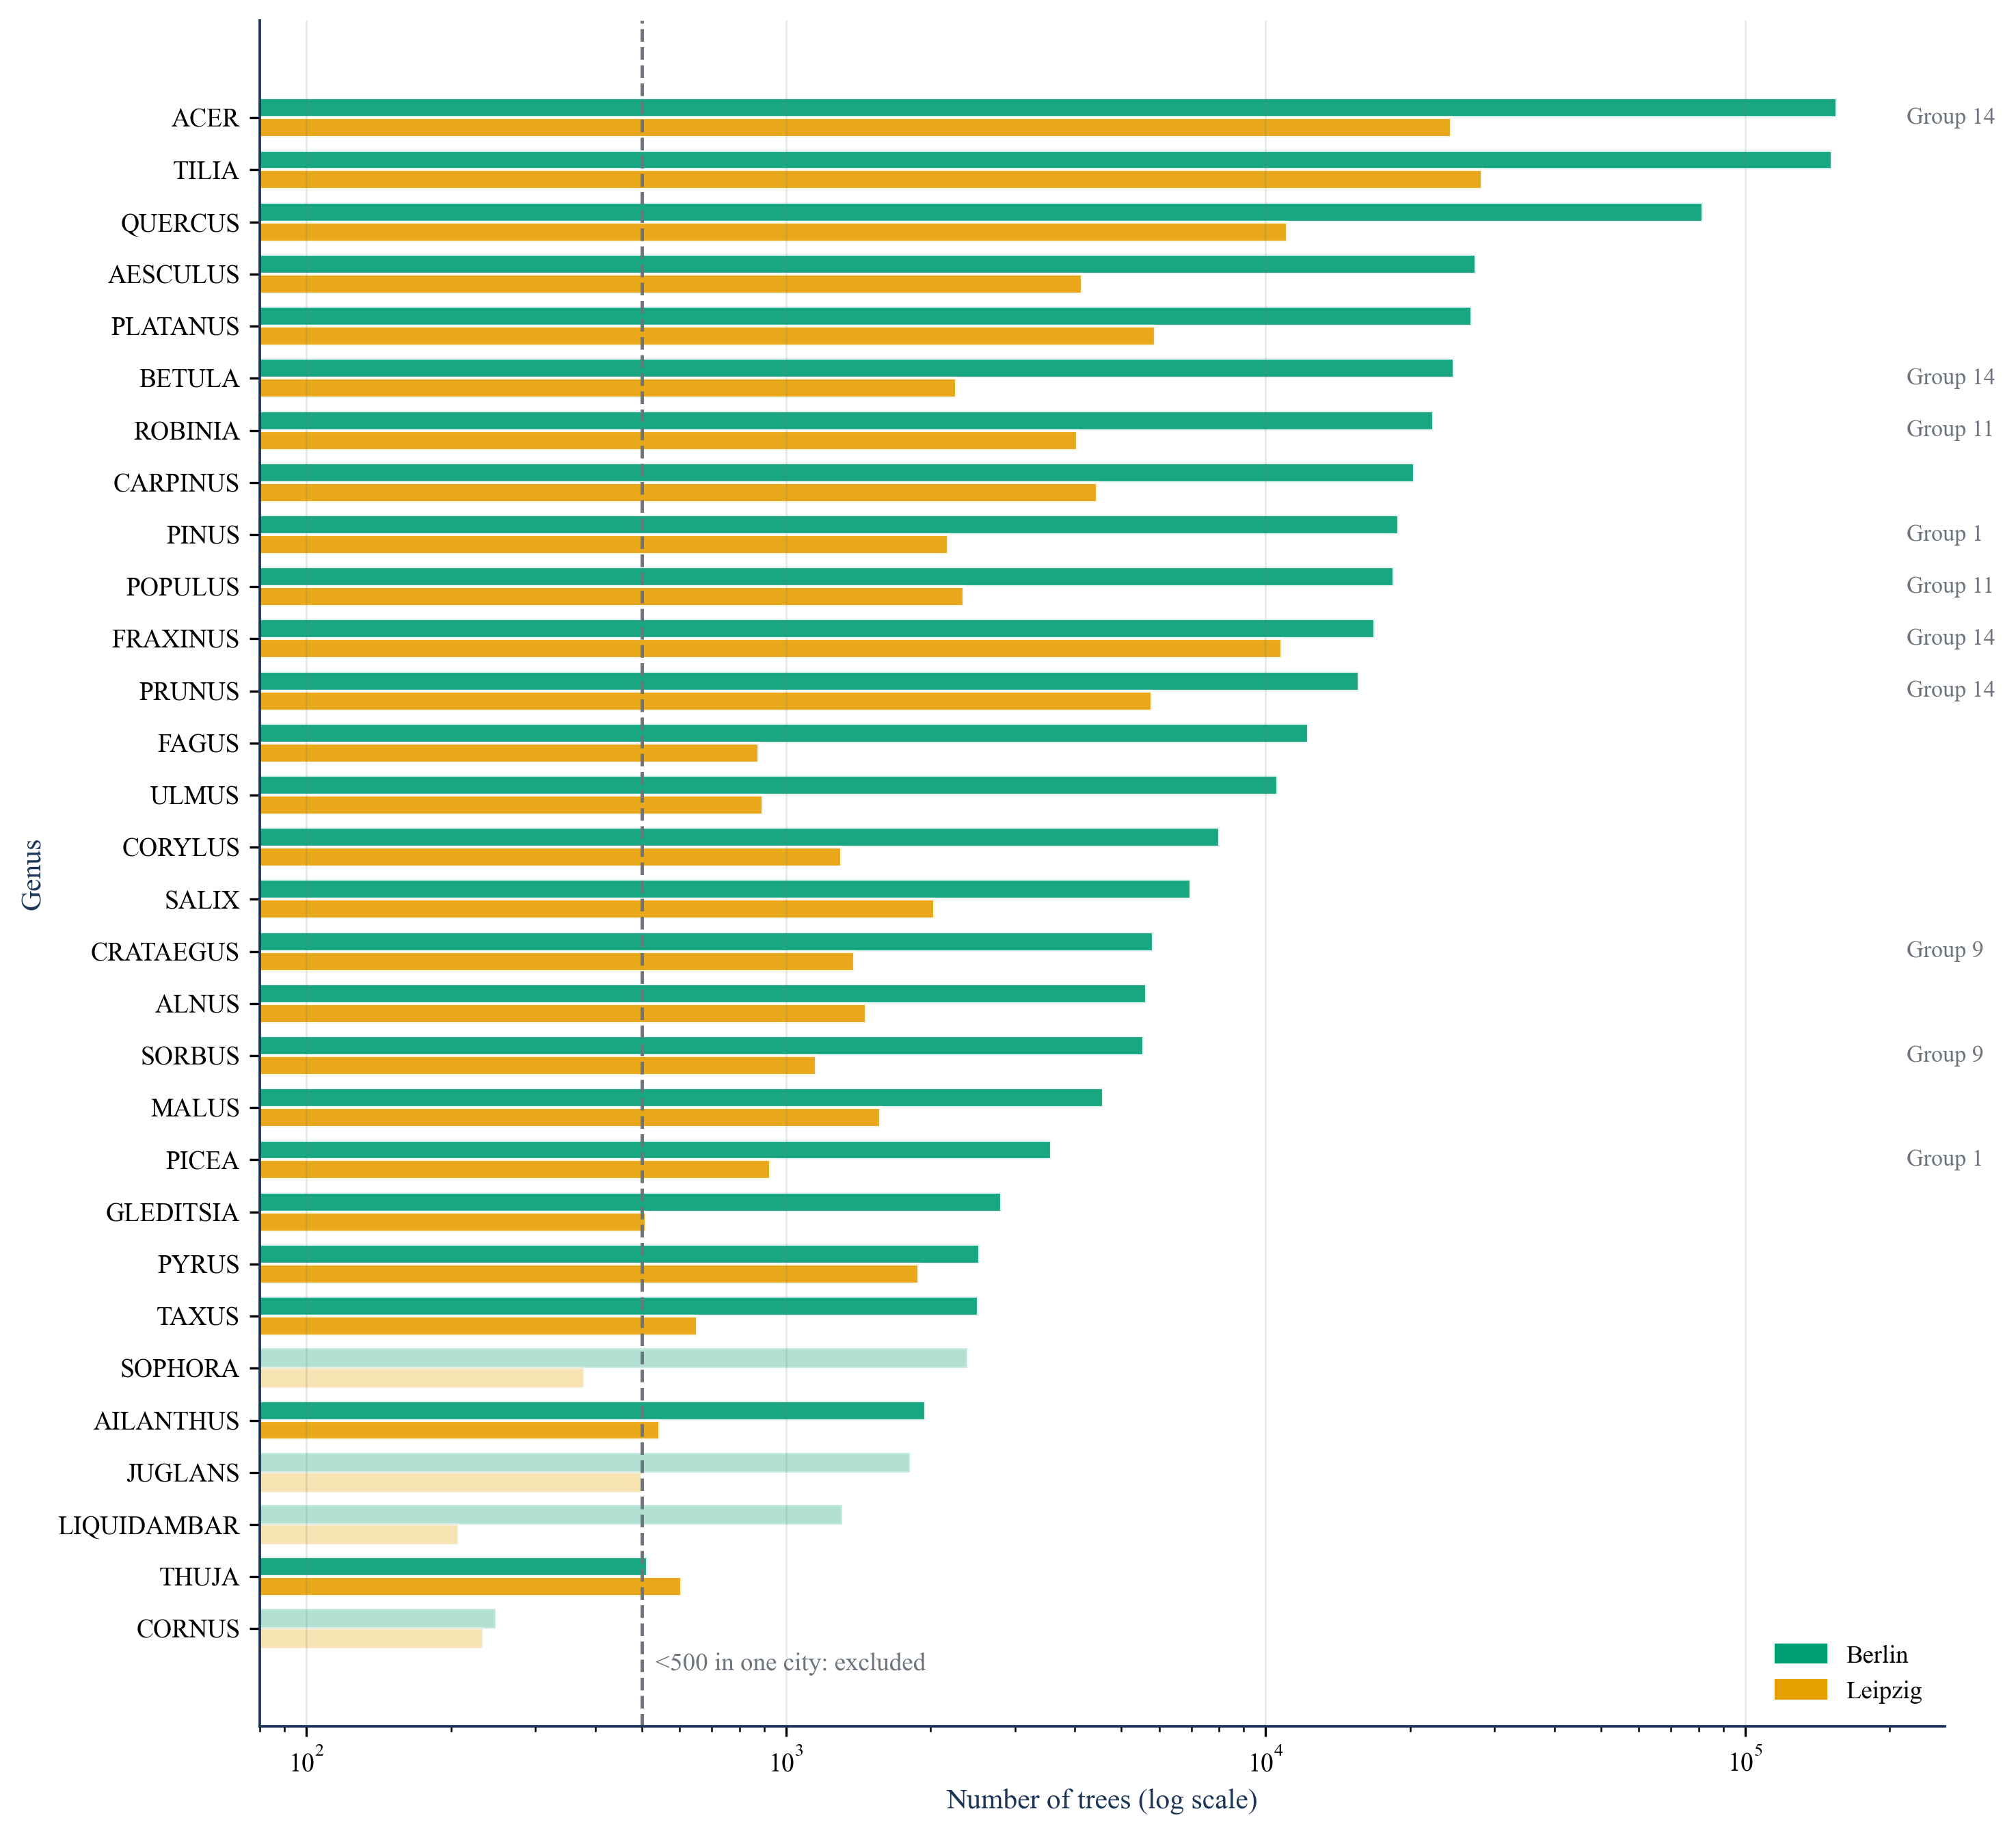
\includegraphics[width=0.80\linewidth,height=0.44\textheight,keepaspectratio]{figures/fig-genus-distribution.png}
  \caption{Genus distribution comparison between Berlin and Leipzig to visualise class imbalance and domain shift.}
  \label{fig:fig-genus-distribution}
\end{figure}

\subsection{Feature Engineering}\label{feature-engineering}

\subsubsection{Feature Construction and
Selection}\label{feature-construction-and-selection}

Prior to feature construction, CHM discriminative power and cross-city
transferability were assessed via Welch-ANOVA (η²) and Cohen's d
(\cref{fig:fig-chm-cohens-d}). The analysis confirmed that canopy height
provided genus-level discrimination while remaining sufficiently
consistent across cities for transfer.

Per-tree feature vectors were constructed by extracting spectral values
at each corrected tree location from the monthly composites. The initial
feature space comprised 10 spectral bands and 13 vegetation indices
across 12 months, totalling 276 features per tree. To reduce
dimensionality while preserving phenological information, months were
ranked by mean Jeffries-Matusita (JM) distance (Richards and Jia 2006)
across all genus pairs. Cross-city consistency of the monthly ranking
was verified (Spearman ρ = 0.951, p \textless{} 0.001), confirming that
discriminative months generalise across domains
(\cref{fig:fig-jm-monthly}). Eight months (April through November) were
retained, covering the full growing season from leaf flush through
senescence. Winter months contributed minimal separability and were
excluded, reducing the temporal feature space by 33\%.

\begin{figure}[H]
  \centering
  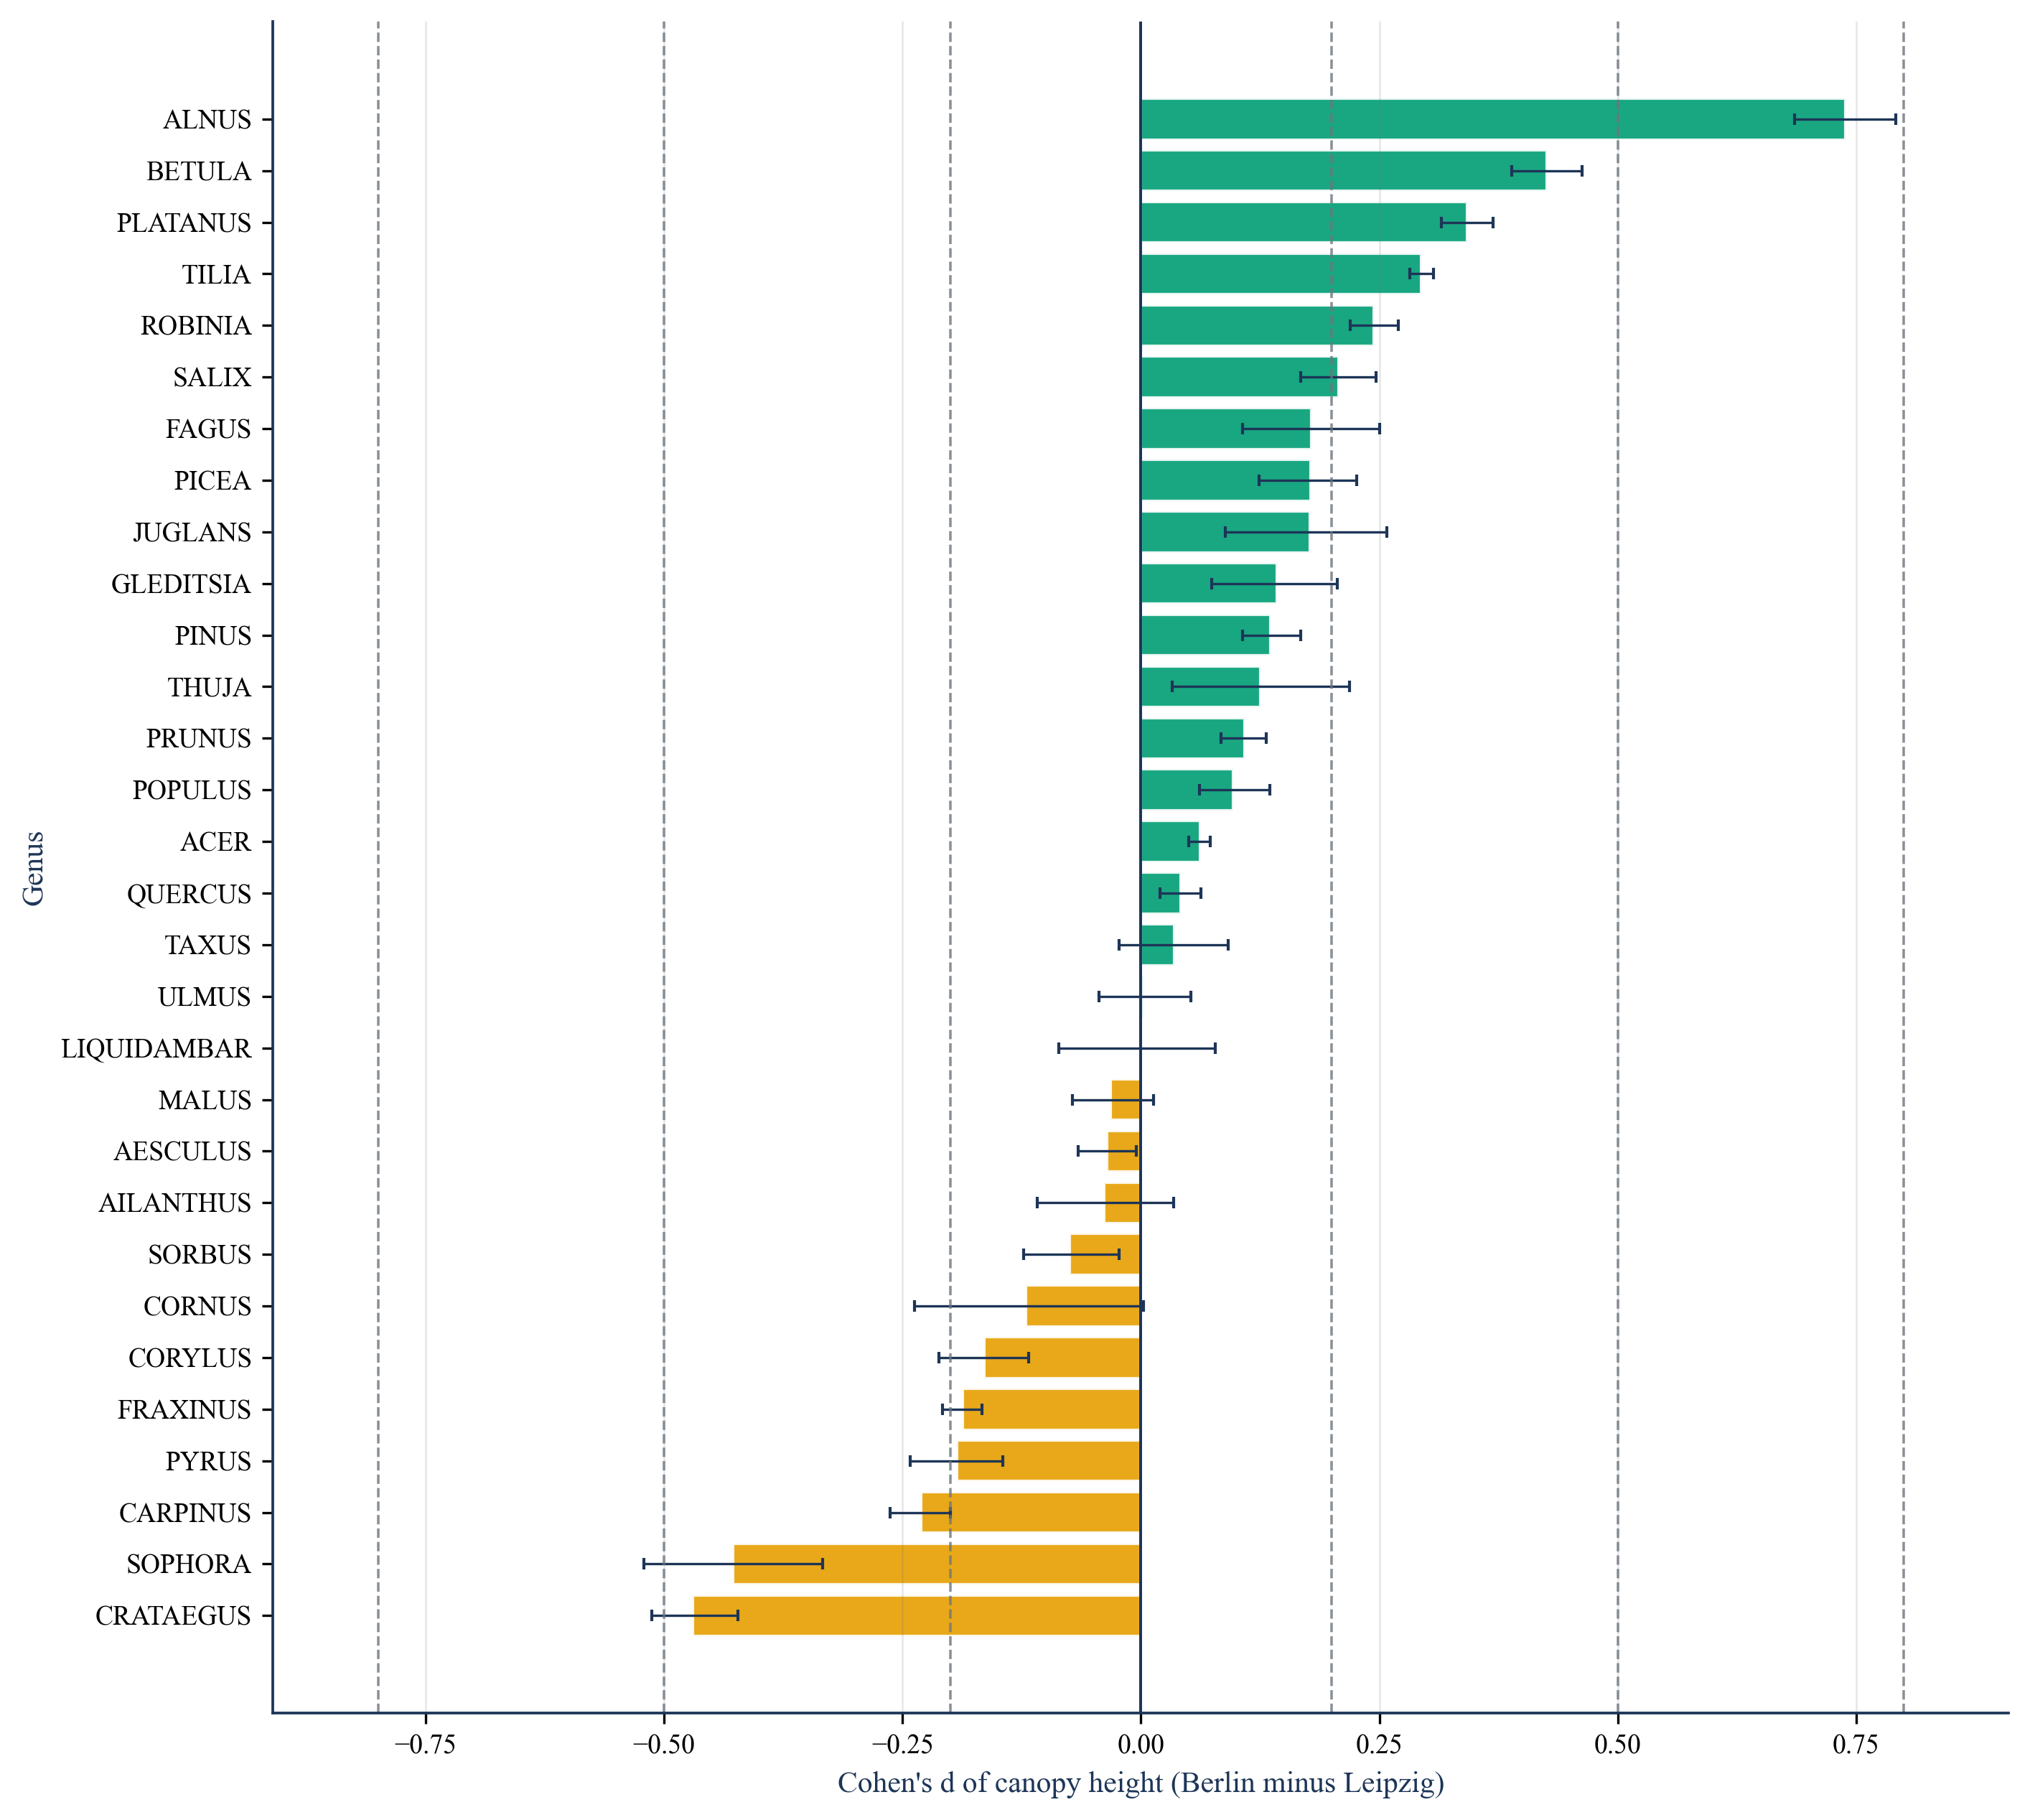
\includegraphics[width=0.80\linewidth,height=0.44\textheight,keepaspectratio]{figures/fig-chm-cohens-d.png}
  \caption{Cohen's d by genus for CHM transfer consistency assessment, showing the cross-city shift in canopy-height distributions between Berlin and Leipzig for each class.}
  \label{fig:fig-chm-cohens-d}
\end{figure}

\begin{figure}[H]
  \centering
  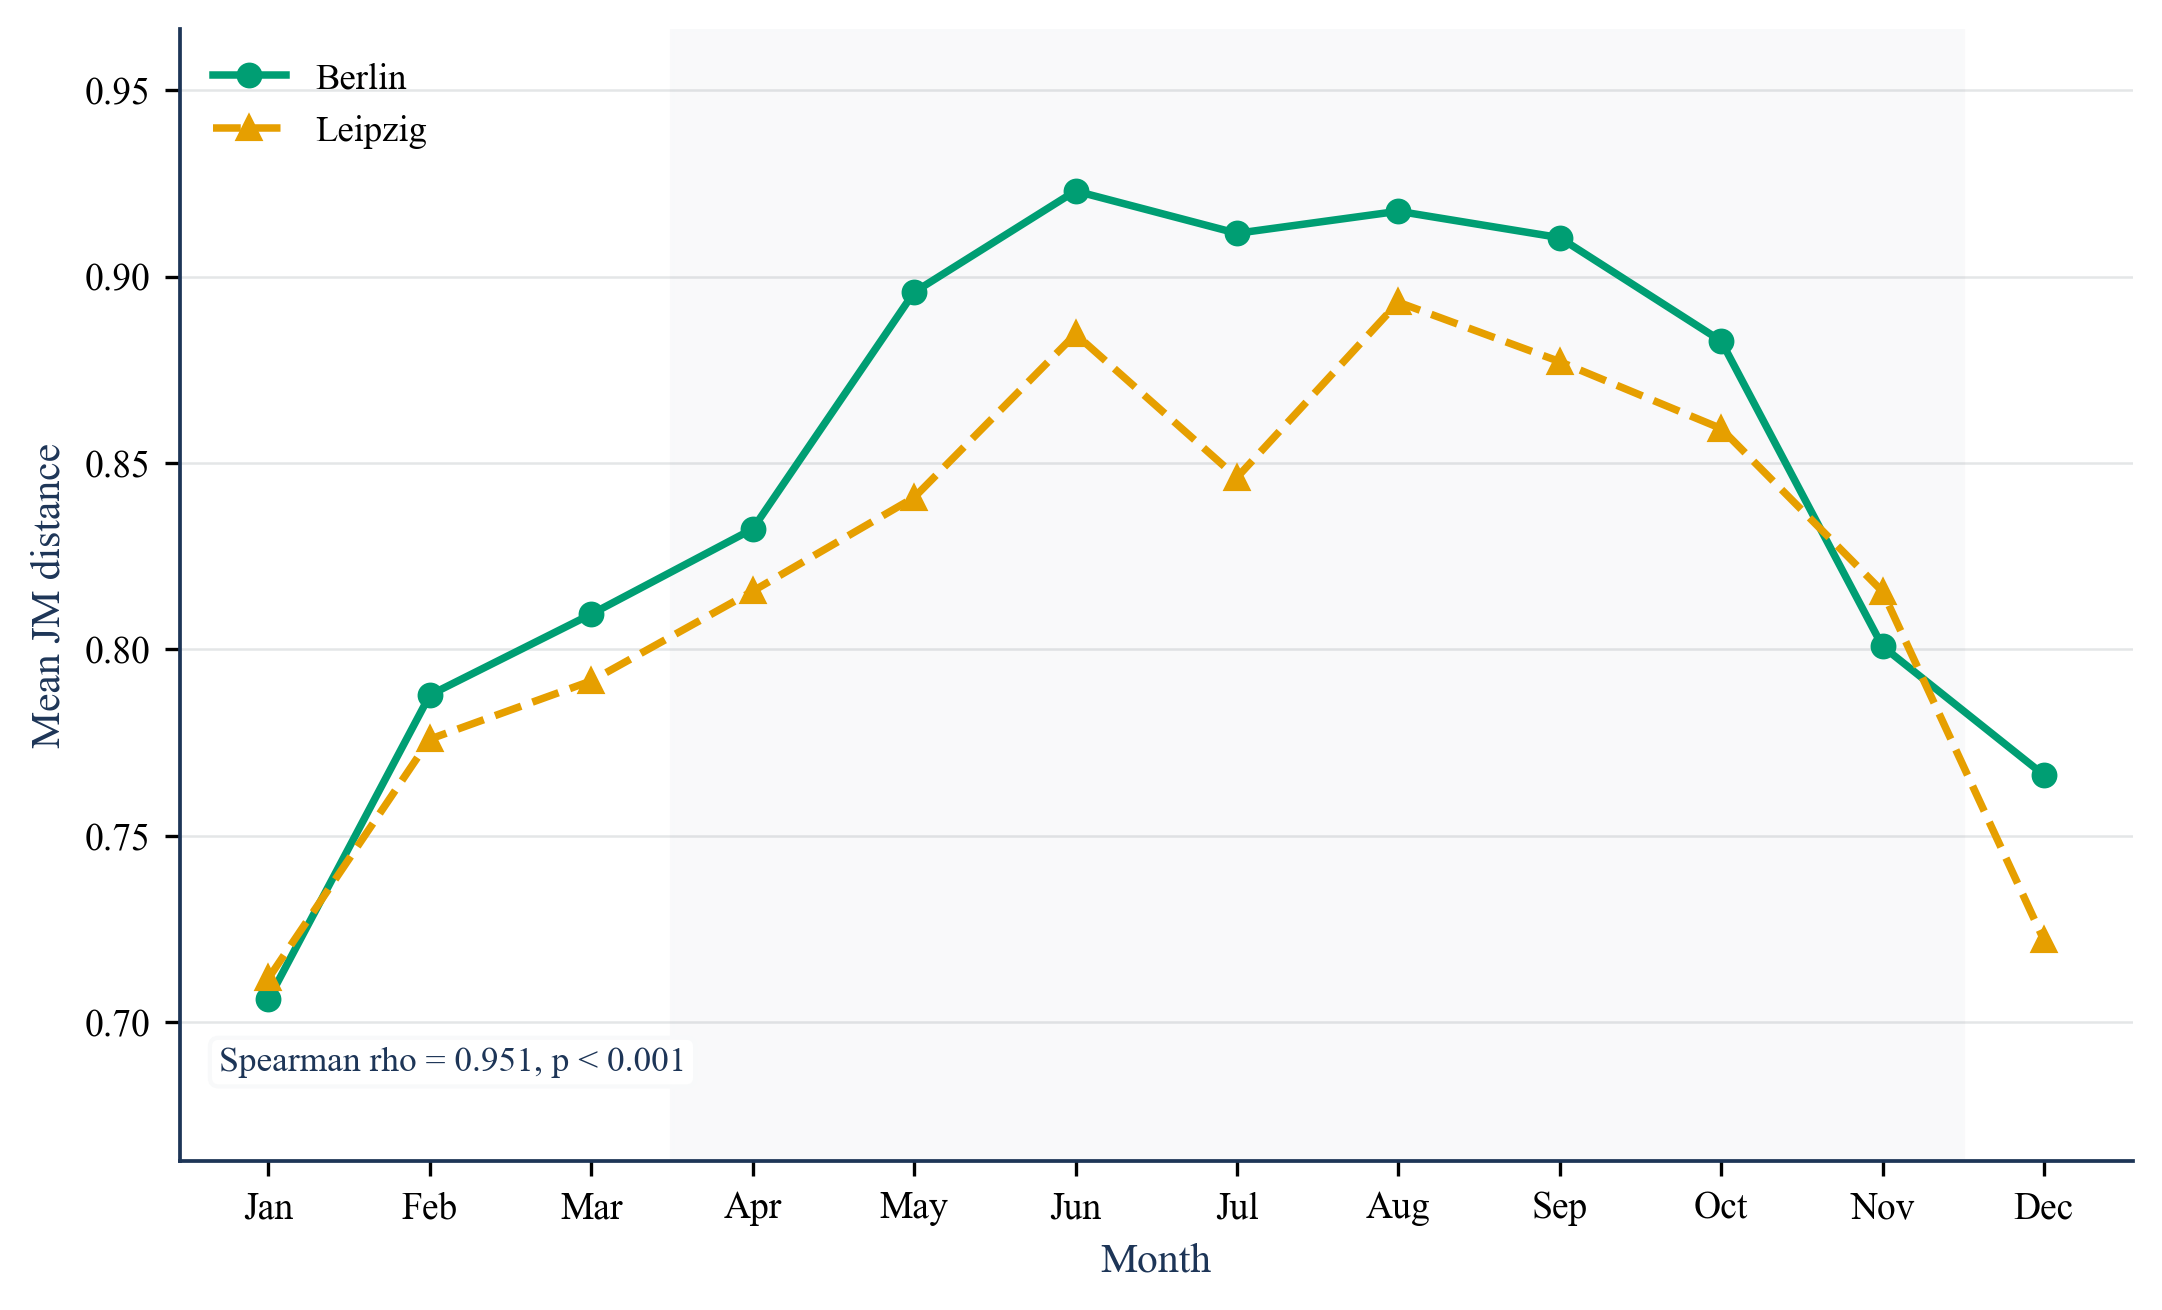
\includegraphics[width=0.82\linewidth,height=0.46\textheight,keepaspectratio]{figures/fig-jm-monthly.png}
  \caption{Monthly JM-distance ranking for Berlin and Leipzig, showing that the most discriminative acquisition periods are consistent across both cities.}
  \label{fig:fig-jm-monthly}
\end{figure}

Pairwise Pearson correlations were computed between all spectral
variables (bands and indices) across the temporal stack
(\cref{fig:fig-correlation}). For each pair of variables whose monthly
time series exceeded \textbar r\textbar{} \textgreater{} 0.95 in both
cities, the more redundant variable was dropped entirely, across all
retained months. Selection prioritised established indices and broader
spectral bands. Five variables were eliminated this way, removing 40
feature columns in total (5 variables × 8 months), and yielding a final
set of 147 features: 64 spectral band features (8 bands × 8 months), 80
vegetation index features (10 indices × 8 months: Chlorophyll Index
Red-Edge (CIre), Enhanced Vegetation Index (EVI), Inverted Red-Edge
Chlorophyll Index (IRECI), Moisture Stress Index (MSI), NDVI, NDVI
Red-Edge (NDVIre), Normalized Difference Water Index (NDWI), Normalized
Difference Red-Edge 1 (NDre1), Red-Edge Triangulated Vegetation Index
core (RTVIcore), and Visible Atmospherically Resistant Index (VARI)),
and 3 CHM features: the raw 1 m canopy height at the corrected crown
centre, and two engineered variants, a genus-level percentile rank and a
within-genus z-score, both derived from the Berlin training distribution
to normalise absolute height differences driven by site conditions and
tree age.

\begin{figure}[H]
  \centering
  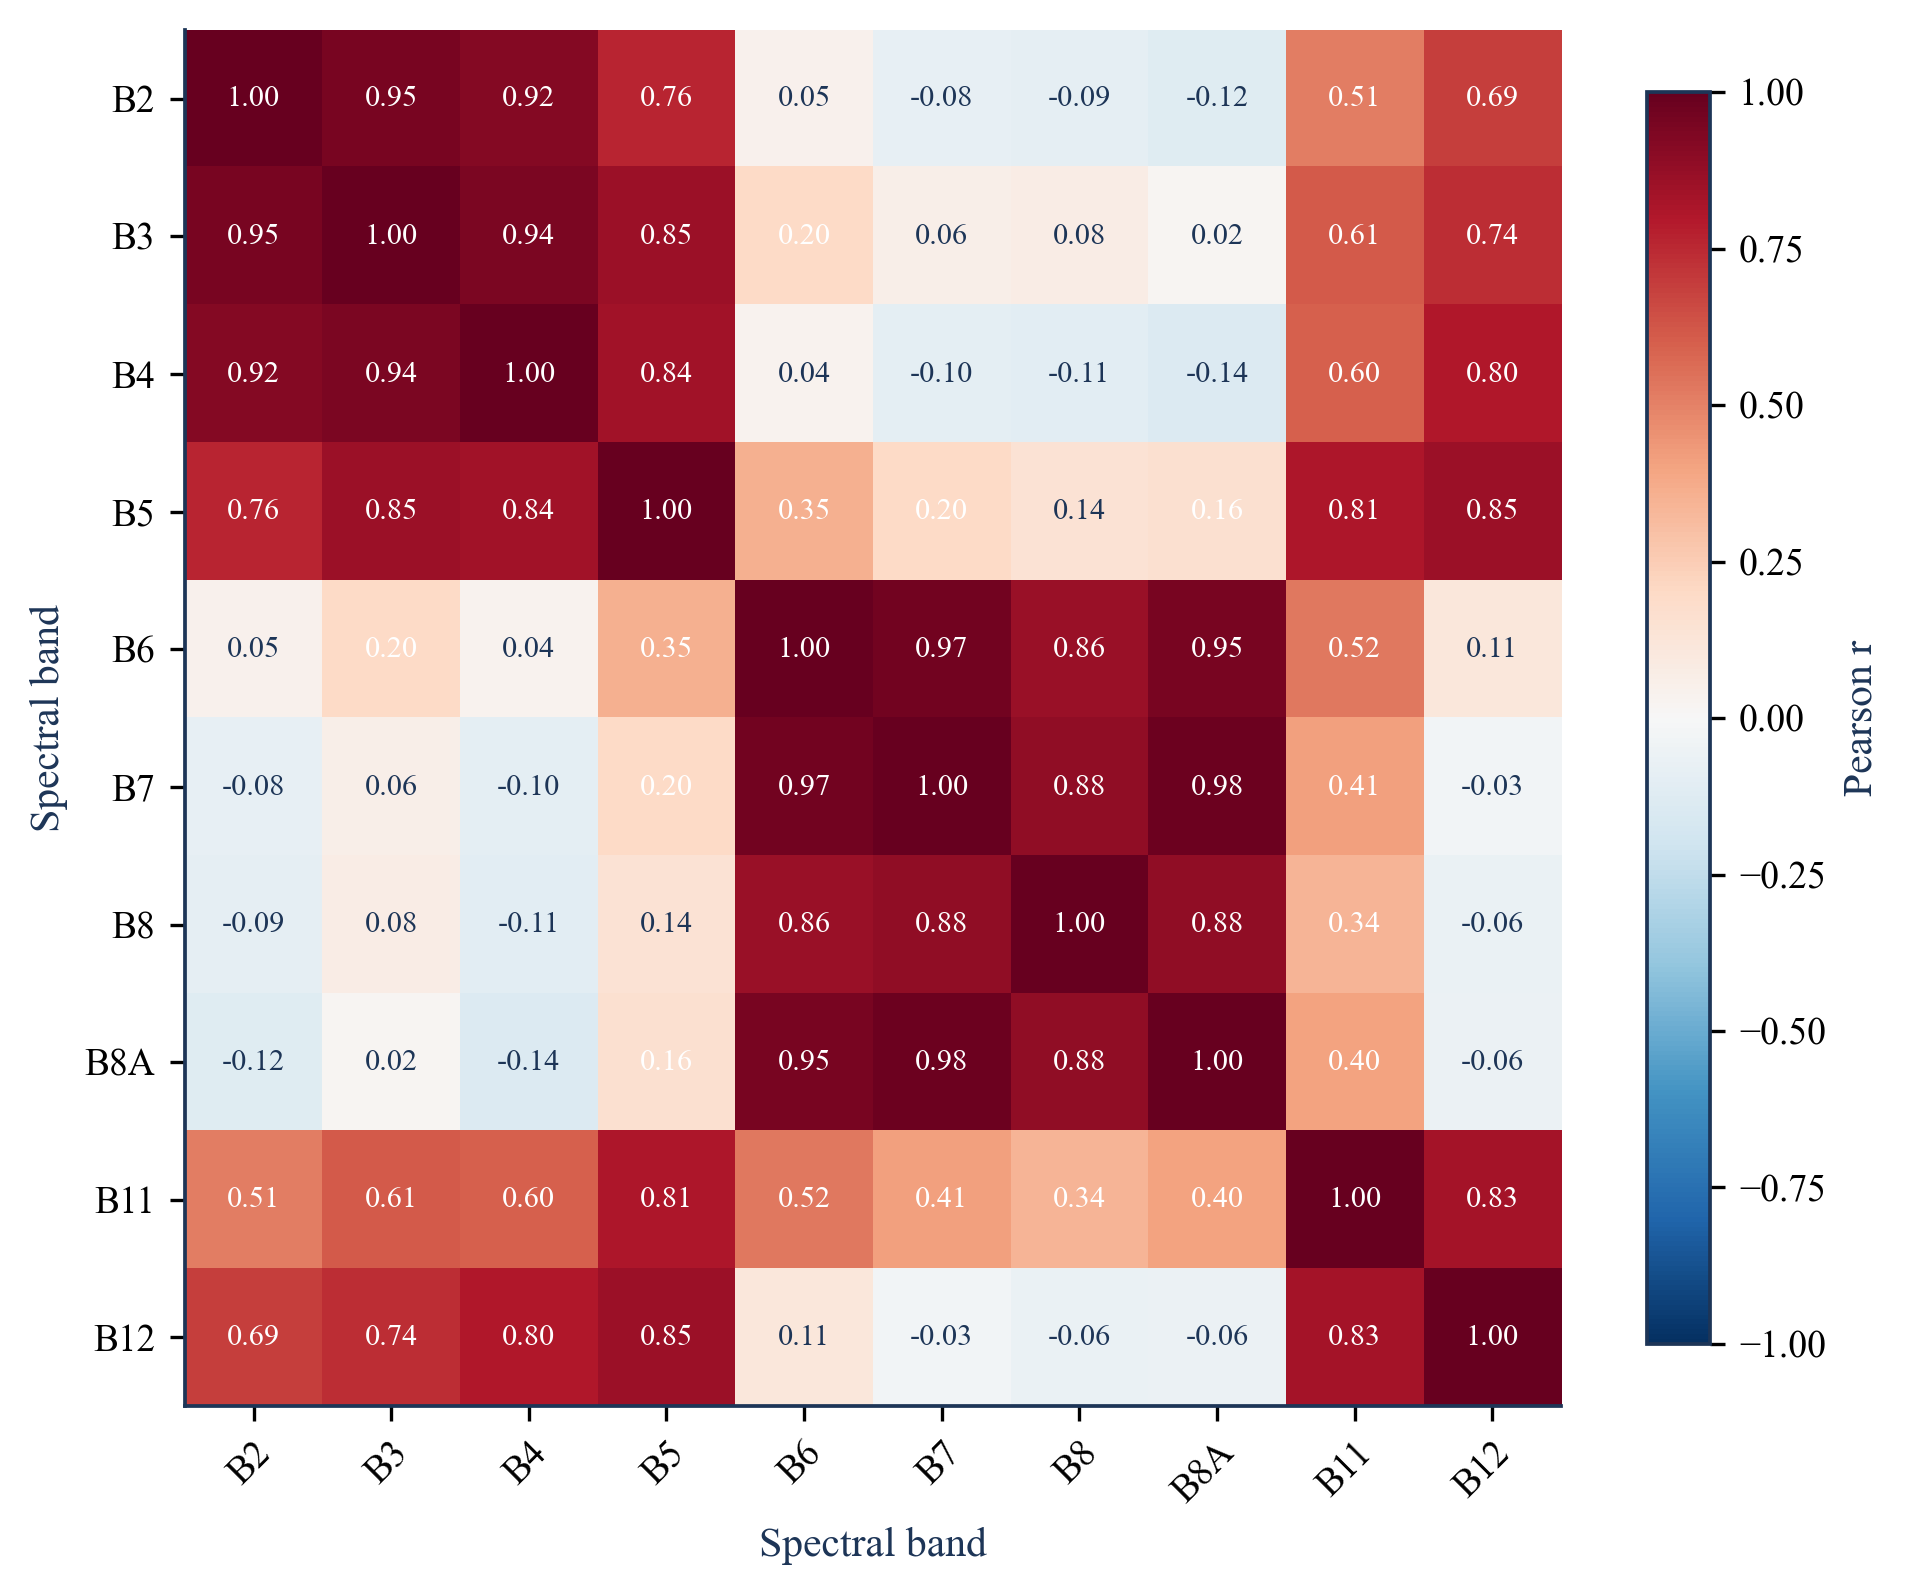
\includegraphics[width=0.86\linewidth,height=0.50\textheight,keepaspectratio]{figures/fig-correlation.png}
  \caption{Pearson correlation heatmap for spectral bands (indices excluded for clarity).}
  \label{fig:fig-correlation}
\end{figure}

To define the final class set, genera with fewer than 500 individuals
per city after quality filtering were excluded. Pairwise JM distances
were computed for all remaining genera on Berlin training data. Genera
falling below the 10th percentile of pairwise JM distance (P10 = 1.373)
were merged into groups. The resulting groups reflect two distinct
rationales (group numbers refer to the index position of genera in the
full genus list). Three groups are supported by both spectral similarity
and biological coherence: Group 1 (PICEA, PINUS: Pinaceae conifers with
stable year-round evergreen spectral signatures), Group 9 (CRATAEGUS,
SORBUS: Rosaceae with overlapping phenological cycles and crown
morphology), and Group 11 (POPULUS, ROBINIA: disturbance-tolerant
pioneer species with structurally similar canopies). One group is
defined by spectral indistinguishability alone: Group 14 (ACER, BETULA,
FRAXINUS, PRUNUS) comprises broad-leaved deciduous genera with no strong
shared biological affinity that could not be reliably separated at 10 m
Sentinel-2 resolution. It functions as a residual class for genera with
overlapping spectral-temporal profiles. This procedure resulted in 17
classes (13 single genera + 4 groups).

\subsubsection{Data Quality and Spatial
Design}\label{data-quality-and-spatial-design}

Trees planted after a CHM-derived threshold year (last cohort with
median canopy height ≥ 2.0 m) were excluded, as crowns below this height
are unlikely to produce a reliable spectral signal at 10 m Sentinel-2
resolution. An NDVI plausibility filter further removed trees whose
maximum NDVI across all retained months fell below 0.3, likely
indicating non-vegetated locations or dead trees. Trees with more than
two connected missing months (due to cloud masking) were excluded. Those
with up to two connected missing months were retained and gaps filled by
within-tree linear interpolation, with no cross-tree statistics used to
prevent data leakage. Together, these quality filters retained 91.7\% of
the original dataset (983,782 trees: 830,153 Berlin, 153,629 Leipzig).

Outlier detection combined three methods: univariate Z-scores
(\textbar z\textbar{} \textgreater{} 3 in ≥ 10 features), genus-specific
Mahalanobis distance {[}α = 0.001 with Ledoit-Wolf covariance shrinkage;
Ledoit and Wolf (2004){]}, and Interquartile Range (IQR) fences on CHM
values (k = 1.5). Trees were flagged by number of methods agreeing,
rather than removed, preserving the option for ablation in the
experimental phase. Of the total dataset, 95.9\% of trees were
classified as non-outliers.

At 10 m Sentinel-2 resolution, trees in close proximity to individuals
of different genera risk spectral contamination through pixel mixing.
Data retention rates were computed for minimum separation thresholds of
5, 10, 15, and 20 m to the nearest different-genus neighbour, yielding
retention of 79.4\%, 51.1\%, 34.7\%, and 26.2\%, respectively. The 5 m
threshold was selected as the smallest distance exceeding approximately
twice the Sentinel-2 pixel size (10 m), providing a minimum spectral
buffer while preserving the largest feasible training set. A
classification ablation confirmed a +2.7 pp weighted F1 improvement over
the unfiltered baseline, retaining 659,266 Berlin and 122,756 Leipzig
trees (782,022 combined, 79.5\% of the quality-filtered dataset). Both
the filtered and unfiltered datasets were carried through the
experimental pipeline to assess the effect of spectral purity on
classification performance.

Spatial autocorrelation was quantified using Moran's I (Moran 1950) at
distance lags from 100 m to 1200 m for five representative features per
city (\cref{fig:fig-morans-i}). Autocorrelation decayed consistently in
both cities, with residual I values of 0.185 (Berlin) and 0.154
(Leipzig) at 1200 m. A block size of 1200 m was adopted for spatial CV
to minimise information leakage between folds.

\begin{figure}[!htbp]
  \centering
  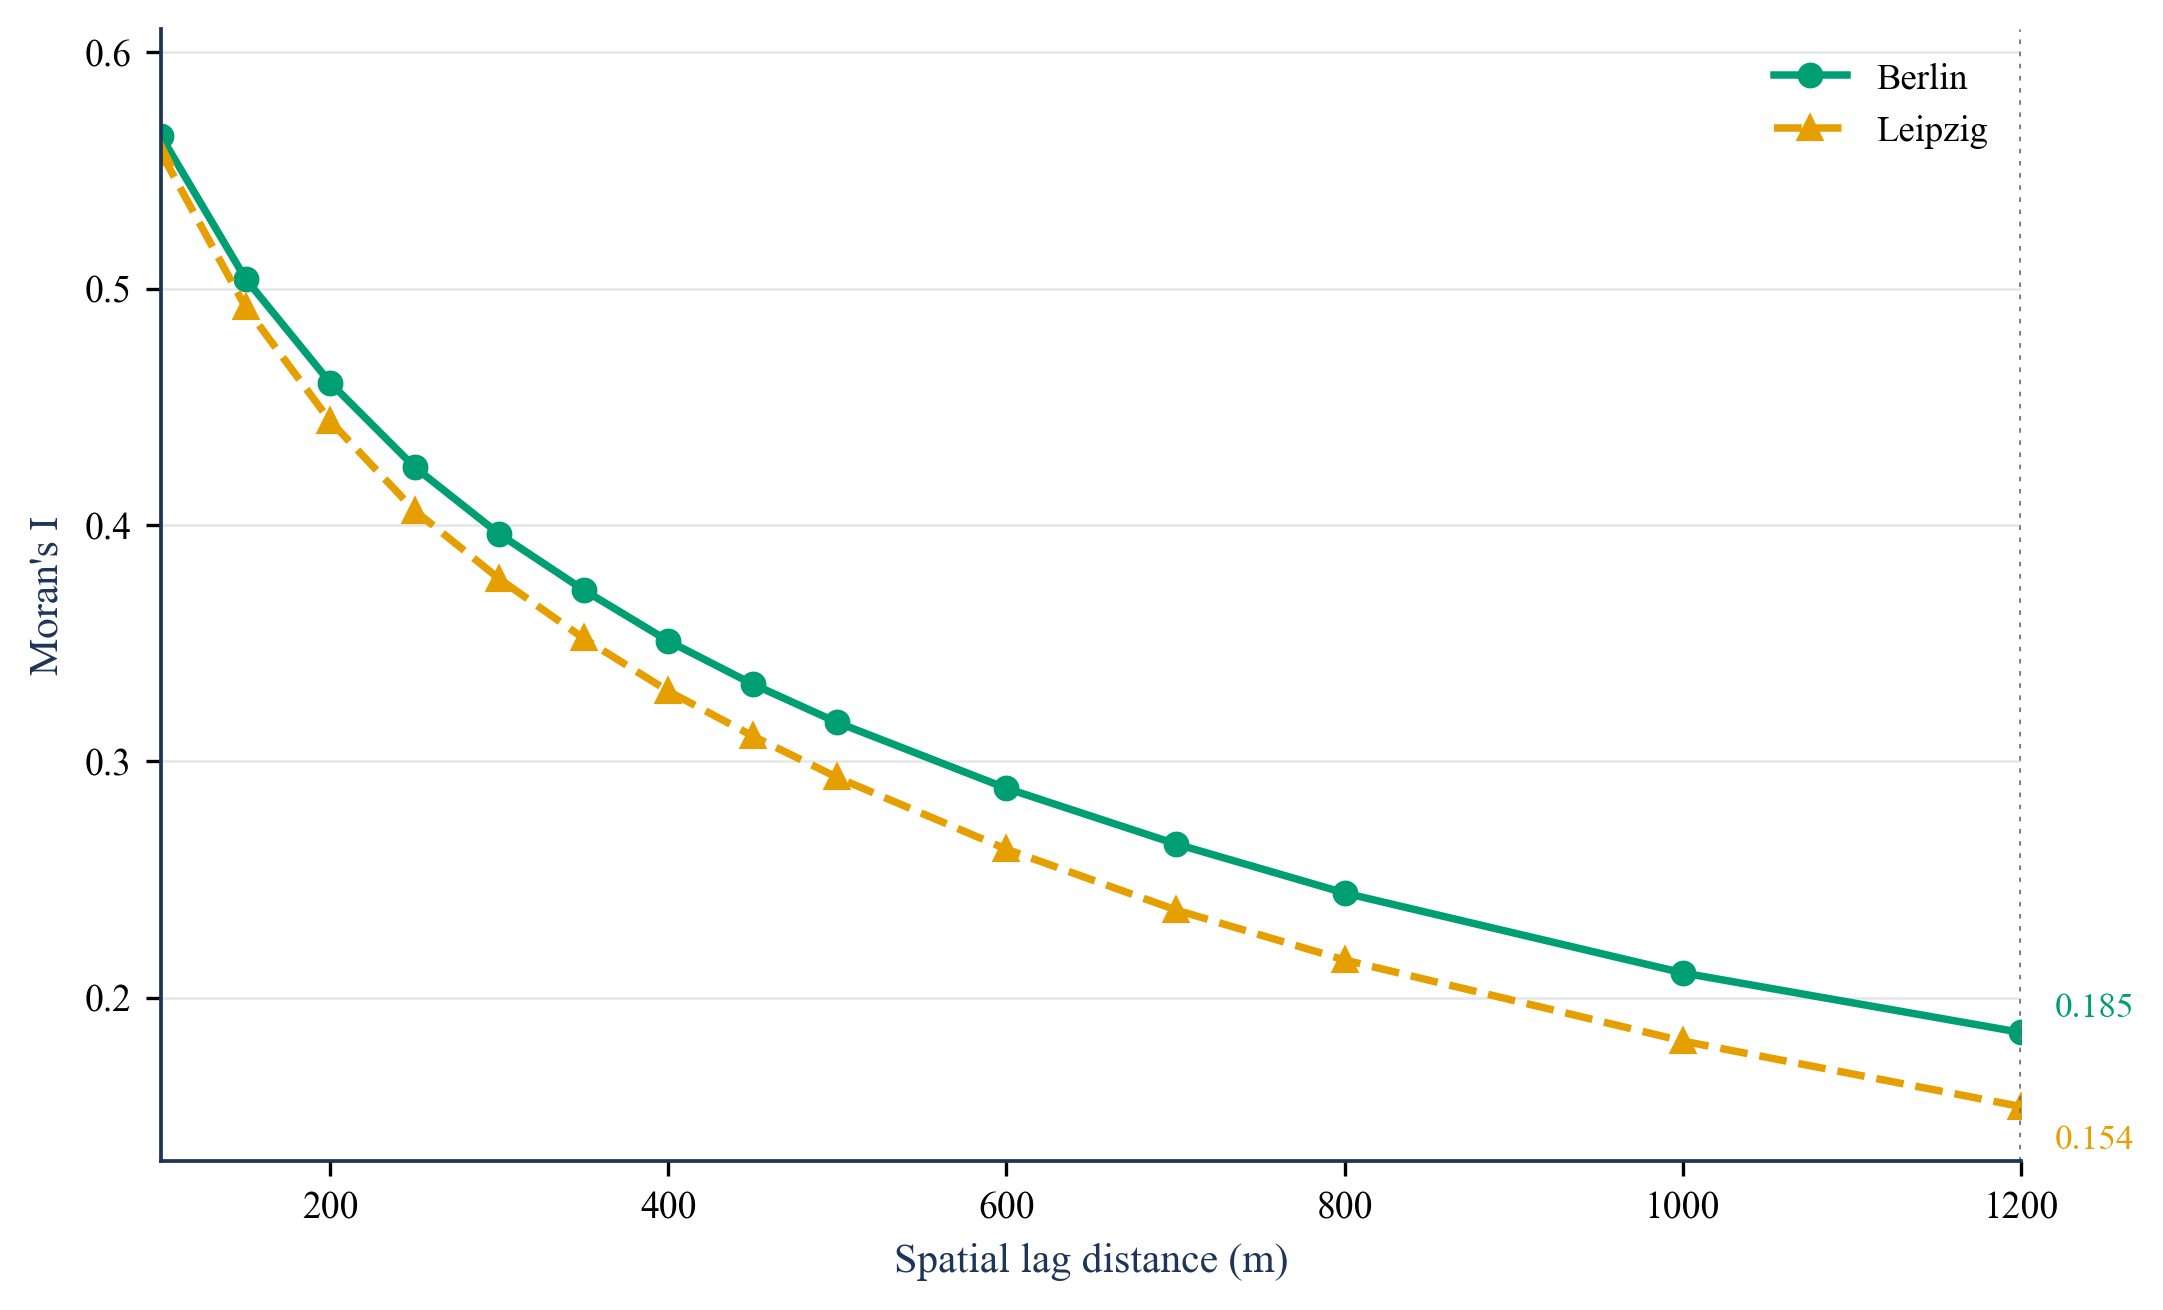
\includegraphics[width=0.84\linewidth,height=0.50\textheight,keepaspectratio]{figures/fig-morans-i.png}
  \caption{Moran's I decay curves by distance for Berlin and Leipzig.}
  \label{fig:fig-morans-i}
\end{figure}

Spatial blocks were assigned to train/validation/test splits for Berlin
(target ratio 70/15/15) and finetune/test splits for Leipzig (80/20).
Split quality was controlled via Kullback-Leibler (KL) divergence on
genus distributions (all splits \textless{} 0.07). The threshold of 0.07
was empirically relaxed from the common standard of 0.05 to accommodate
constraints imposed by spatial blocking and proximity filtering, which
limit the combinatorial freedom for balanced genus proportions across
splits. After all processing steps, two parallel datasets were carried
forward: the unfiltered baseline (983,782 trees: 830,153 Berlin, 153,629
Leipzig) and the proximity-filtered training dataset (782,022 trees:
659,266 Berlin, 122,756 Leipzig), both with 147 features each.

\subsection{Experimental Setup}\label{experimental-setup}

\subsubsection{Setup Fixation}\label{setup-fixation}

All setup decisions, including CHM inclusion, proximity filtering,
outlier removal, and feature count, were fixed prior to the algorithm
comparison. All classifiers therefore received identical data, isolating
algorithmic effects on performance. Setup decisions were determined
through sequential ablation studies using RF as a computationally
efficient, deterministic baseline that provides stable feature
importance rankings and exhibits low overfitting, making it suitable for
isolating data-level effects without confounding them with model-level
variance. Ablations followed the order CHM → proximity → outlier →
features, with each decision building on the preceding one. All
ablations were evaluated under 3-fold spatial block CV on Berlin data
only, with no Leipzig data entering setup decisions.

Sequential ablation on Berlin training data produced four configuration
decisions. CHM was excluded: all CHM variants increased the
train-validation gap by 9--14 pp with weighted F1 gains below 0.8 pp,
indicating city-specific overfitting despite the genus-level
discriminative power confirmed in the CHM assessment (Section 4.2.1).
Outlier removal produced no measurable weighted F1 improvement across
all severity levels and was therefore not applied. Feature reduction
identified the Top-50 importance-ranked features as the optimal subset,
matching full-feature performance within 1 pp while reducing the
spectral-temporal feature space from 144 to 50.

\subsubsection{Models and Training}\label{models-and-training}

Four classifiers were evaluated across two algorithmic paradigms: RF and
XGBoost (Chen and Guestrin 2016) for ML, and the 1D-CNN and TabNet for
DL (Section 2.3). Within each paradigm, a coarse grid search (24--48
configurations per algorithm, 3-fold spatial block CV) identified the
stronger candidate based on validation weighted F1 and train-validation
gap: XGBoost for the ML paradigm and the 1D-CNN for the DL paradigm. The
two champions were carried forward for fine-grained hyperparameter
optimisation and all subsequent experiments.

Different feature representations were used for each paradigm,
reflecting the distinct inductive biases of each model class. ML models
(RF, XGBoost) received 50 importance-ranked features from the
144-feature spectral-temporal pool, as tree-based models benefit from
dimensionality reduction that removes redundant splits. DL models
(1D-CNN, TabNet) received the full 144 spectral-temporal features (18
variables × 8 months, excluding CHM) to preserve the temporal continuity
required for convolutional filters. Champion selection within each
paradigm was based on validation weighted F1 together with the
train-validation gap to avoid carrying forward overfitted models; under
this criterion, XGBoost and the 1D-CNN were selected as the ML and DL
champions, respectively. This design choice means that performance
differences between paradigms reflect the combined effect of algorithm
and feature representation, not algorithm alone (Section 6.6). All four
classifiers incorporated class balancing to compensate for
genus-frequency imbalance: RF and XGBoost through inverse-frequency
sample weighting, the 1D-CNN and TabNet through class-weighted loss
functions.

Fine-grained hyperparameter optimisation of the two champions was
performed via Optuna (Akiba et al. 2019); final configurations are
listed in the appendix (\cref{tbl:tbl-hyperparams-xgboost},
\cref{tbl:tbl-hyperparams-cnn}). Final models were retrained on combined
train and validation splits and evaluated once on the held-out Berlin
test set. Three naive baselines established lower performance bounds: a
majority-class classifier, a stratified random classifier, and a
spatial-only RF trained on Universal Transverse Mercator (UTM)
coordinates alone to test whether spatial autocorrelation provides
discriminative signal.

\subsubsection{Experimental Design}\label{experimental-design}

Three sequential experiments were conducted.

\emph{Experiment 1 (Berlin Optimisation)} established upper-bound
performance on the source domain. Both champions were trained,
optimised, and evaluated on the Berlin test set. Post-training error
analysis included per-genus precision, recall, and weighted F1,
confusion patterns, and feature importance ranking.

\emph{Experiment 2 (Zero-Shot Transfer)} applied the Berlin-trained
champions directly to the Leipzig test set without any adaptation. The
Berlin-fitted feature scaler was reused (transform only, no refit) to
ensure genuine zero-shot evaluation. Transfer performance was measured
as absolute and relative weighted F1 drop, with per-genus robustness
analysis.

\emph{Experiment 3 (Fine-Tuning)} fine-tuned both champions on
stratified Leipzig subsets at four data fractions (10\%, 25\%, 50\%,
100\%). For XGBoost, warm-start continuation was used (additional trees
appended to the Berlin ensemble). The 1D-CNN was fine-tuned at 10\% of
the original learning rate to prevent catastrophic forgetting. Class
weights were recomputed on the Leipzig distribution. A from-scratch
XGBoost baseline, trained exclusively on Leipzig with a Leipzig-fitted
scaler, served as the reference for transfer advantage. A from-scratch
1D-CNN baseline was not trained due to resource constraints.

Four hypotheses were pre-registered before execution to prevent post-hoc
bias: H1 (Genus Heterogeneity) posited that transfer loss varies
significantly across genera; H2 (Conifer Robustness) predicted that
evergreen genera exhibit smaller transfer losses due to more stable
year-round spectral signatures (Persson et al. 2018); although only one
conifer group was present in the final class set, the hypothesis was
retained as a structured template for future multi-city studies with
richer conifer representation; H3 (Spectral Separability) expected that
genera with higher JM distance in the source domain retain higher
classification accuracy after transfer; and H4 (Fine-Tuning Efficiency)
hypothesised that genera with larger zero-shot transfer gaps require
disproportionately more fine-tuning data for performance recovery.

\subsection{Evaluation Framework}\label{evaluation-framework}

The primary evaluation metric was weighted F1, which accounts for class
imbalance by weighting per-genus F1 proportionally to class frequency.
Secondary metrics included macro F1 (unweighted average), OA, and
per-genus precision, recall, and F1. Confidence intervals were computed
using percentile bootstrap with 1,000 resamples at the 95\% confidence
level. All ablations and algorithm comparisons were evaluated under
3-fold spatial block CV with 1200 m blocks.

Final evaluation was performed on held-out test sets: the Berlin test
set (15\% of Berlin data, block-assigned) and the Leipzig test set (20\%
of Leipzig data, block-assigned), both spatially disjoint from all
training and validation data at block level. An asymmetric proximity
policy was applied: train, validation, and fine-tuning splits used
proximity-filtered data to provide a spectrally pure training signal,
while test splits in both cities remained unfiltered, reflecting
real-world deployment conditions rather than laboratory settings.

Transfer performance was quantified through absolute drop (F1\_Berlin −
F1\_Leipzig), relative drop ((F1\_Berlin − F1\_Leipzig) / F1\_Berlin ×
100), and per-genus robustness categories (\textless5\% robust, 5--15\%
moderate, \textgreater15\% poor). Statistical tests comprised
Kruskal-Wallis H (H1), Mann-Whitney U (H2), and Spearman rank
correlation (H3, H4), all at α = 0.05, with McNemar's test for
classifier pair comparisons (zero-shot vs.~fine-tuned, fine-tuned
vs.~from-scratch). A power-law function (Performance = a × N\^{}b) was
fitted to the sample-efficiency curves as a descriptive characterisation
of recovery trajectory shape. With only four data fractions, the
two-parameter fit summarises the observed trend and enable comparison
with published saturation patterns, not for extrapolation beyond
observed data points.

\section{Results}\label{results}

\begin{table}[!htbp]
  \centering
  \small
  \caption{Summary of final weighted F1 results across source-domain, zero-shot, fine-tuned, and from-scratch settings.}
  \label{tbl:tbl-main-results}
  \begin{adjustbox}{max width=\linewidth}
  \begin{tabularx}{\linewidth}{>{\raggedright\arraybackslash}X>{\raggedright\arraybackslash}X>{\raggedright\arraybackslash}X>{\raggedright\arraybackslash}X>{\raggedright\arraybackslash}X}
  \toprule
  Model / Setting & Berlin Test weighted F1 & Leipzig Zero-Shot weighted F1 & Leipzig Fine-Tuned (100\%) weighted F1 & Leipzig From-Scratch weighted F1 \\
  \midrule
  XGBoost & 0.751 & 0.377 & 0.771 & 0.786 \\
  1D-CNN & 0.607 & 0.380 & 0.458 & -- \\
  \bottomrule
  \end{tabularx}
  \end{adjustbox}
\end{table}

\subsection{Berlin Optimisation}\label{berlin-optimisation}

The final weighted F1 results across source-domain, zero-shot,
fine-tuned, and from-scratch settings are summarised in
\cref{tbl:tbl-main-results}. The algorithm comparison established
performance baselines and identified champion models
(\cref{fig:fig-algorithm-comparison}). Naive baselines confirmed the
difficulty of the 17-class task: majority-class prediction achieved
weighted F1 = 0.182, and stratified random prediction reached weighted
F1 = 0.188. Among the four evaluated classifiers, RF attained validation
weighted F1 = 0.475 but exhibited severe overfitting (train-validation
gap = 0.398). XGBoost reached validation weighted F1 = 0.510 with
considerably less overfitting (gap = 0.138). TabNet reached validation
weighted F1 = 0.546 but exhibited substantially higher overfitting (gap
= 0.205), ruling it out as DL champion despite its competitive score.
The 1D-CNN achieved the highest validation weighted F1 = 0.567 with
minimal overfitting (gap = 0.047). XGBoost and the 1D-CNN were carried
forward as champions representing the ML and DL paradigms, respectively.

\begin{figure}[!htbp]
  \centering
  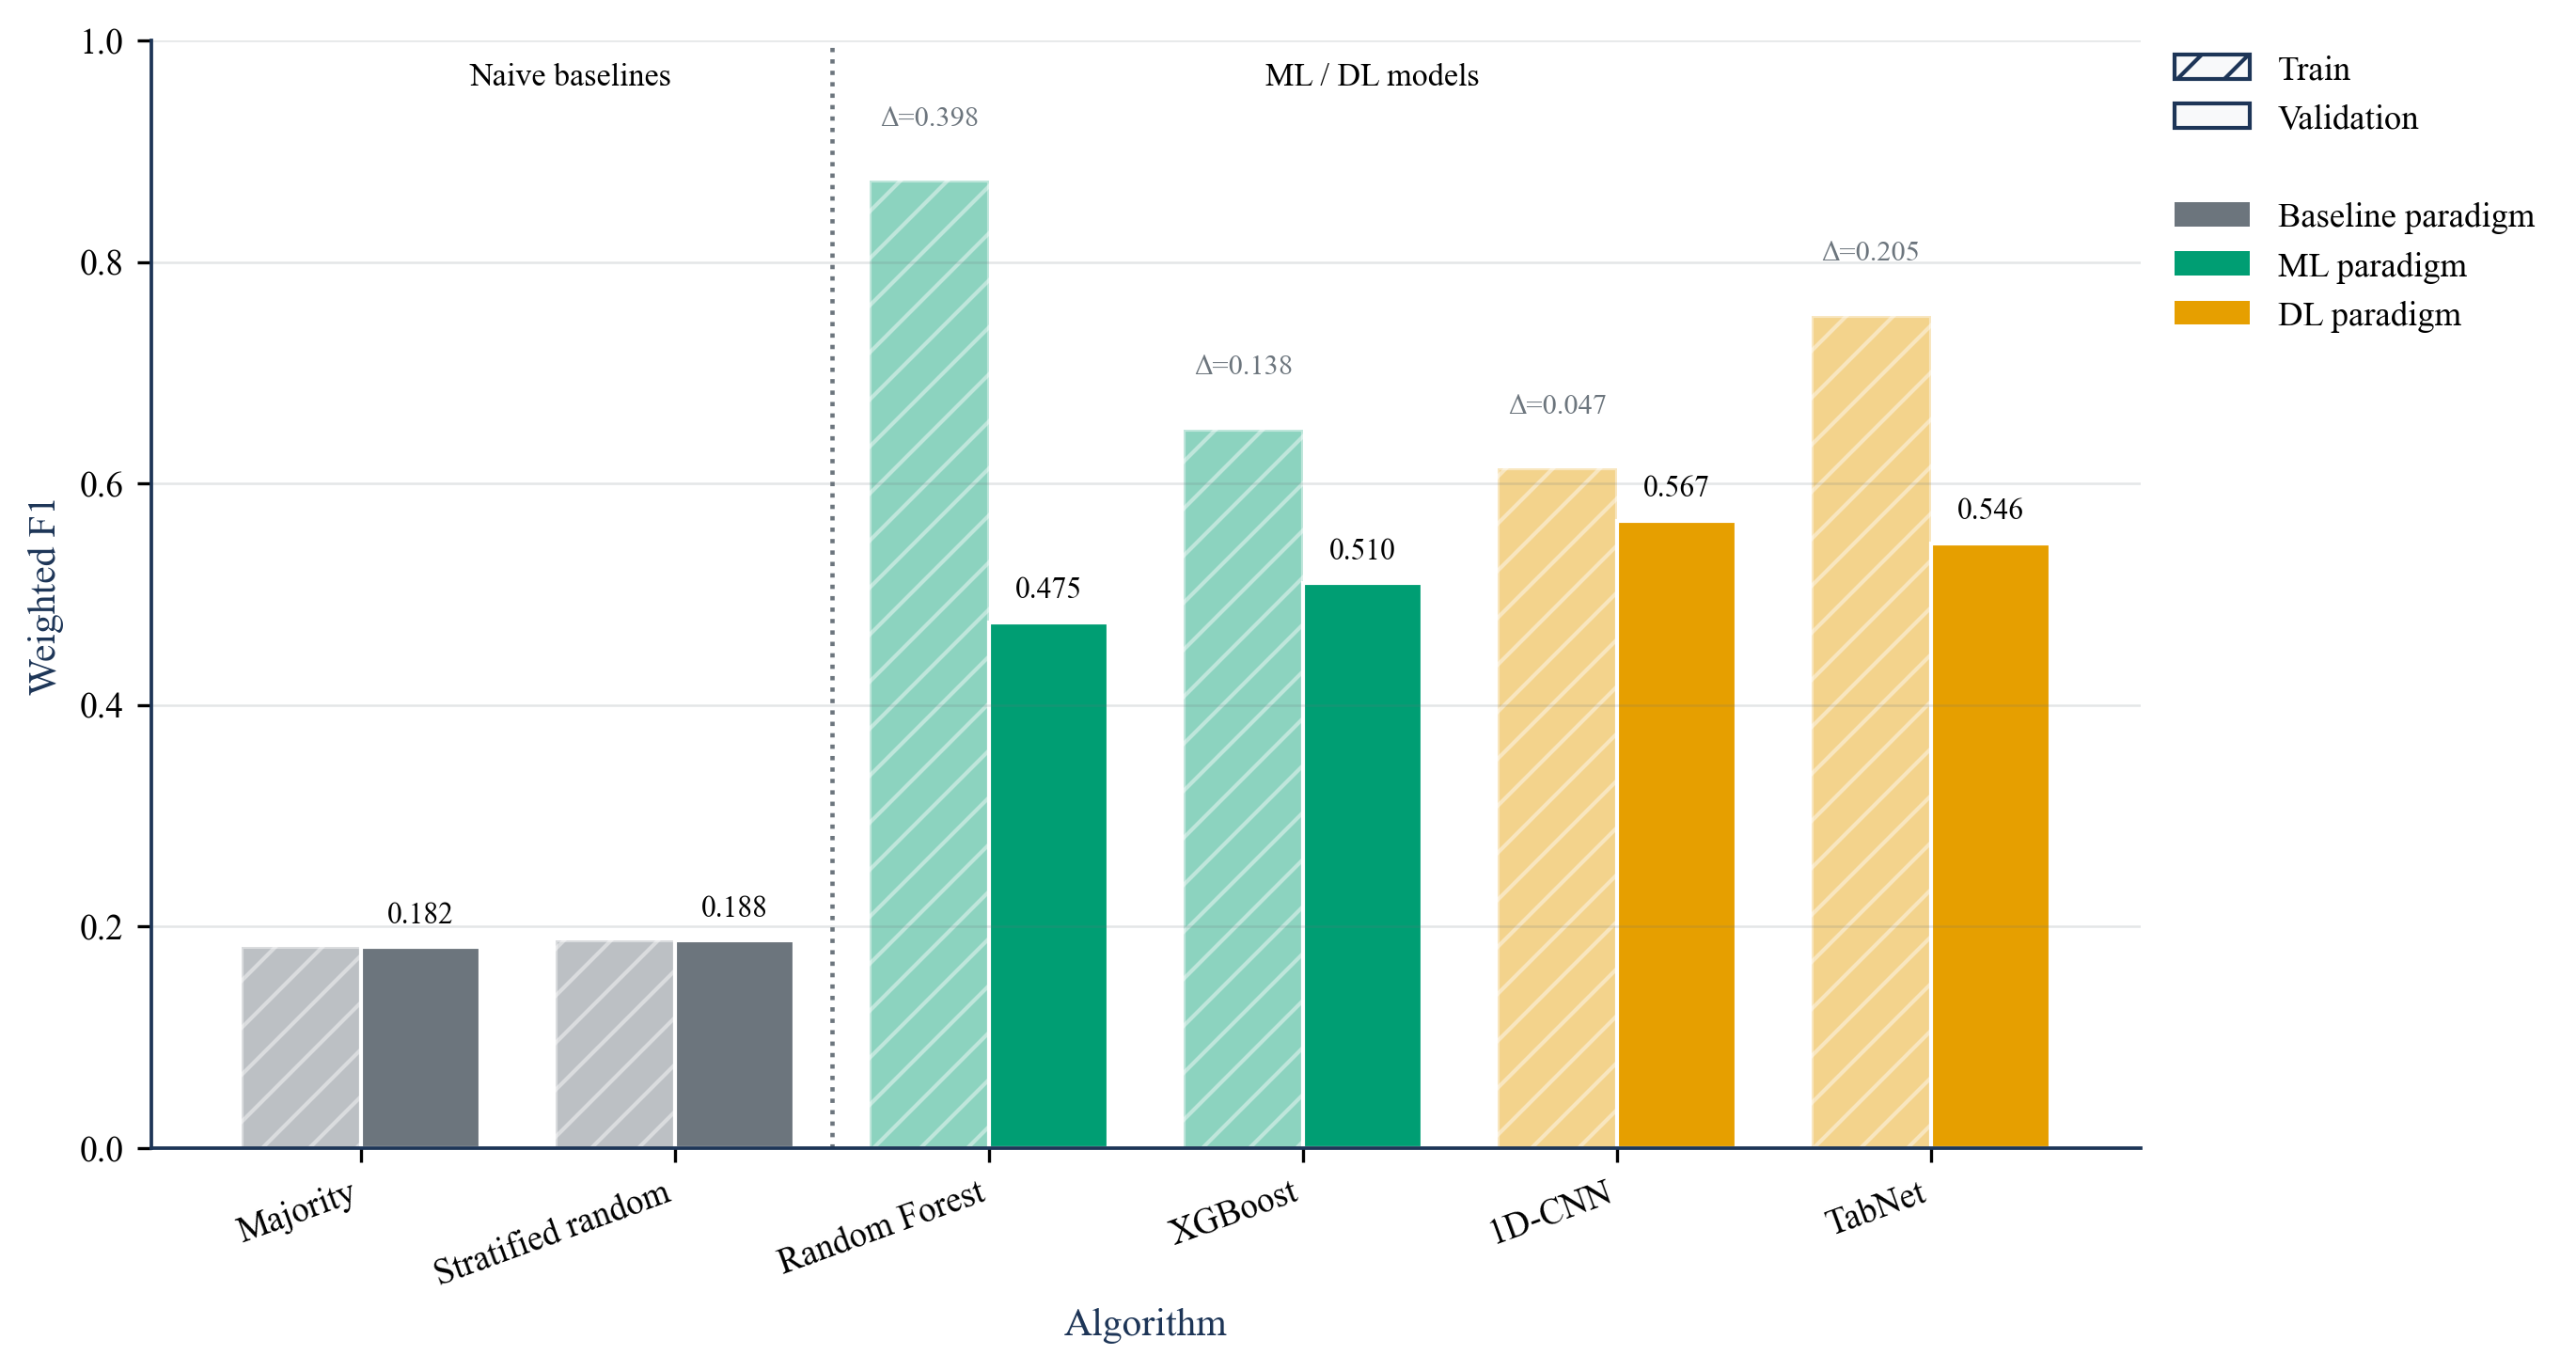
\includegraphics[width=0.88\linewidth,height=0.54\textheight,keepaspectratio]{figures/fig-algorithm-comparison.png}
  \caption{Validation weighted F1 comparison across baseline, ML, and DL algorithms.}
  \label{fig:fig-algorithm-comparison}
\end{figure}

On the held-out Berlin test set, XGBoost achieved weighted F1 = 0.751
{[}95\% confidence interval (CI): 0.749, 0.754{]} (precision = 0.762
{[}0.759, 0.764{]}, recall = 0.752 {[}0.749, 0.754{]}), substantially
outperforming the 1D-CNN (weighted F1 = 0.607 {[}95\% CI: 0.604,
0.611{]}, precision = 0.631 {[}0.624, 0.637{]}, recall = 0.633 {[}0.630,
0.636{]}). Per-genus analysis revealed a performance range from F1 =
0.852 (PLATANUS, best) to F1 = 0.617 (Group 9, worst). Top-tier genera
(F1 \textgreater{} 0.75) included PLATANUS, TILIA, AESCULUS, and Group 1
(conifers). The mid tier (F1 = 0.65-0.75) comprised Group 14, QUERCUS,
CORYLUS, ALNUS, PYRUS, ULMUS, CARPINUS, Group 11, SALIX, FAGUS, and
MALUS. AILANTHUS and Group 9 fell into the low tier (F1 \textless{}
0.65).

Feature importance analysis (\cref{fig:fig-feature-importance}) showed
dominance of summer-month features, with MSI\_07, NDVI\_06, and B3\_06
ranking highest. The top-20 features interleaved vegetation indices
(NDVI, MSI, VARI, EVI, NDWI) and spectral bands (B3, B4, B5, B8A, B11),
with temporal distribution concentrated in June (7 features) and April
(4 features), followed by September (3), July (2), October (2), and May
(1).

\begin{figure}[!htbp]
  \centering
  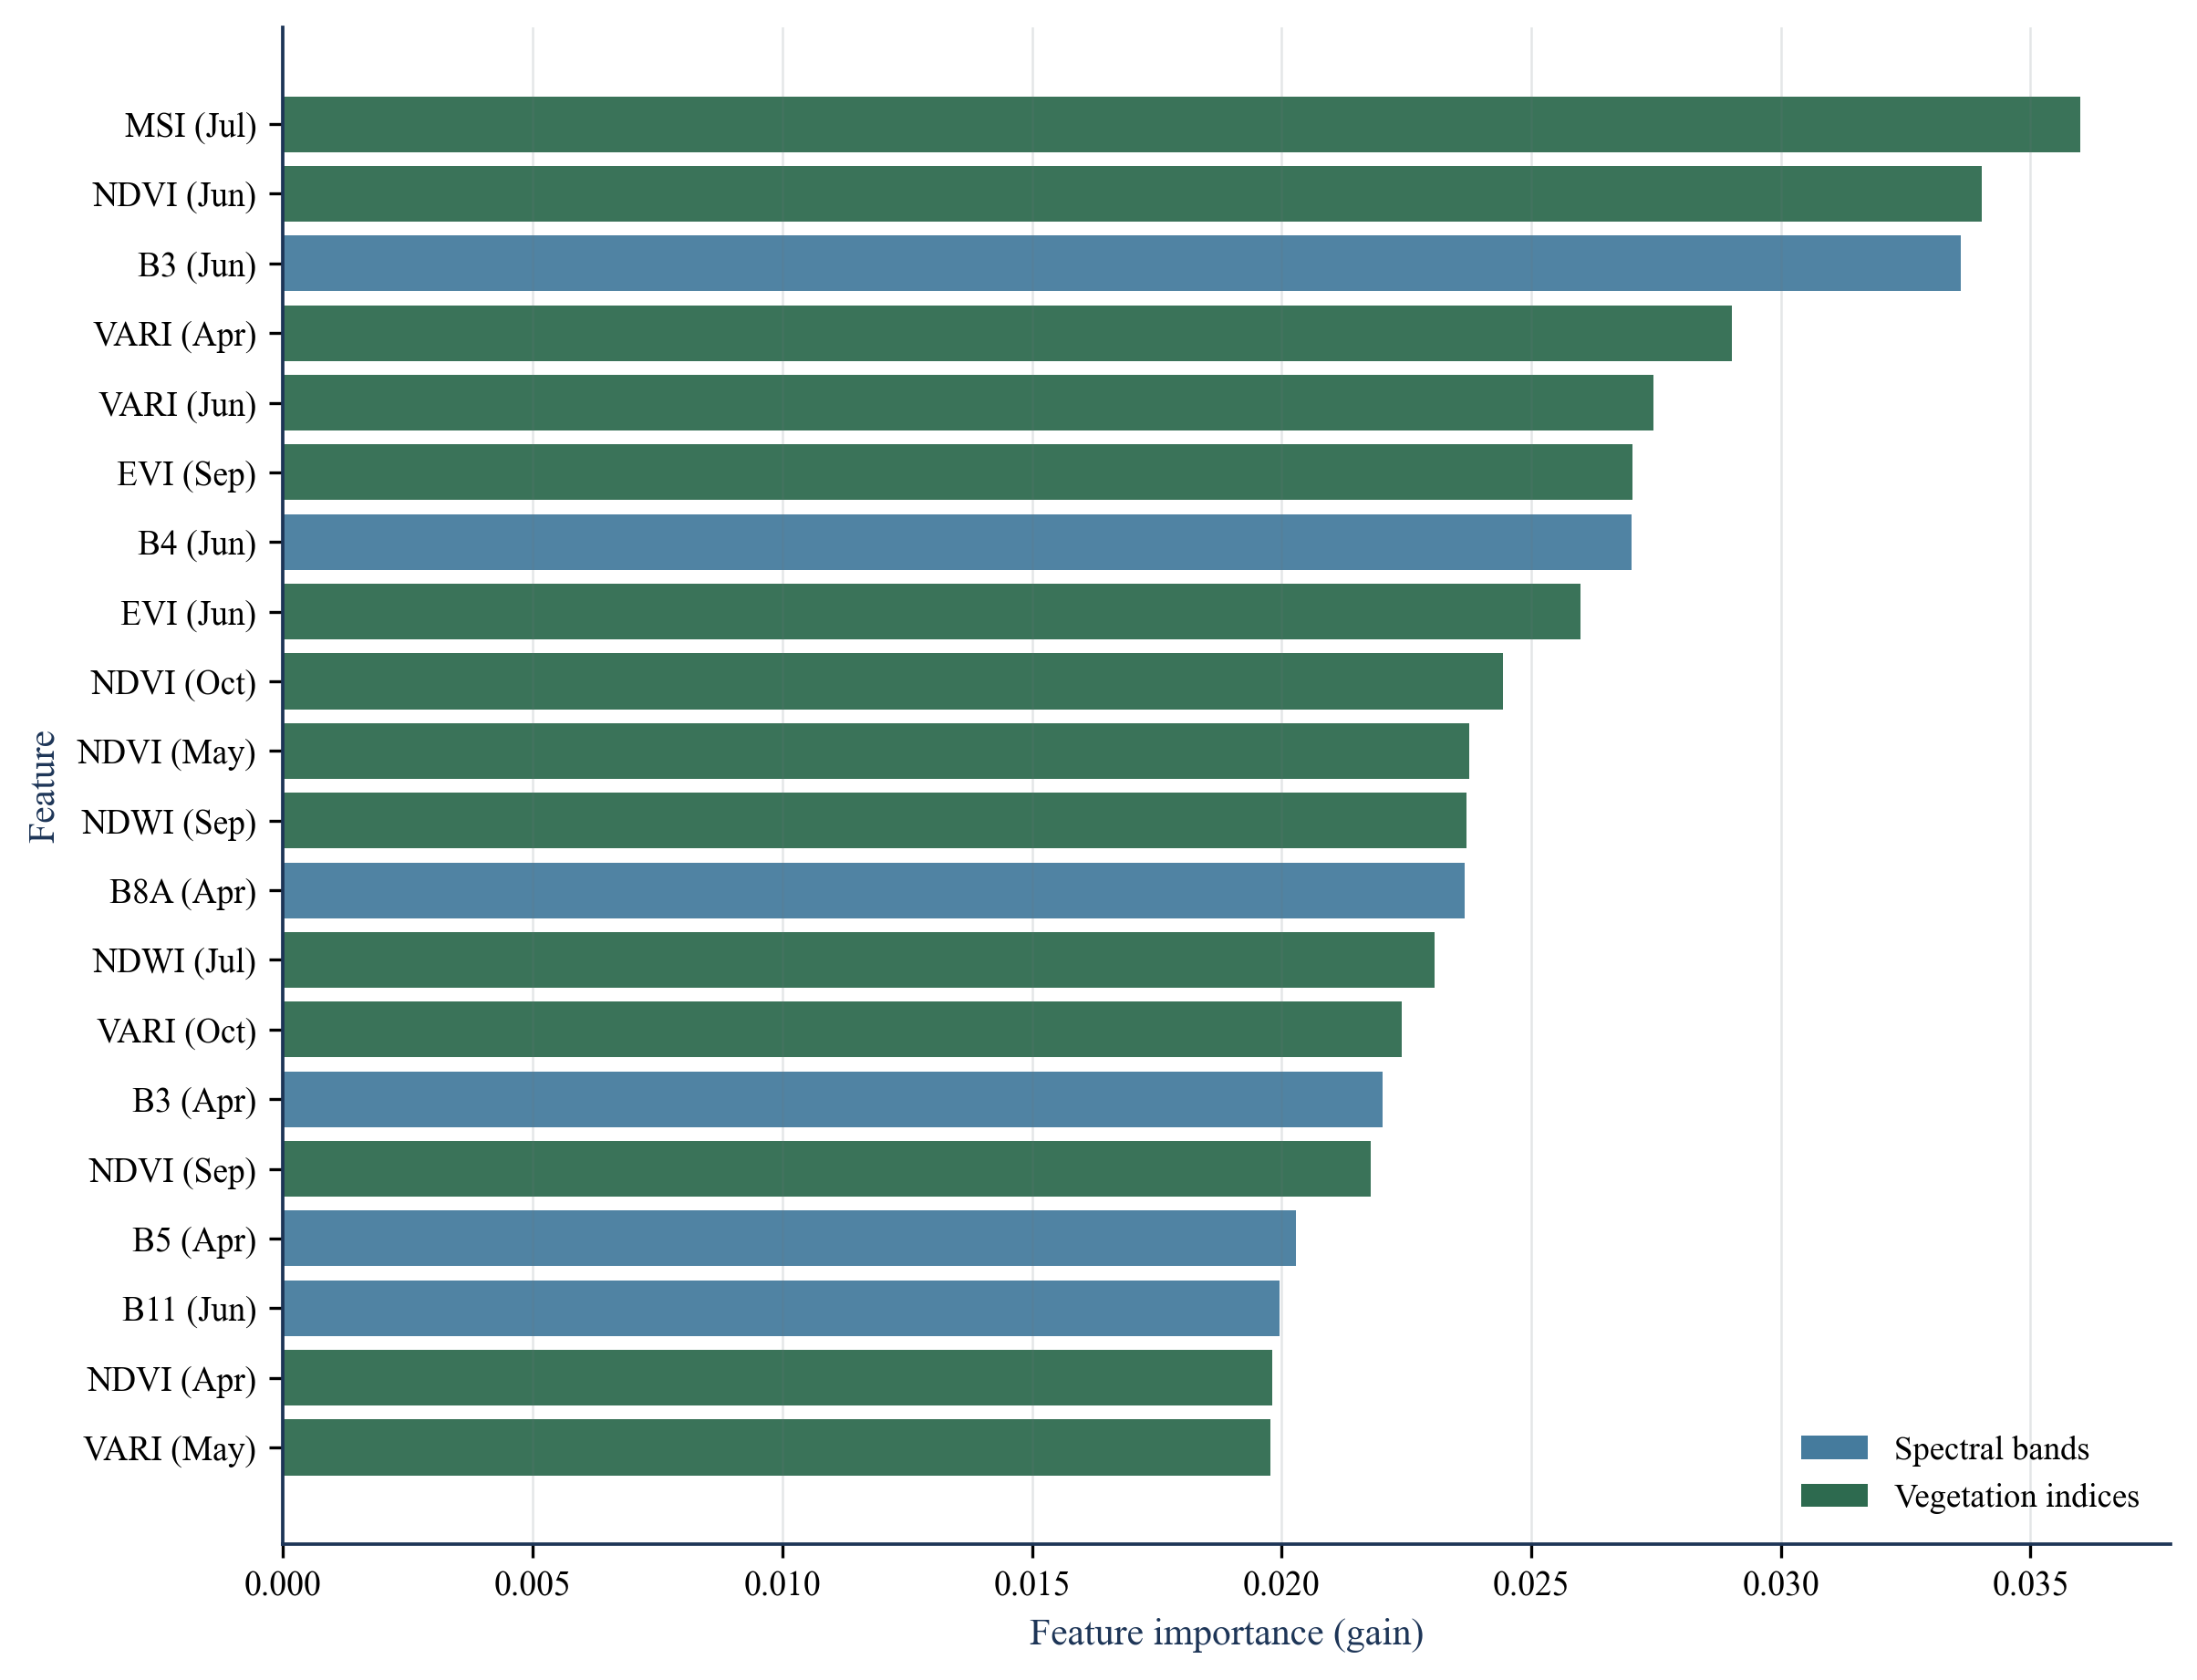
\includegraphics[width=0.85\linewidth,height=0.60\textheight,keepaspectratio]{figures/fig-feature-importance.png}
  \caption{Top-20 XGBoost feature importances.}
  \label{fig:fig-feature-importance}
\end{figure}

Count-based confusion analysis (Appendix,
\cref{fig:fig-confusion-berlin}) identified Group 14 as the primary
source of misclassification, appearing in four of the five most frequent
confusion pairs: Group 14-QUERCUS (2,937 samples), Group 14-Group 11
(1,806), Group 14-TILIA (1,702), and Group 14-Group 1 (1,701). The
TILIA-Group 14 confusion (1,099 samples) was bidirectional, reflecting
shared spectral characteristics between these broad-leaved genera. Group
14, the only class defined by spectral indistinguishability rather than
biological coherence (Section 4.2.1), dominates the confusion matrix,
suggesting that spectrally motivated merging without shared biological
basis produces less stable decision boundaries than biologically
grounded grouping.

\subsection{Zero-Shot Transfer}\label{zero-shot-transfer}

Application of the Berlin-trained models to Leipzig without adaptation
revealed a substantial domain gap (\cref{fig:fig-per-genus-transfer}).
XGBoost dropped from weighted F1 = 0.751 to weighted F1 = 0.377
(absolute drop = 0.374, relative drop = 49.8\%), while the 1D-CNN
dropped from weighted F1 = 0.607 to weighted F1 = 0.380 (absolute drop =
0.227, relative drop = 37.4\%).

Per-genus transfer analysis showed that all 17 classes fell into the
``poor'' category (relative drop \textgreater{} 15\%). The most robust
genera were TILIA (Leipzig F1 = 0.541, relative drop = 35.5\%) and Group
14 (F1 = 0.502, relative drop = 31.7\%), both dominant genera with large
training sample sizes. The most fragile genera were PYRUS (F1 = 0.007),
ULMUS (F1 = 0.009), CORYLUS (F1 = 0.009), and ALNUS (F1 = 0.016),
indicating near-complete failure for rare genera under zero-shot
conditions.

\begin{figure}[!htbp]
  \centering
  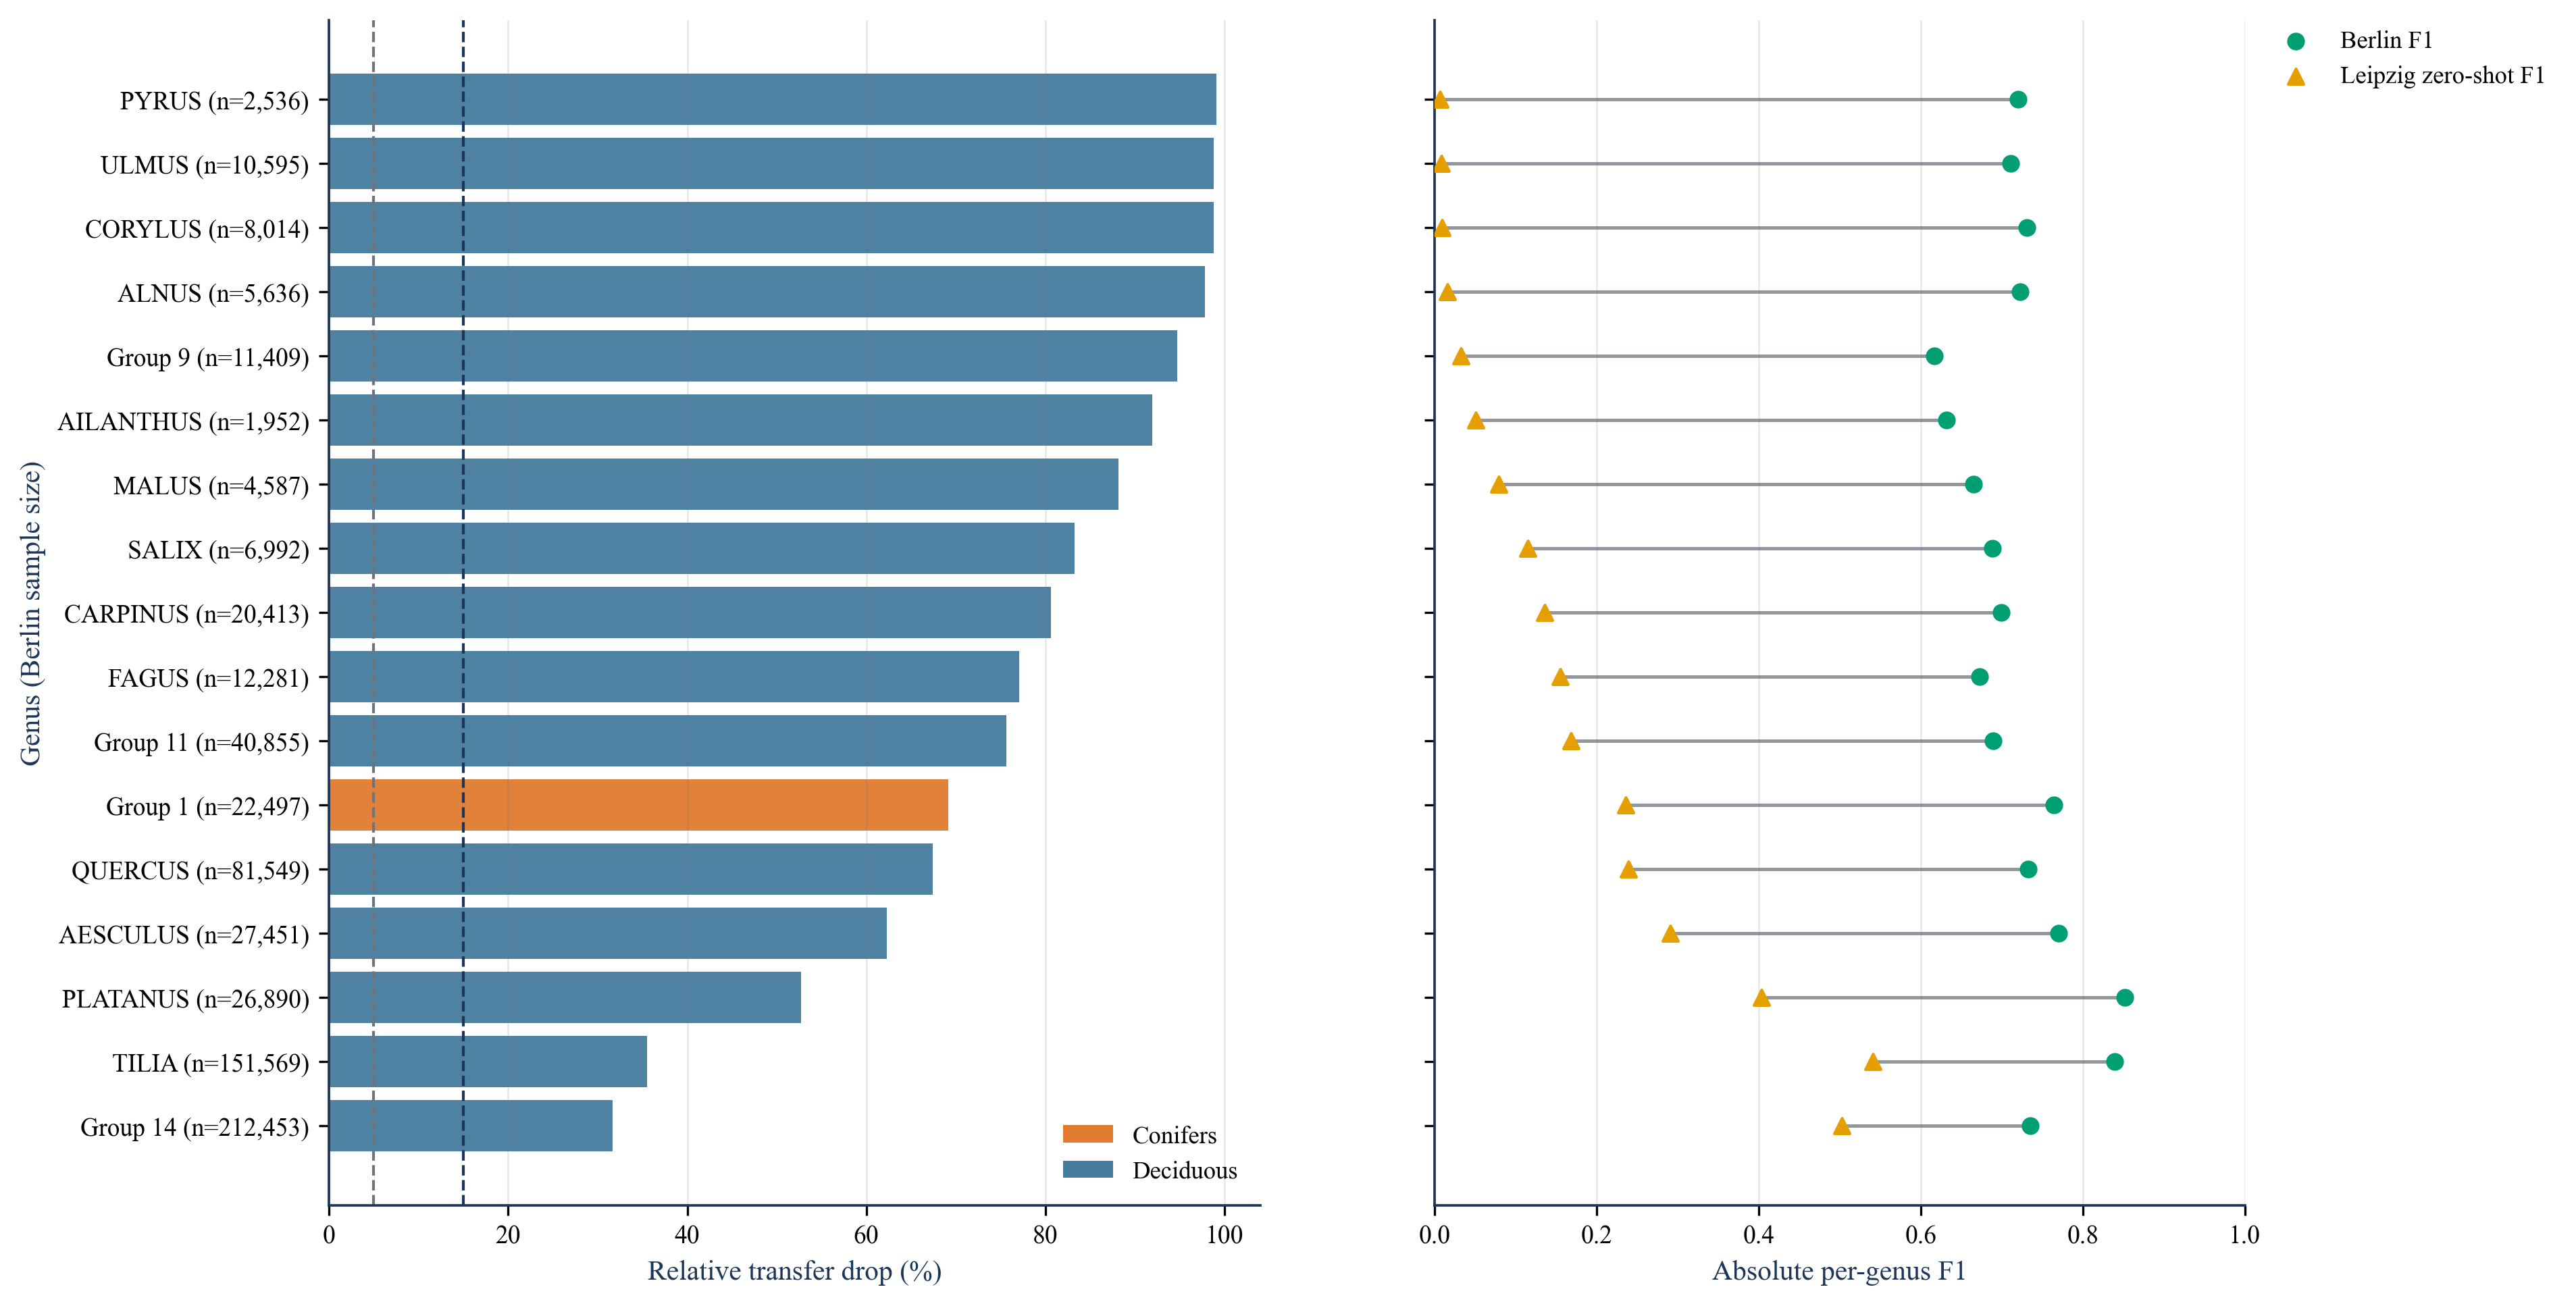
\includegraphics[width=0.90\linewidth,height=0.62\textheight,keepaspectratio]{figures/fig-per-genus-transfer.png}
  \caption{Per-genus relative transfer drop with absolute Berlin and Leipzig F1 side panel.}
  \label{fig:fig-per-genus-transfer}
\end{figure}

\subsection{Hypothesis Tests}\label{hypothesis-tests}

The four a priori hypotheses were tested at α = 0.05
(\cref{tbl:tbl-hypothesis-tests}). H1 (Genus Heterogeneity) was
confirmed: a Kruskal-Wallis test yielded H = 4953.4 (p \textless{}
0.001, η² = 0.163), demonstrating that transfer loss varied
significantly across genera. H2 (Conifer Robustness) remained
inconclusive, as only one conifer group (Group 1) was present in the
dataset, providing insufficient data for the Mann-Whitney U test. H3
(Spectral Separability) was rejected: Spearman rank correlation between
source-domain JM distance and transfer accuracy was negligible (ρ =
−0.132, p = 0.613), indicating that spectral separability in the source
domain does not predict transfer performance. H4 (Fine-Tuning
Efficiency) was rejected at α = 0.05: a positive correlation between
zero-shot transfer gap and fine-tuning data requirements was observed (ρ
= 0.500) but did not reach significance (p = 0.117, n = 17).

\subsection{Fine-Tuning Analysis}\label{fine-tuning-analysis}

Fine-tuning with stratified Leipzig subsets produced divergent recovery
patterns for the two model architectures
(\cref{fig:fig-finetuning-curve}). XGBoost showed consistent gains at
each data fraction: weighted F1 increased from 0.377 (zero-shot) to
0.499 at 10\%, 0.574 at 25\%, 0.662 at 50\%, and 0.771 at 100\% of
Leipzig training data. The recovery trajectory followed a power-law
function with exponent b = 0.194. The 1D-CNN, by contrast, plateaued
from 10\% onward: weighted F1 increased marginally from 0.380
(zero-shot) to 0.450 at 10\% and remained at approximately 0.458 through
25\%, 50\%, and 100\%. This plateau represents a lower bound under the
applied fine-tuning strategy (uniform learning rate at 10\% of the
original, no layer freezing); the CNN fine-tuning results should not be
interpreted as indicative of architectural transfer capacity.

\begin{figure}[!htbp]
  \centering
  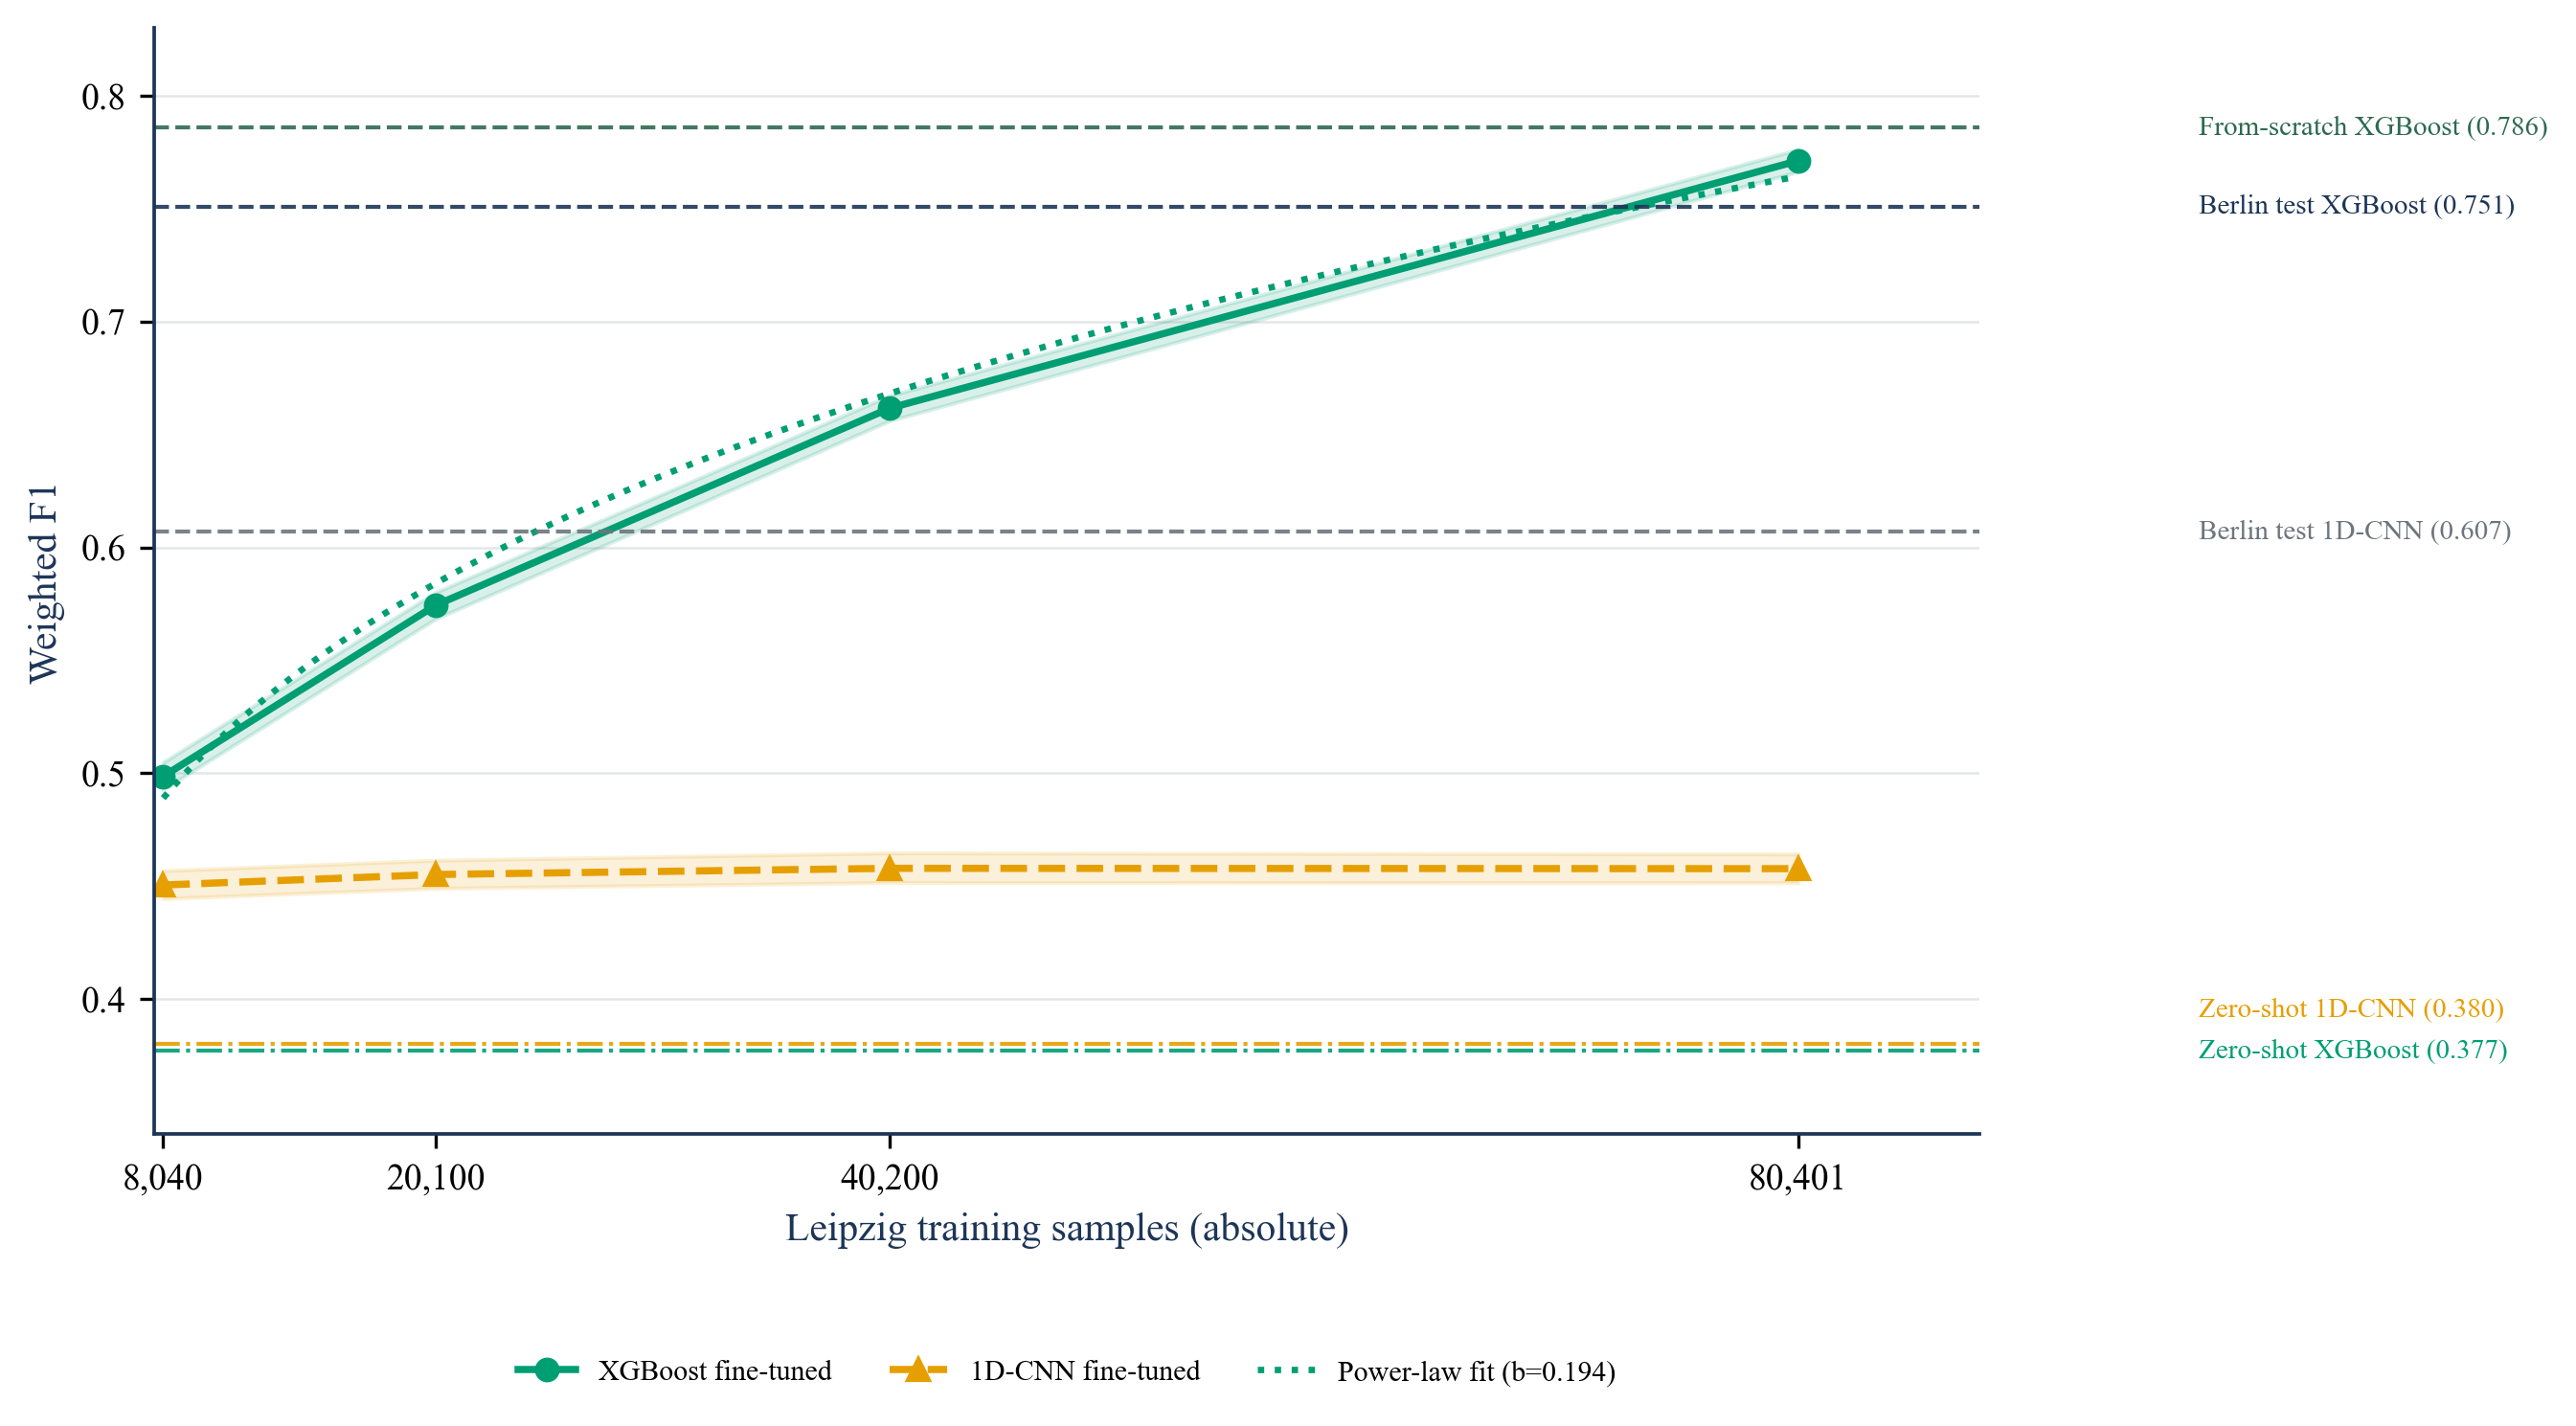
\includegraphics[width=0.90\linewidth,height=0.58\textheight,keepaspectratio]{figures/fig-finetuning-curve.png}
  \caption{Fine-tuning learning curves with inline baseline references and XGBoost power-law fit.}
  \label{fig:fig-finetuning-curve}
\end{figure}

The from-scratch XGBoost baseline, trained exclusively on Leipzig data
with a Leipzig-fitted scaler, achieved weighted F1 = 0.786, slightly
exceeding the fine-tuned model (0.771, −1.5 pp). McNemar's test
confirmed statistically significant differences between fine-tuned and
zero-shot predictions (p \textless{} 0.001) and between fine-tuned and
from-scratch predictions (p \textless{} 0.001). Reaching 90\% of
from-scratch performance (target weighted F1 = 0.707) required the full
100\% of Leipzig training data.

Per-genus recovery patterns (\cref{fig:fig-per-genus-recovery}) varied
widely. The fastest-recovering genera were PLATANUS (F1 from 0.554 at
10\% to 0.856 at 100\%), TILIA (0.624 to 0.835), and AESCULUS (0.458 to
0.801). The slowest-recovering genera were CORYLUS (0.102 to 0.575),
PYRUS (0.135 to 0.575), and ULMUS (0.170 to 0.574). Genera with
near-zero zero-shot F1 exhibited the steepest absolute gains during
fine-tuning but remained the lowest-performing classes at 100\% data
availability.

\begin{figure}[!htbp]
  \centering
  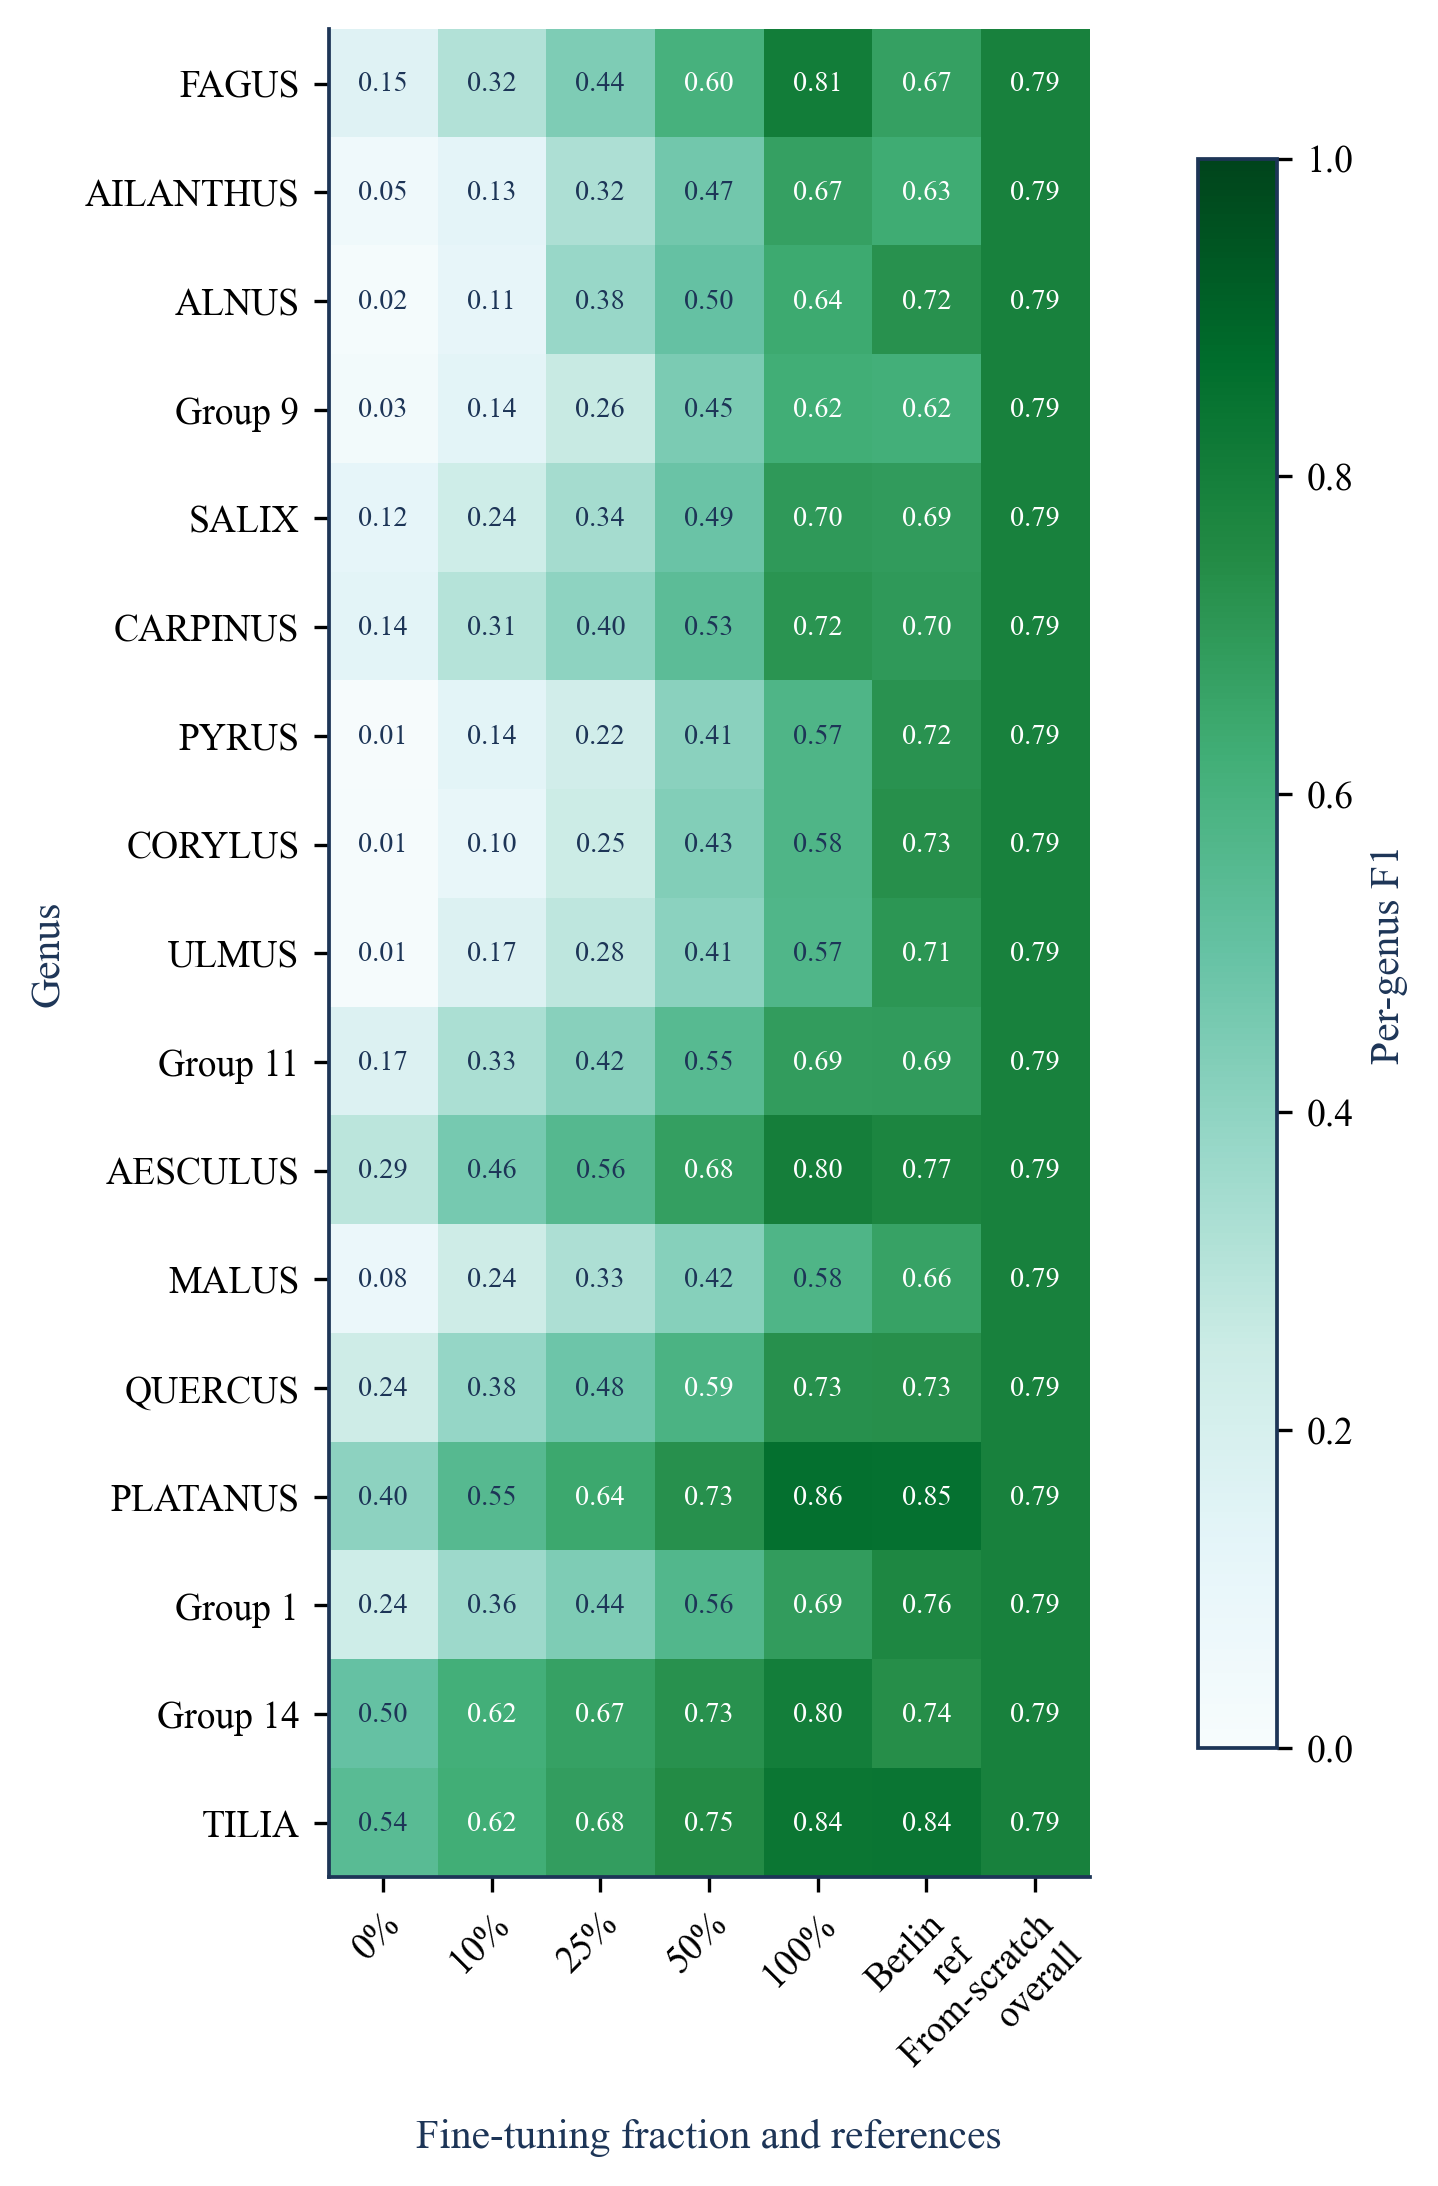
\includegraphics[width=0.90\linewidth,height=0.58\textheight,keepaspectratio]{figures/fig-per-genus-recovery.png}
  \caption{Per-genus fine-tuning recovery heatmap across data fractions.}
  \label{fig:fig-per-genus-recovery}
\end{figure}

\section{Discussion}\label{discussion}

Three aspects structure the discussion: interpretation of the
experimental results against existing benchmarks and methodological
choices (Sections 6.1 to 6.4), practical implications for municipal
cadastre creation (Section 6.5), and limitations constraining
generalisability (Section 6.6).

\subsection{Source-Domain Performance and Benchmark
Comparison}\label{source-domain-performance-and-benchmark-comparison}

XGBoost achieved weighted F1 = 0.751 on the Berlin test set with 17
genus-level classes under spatial block CV with 1200 m blocks. Published
Sentinel-2-only urban benchmarks reach F1 = 0.57-0.66 and OA = 66-89\%
for 10-19 classes (Recanatesi et al. 2025; Zhang et al. 2023; Jiang et
al. 2025), none under spatial block CV; multi-sensor fusion extends to
F1 = 0.72 (Wenger et al. 2024; Yao et al. 2025; Latil et al. 2025) but
remains below the present Sentinel-2-only result. Forest benchmarks at
comparable class counts reach OA = 96\% (Hemmerling et al. 2021),
illustrating the performance gap between closed-canopy and urban
settings. Despite inherent cross-study limitations (Kattenborn et al.
2021), the combination of higher class count, stricter evaluation, and
competitive weighted F1 places the present result above all comparable
benchmarks.

Feature importance analysis reveals summer-month dominance among
XGBoost's top-ranked predictors (MSI\_07, NDVI\_06, B3\_06). MSI
(SWIR1/NIR) captures leaf water content differences (Hunt and Rock
1989), consistent with the known importance of SWIR bands (Immitzer et
al. 2019), while NDVI\_06 captures canopy density at maximum leaf area
and B3\_06 captures chlorophyll-driven reflectance differences. The
combination of these signals indicates that genus discrimination relies
on complementary physiological dimensions.

This summer dominance contrasts with the literature consensus that
spring and autumn are the most discriminative periods (Section 2.2), but
those findings derive from closed-canopy forests where summer canopy
uniformity reduces inter-species contrast. Three factors may explain why
summer carries more weight in the present study: canopy density and Leaf
Area Index (LAI) likely vary more across genera in fragmented settings,
mixed-pixel contamination from non-canopy surfaces is reduced at maximum
canopy closure, and management-driven moisture stress differences may
peak during summer drought. The observed dominance is partly a
consequence of the ML feature selection paradigm (top-50
importance-ranked features favour peak-season magnitudes); the 1D-CNN,
operating on the full temporal sequence, may weight transitional periods
differently.

\subsection{Pipeline Design as Primary Performance
Driver}\label{pipeline-design-as-primary-performance-driver}

Ablation results suggest that the majority of predictive signal
originates from the Sentinel-2 spectral-temporal features themselves,
with hyperparameter optimisation and class distribution information
playing secondary roles. Overall, data quality and preprocessing
decisions contributed more to final performance than algorithm choice or
hyperparameter tuning.

Inverse-frequency sample weighting produced the single largest
performance effect: +18 pp weighted F1 (from 0.571 unbalanced to 0.751
balanced, Berlin test set). This reflects genus frequencies spanning two
orders of magnitude (TILIA \textasciitilde104,000 samples vs.~AILANTHUS
\textasciitilde1,400). Without balancing, rare genera received near-zero
recall (ULMUS 3.6\%, CARPINUS 7.9\%). No comparable study has isolated
this effect: existing approaches range from inverse weighting to
balanced subsets, but none provide a controlled comparison to an
unbalanced baseline (Hemmerling et al. 2021; Rußwurm and Körner 2020;
Yao et al. 2025; Latil et al. 2025), and several studies omit balancing
strategies entirely (Wenger et al. 2024; Jiang et al. 2025; Kollert et
al. 2021). The +18 pp gain represents the first isolated quantification
of class balancing impact in Sentinel-2-based tree classification,
confirming that at factor-100 imbalance, balancing is a primary
performance driver.

The role of CHM contradicts the prevailing literature consensus.
Published CHM gains (+7.1 pp OA to +18.75 pp producer's accuracy;
Section 2.2) derive from richer structural metrics (canopy closure, LAI)
extracted from homogeneous single-site LiDAR or stereo data. The present
study tested only raw canopy height plus two engineered variants
(genus-level percentile rank, within-genus z-score). Under these
conditions, CHM inclusion increased the train-validation gap by +9 to
+14 pp with marginal F1 gains (+0.8 pp maximum), indicating that the
model learns city-specific height artefacts rather than biologically
meaningful patterns. The underlying paradox is that CHM is statistically
genus-discriminative (η² = 0.17 in Welch-ANOVA) yet fails as a
classification feature because urban tree height depends on too many
non-genus factors: site conditions, soil quality, management intensity,
and tree age. CHM exclusion is therefore justified for raw height in
cross-city transfer (Section 6.6).

The evaluation strategy is substantially more conservative than most
comparable work. The 1200 m block size exceeds typical literature
standards of 500 to 800 m, and residual autocorrelation at this distance
remained 0.185 in Berlin and 0.154 in Leipzig, suggesting that reported
F1 values remain slight overestimates. Test evaluation used the
unfiltered dataset under real-world deployment conditions (asymmetric
proximity policy, Section 4.4) and retained all 17 classes, including
the spectrally challenging residual group. Despite these stricter
conditions, Sentinel-2-only performance exceeds multi-sensor fusion
benchmarks.

\subsection{Cross-City Transfer and Algorithmic
Divergence}\label{cross-city-transfer-and-algorithmic-divergence}

The central finding concerns the divergent transfer behaviour of the two
algorithmic paradigms. The 1D-CNN retains 62.6\% of source-domain
weighted F1 under zero-shot conditions versus 50.2\% for XGBoost
(Section 5.2). Source-domain training sample size emerges as a
moderating variable: the two most robust classes (TILIA, Group 14) are
also the two most frequent in Berlin, while rare genera collapse
near-completely, suggesting that small training populations produce
decision boundaries too narrow to survive domain shift. This sample-size
gradient provides a straightforward explanation for the
genus-heterogeneous transfer loss confirmed by H1 (Section 5.3). Group
14, the primary confusion source in Berlin (Section 5.1), exhibits the
second-lowest relative transfer drop. Its broad, spectrally diffuse
decision boundary appears to generalise more readily than the sharper
boundaries of spectrally distinct genera. H2 (conifer robustness) could
not be formally tested with a single conifer group, but Group 1
(PICEA/PINUS) exhibits a transfer drop comparable to the deciduous mean,
which implies that conifer discrimination at 10 m resolution relies on
spectral magnitude differences that shift across cities.

A plausible, though not empirically isolated, explanation lies in
different reliance on spectral versus temporal signal. Feature
importance analysis shows XGBoost's top-ranked features are dominated by
summer-month absolute values (MSI\_07, NDVI\_06, B3\_06), which are
sensitive to domain shift driven by atmospheric conditions and
phenological timing (Tuia et al. 2016). Leaf-out and senescence
dynamics, governed primarily by photoperiod and temperature (Chuine et
al. 2010), may remain more stable across cities within the same climate
zone. The near-perfect cross-city consistency of monthly discriminative
power (Spearman ρ = 0.951; Section 4.2.1) supports this interpretation:
the temporal structure of genus separability is largely city-independent
within the Cfb zone. The 1D-CNN, operating on the full temporal
sequence, may implicitly encode such phenological structure through its
convolutional filters. However, the two paradigms also differ in feature
dimensionality (50 vs.~144 features; Section 4.3.2), so the observed
transfer divergence cannot be attributed solely to temporal encoding. A
controlled ablation (e.g., XGBoost on the full temporal set, 1D-CNN on
reduced features) would be required to isolate the mechanism. This
direct comparison of ML and DL paradigms within the same cross-city
transfer setting has not been reported previously.

Fine-tuning produced divergent recovery patterns: XGBoost followed a
power-law trajectory with consistent gains at each data fraction
(Section 5.4), while the 1D-CNN plateaued from 10\% onward
(\textasciitilde0.458), reflecting suboptimal fine-tuning strategy
(single learning rate, no layer freezing) rather than an architectural
limitation. The paradigm comparison is therefore most informative under
zero-shot conditions, where both models operated on their respectively
optimised configurations; the fine-tuning comparison reflects strategy
limitations rather than fundamental ML-vs-DL differences.

The rejection of H3 (spectral separability predicts transfer accuracy)
is consistent with the sample-size gradient described above:
source-domain JM distance captures between-genus spectral contrast but
not the within-genus decision boundary width that determines transfer
robustness. Genera with high spectral separability but small training
populations (e.g., PYRUS, CORYLUS) still collapse under domain shift,
because their narrow decision boundaries do not generalise. H4 (larger
transfer gap requires more fine-tuning data) showed a positive but
non-significant correlation (ρ = 0.500, p = 0.117). The lack of
significance at n = 17 genera leaves this relationship inconclusive
rather than refuted; the trend is consistent with the observation that
genera with near-zero zero-shot F1 exhibit the steepest absolute gains
during fine-tuning (Section 5.4) but remain the lowest-performing
classes at full data availability.

\subsection{Class Balancing and Transfer
Paradox}\label{class-balancing-and-transfer-paradox}

A revealing side effect of class balancing reveals a counterintuitive
relationship between source-domain optimisation and transfer
performance. Improved balancing increased Berlin performance by +18 pp
while Leipzig zero-shot performance remained flat (\textasciitilde0.38),
increasing the relative transfer drop from -32.5\% to -49.8\%. The most
plausible explanation is that balancing enables finer genus-specific
spectral patterns, including Berlin-specific ones; without it, coarser
majority-class boundaries transfer more readily because they capture
less city-specific detail. Optimising source-domain performance and
transfer robustness are thus competing objectives, a trade-off explored
further in Section 6.5.

\subsection{Implications}\label{implications}

The XGBoost fine-tuning sample-efficiency curve (Section 5.4) translates
directly into municipal fieldwork budgets. For XGBoost, a transfer sweet
spot emerges at 25-50\% of target-city data, where weighted F1 reaches
0.574-0.662; below this range, zero-shot transfer is too unreliable,
while above it, from-scratch training (weighted F1 = 0.786) becomes more
cost-effective. Whether an analogous sweet spot exists for optimised DL
fine-tuning remains open, as the 1D-CNN plateau reflects strategy
limitations rather than architectural constraints (Section 6.3). Robust
genera (TILIA, Group 14) can be mapped with minimal local data, while
fragile genera (PYRUS, ULMUS, CORYLUS) require prioritised local
collection. For single-city applications, XGBoost offers simplicity and
interpretability; for cross-city transfer, the 1D-CNN with a specialised
fine-tuning strategy is the stronger candidate. Combined with existing
tree detection and segmentation pipelines, this framework enables
cost-effective cadastre creation for data-poor cities. The pipeline is
fully replicable, built entirely on freely available data (Sentinel-2
via GEE, municipal cadastres, state survey CHM). Nearly identical
retention rates across cities (91.7\% vs.~91.5\%) confirm
city-independent quality thresholds.

Two concrete optimisation paths require no new data collection. First,
feature strategies preserving temporal continuity (retaining the full
8-month time series for a reduced set of bands and indices rather than
selecting top-N features across all bands) could make ML models more
transferable by giving XGBoost access to the phenological patterns that
currently benefit only the 1D-CNN. Second, transfer-aware class
balancing (weighting by cross-city frequency stability rather than
source-domain frequency alone) could reduce the city-specific
overfitting that class balancing currently amplifies (Section 6.4).
Beyond these, three research directions extend the findings: (a) ML
transfer with domain adaptation (histogram matching, feature-level
alignment) to broaden the transfer sweet spot while preserving XGBoost's
single-city advantage; (b) a multi-city CNN foundation model trained
across climate zones to learn city-independent phenological patterns,
with the long-term vision of a Germany-wide genus classification model;
and (c) richer CHM-derived structural metrics (canopy closure, LAI) from
harmonised LiDAR sources to address the persistent confusion among
spectrally indistinguishable genera such as Group 14, where crown
geometry may provide the discrimination that spectral features cannot.

\subsection{Limitations}\label{limitations}

Several limitations constrain the generalisability of these findings.
The analysis relies on a single year of Sentinel-2 composites (2021),
leaving inter-annual phenological variability unaccounted for. Both
study areas share the same Köppen climate zone (Cfb); transfer behaviour
to climatically distinct regions remains untested. The classification
operates at genus level with a per-tree point extraction approach that
exploits no spatial context such as crown shape or neighbourhood
composition.

Cadastre records were used as provided by municipal authorities without
independent verification of genus labels, positional accuracy, or record
currency; label noise from misclassified or outdated entries propagates
into training data. However, several pipeline steps provide indirect
evidence for acceptable data quality: snap-to-peak correction with
CHM-based filtering excluded entries lacking a detectable canopy, the
NDVI plausibility check removed spectrally implausible locations, and
the subsequent outlier analysis identified only a small fraction of
spectral outliers (4.1\%), whose removal produced no measurable training
improvement. The latter finding suggests that flagged samples largely
reflect natural within-genus spectral variability rather than labelling
errors. Differential label quality between the two cadastres could
conflate label noise with true spectral domain shift, inflating or
deflating the measured transfer gap depending on which city maintains
cleaner records. CHM processing derived only raw canopy height and two
normalised variants; richer structural features such as crown area,
crown volume, or canopy closure were not extracted from the rasterised
CHM product, although such metrics could provide additional genus
discrimination, particularly for spectrally similar classes.

The sequential ablation design means that later decisions (e.g., feature
selection) were conditioned on earlier ones (e.g., CHM exclusion); joint
or factorial optimisation could yield different configurations. All
pipeline decisions, including feature selection, quality thresholds, and
class grouping, were made on Berlin data and applied unchanged to
Leipzig. The study quantified the resulting transfer gap but did not
optimise for cross-city transfer; the observed performance therefore
represents a lower bound under a ``no target knowledge'' scenario.
Google Colab resource limits constrained hyperparameter search depth (40
trials for XGBoost, 20 for the 1D-CNN) and prevented exhaustive
architecture exploration. A single random seed was used throughout;
stochastic variation across seeds was not quantified.

The transfer evaluation relies on a single city pair. The
spectral-versus-temporal transfer thesis is supported by convergent
evidence but was not isolated through a controlled feature ablation.
Fine-tuning tested only four data fractions (10\%, 25\%, 50\%, 100\%),
leaving the 0-10\% recovery curve uncharted, and the power-law fit is
overparameterised for four data points. A from-scratch 1D-CNN baseline
was not trained due to resource constraints, preventing a complete
transfer-advantage comparison across paradigms. The Berlin-fitted
feature scaler was retained during fine-tuning; refitting on Leipzig
statistics could improve target-domain feature distributions. The
expected effect direction is a conservative bias: Berlin-derived scaling
parameters compress Leipzig features toward Berlin's distribution
centre, potentially suppressing city-specific discriminative variation
and producing an underestimate of achievable fine-tuning performance.

\section{Conclusion}\label{conclusion}

This study addresses the question of whether Sentinel-2-based genus
classification models trained on a data-rich city can transfer to a
data-poor city, and how much local data is required to recover
acceptable performance. The resulting baseline, covering 17 genus-level
classes across Berlin and Leipzig with two algorithmic paradigms and
three sequential experiments, provides the first systematic empirical
answer for freely available satellite data.

Three overarching findings structure the contribution. First, pipeline
design contributes more to classification performance than algorithm
selection or hyperparameter tuning. Class balancing, spatial evaluation
strategy, and feature engineering collectively determine the performance
range within which algorithmic choices operate. Second, the 1D-CNN
retains more source-domain performance under zero-shot conditions than
XGBoost. A plausible explanation is that convolutional encoding of
phenological dynamics transfers more effectively than reliance on
peak-season spectral values, though the confounded feature
dimensionality (50 vs.~144 features) prevents definitive attribution.
This divergence nevertheless identifies temporal representation as a
promising lever for improving cross-city generalisability. Third, for
XGBoost, a practical transfer sweet spot exists at moderate amounts of
local target data, where transferred models recover substantial
performance; beyond this range, from-scratch training on local data
alone becomes competitive. Whether this pattern extends to optimised DL
fine-tuning strategies remains to be established. This relationship
translates directly into municipal fieldwork budgets for cities planning
cadastre creation with limited resources.

Two additional insights refine these findings. Source-domain
optimisation and transfer robustness are partially competing objectives:
improved class balancing sharpens genus-specific decision boundaries
that generalise less readily across domains. Transfer robustness varies
systematically across genera, with training sample size rather than
spectral separability emerging as the primary moderating variable, a
result that reinterprets transfer failure as a data-availability problem
rather than a spectral-similarity problem.

The study contributes a fully reproducible, end-to-end pipeline built
entirely on open data sources (Sentinel-2 via GEE, municipal tree
cadastres, state survey CHM), with a-priori hypothesis formulation as a
safeguard against post-hoc interpretation bias. The evaluation protocol,
employing spatial block CV with conservatively sized blocks, asymmetric
proximity filtering, and unfiltered test data reflecting deployment
conditions, provides a methodological template for future transfer
studies. Source-domain performance under these strict conditions exceeds
published Sentinel-2-only and multi-sensor fusion benchmarks, confirming
that rigorous evaluation and competitive accuracy are not mutually
exclusive.

Three research directions extend these findings. First, expanding the
evaluation to additional city pairs across different climate zones would
test whether the observed transfer patterns generalise beyond
climatically similar cities; multi-year composites would further reduce
single-year phenological bias. Second, domain adaptation techniques and
optimised neural network fine-tuning strategies (layer freezing,
progressive unfreezing) could actively close the transfer gap rather
than merely quantifying it, potentially broadening the transfer sweet
spot identified here. Third, multi-pixel crown sampling and richer
structural features from harmonised LiDAR sources could address the
persistent confusion among spectrally indistinguishable genera that
spectral features alone cannot resolve.

Combined with existing tree detection and segmentation algorithms, the
framework established here provides a foundation for cost-effective,
fully automated cadastre creation in data-poor cities.

\FloatBarrier
\clearpage
\appendix

\section{Appendix}\label{appendix}

\subsection{Hypothesis Test Summary}\label{hypothesis-test-summary}

\begin{table}[!htbp]
  \centering
  \small
  \caption{Summary of four a-priori hypothesis tests.}
  \label{tbl:tbl-hypothesis-tests}
  \begin{adjustbox}{max width=\linewidth}
  \begin{tabularx}{\linewidth}{>{\raggedright\arraybackslash}X>{\raggedright\arraybackslash}X>{\raggedright\arraybackslash}X>{\raggedright\arraybackslash}X>{\raggedright\arraybackslash}X>{\raggedright\arraybackslash}X>{\raggedright\arraybackslash}X}
  \toprule
  Hypothesis & Statement & Test & Statistic & p-value & Effect Size & Result \\
  \midrule
  H1 & Transfer loss varies significantly across genera & Kruskal-Wallis H & H = 4953.4 & <0.001 & eta-squared = 0.163 & Confirmed \\
  H2 & Evergreen genera exhibit smaller transfer losses & Mann-Whitney U & -- & -- & -- & Inconclusive (n=1 conifer group) \\
  H3 & Higher JM-distance predicts higher transfer accuracy & Spearman rho & rho = -0.132 & 0.613 & -- & Rejected \\
  H4 & Larger zero-shot gap requires more FT data for recovery & Spearman rho & rho = 0.500 & 0.117 & -- & Rejected (positive trend, not significant at alpha = 0.05) \\
  \bottomrule
  \end{tabularx}
  \end{adjustbox}
\end{table}

\subsection{Feature List (147
Features)}\label{feature-list-147-features}

\emph{Spectral Bands (64 features: 8 bands x 8 months,
April--November):}

B2\_04, B2\_05, B2\_06, B2\_07, B2\_08, B2\_09, B2\_10, B2\_11, B3\_04,
B3\_05, B3\_06, B3\_07, B3\_08, B3\_09, B3\_10, B3\_11, B4\_04, B4\_05,
B4\_06, B4\_07, B4\_08, B4\_09, B4\_10, B4\_11, B5\_04, B5\_05, B5\_06,
B5\_07, B5\_08, B5\_09, B5\_10, B5\_11, B8\_04, B8\_05, B8\_06, B8\_07,
B8\_08, B8\_09, B8\_10, B8\_11, B8A04, B8A05, B8A06, B8A07, B8A08,
B8A09, B8A10, B8A11, B11\_04, B11\_05, B11\_06, B11\_07, B11\_08,
B11\_09, B11\_10, B11\_11, B12\_04, B12\_05, B12\_06, B12\_07, B12\_08,
B12\_09, B12\_10, B12\_11

\emph{Vegetation Indices (80 features: 10 indices x 8 months,
April--November):}

CIre04, CIre05, CIre06, CIre07, CIre08, CIre09, CIre10, CIre11, EVI04,
EVI05, EVI06, EVI07, EVI08, EVI09, EVI10, EVI11, IRECI04, IRECI05,
IRECI06, IRECI07, IRECI08, IRECI09, IRECI10, IRECI11, MSI04, MSI05,
MSI06, MSI07, MSI08, MSI09, MSI10, MSI11, NDVI04, NDVI05, NDVI06,
NDVI07, NDVI08, NDVI09, NDVI10, NDVI11, NDVIre04, NDVIre05, NDVIre06,
NDVIre07, NDVIre08, NDVIre09, NDVIre10, NDVIre11, NDWI04, NDWI05,
NDWI06, NDWI07, NDWI08, NDWI09, NDWI10, NDWI11, NDre1\_04, NDre1\_05,
NDre1\_06, NDre1\_07, NDre1\_08, NDre1\_09, NDre1\_10, NDre1\_11,
RTVIcore04, RTVIcore05, RTVIcore06, RTVIcore07, RTVIcore08, RTVIcore09,
RTVIcore10, RTVIcore11, VARI04, VARI05, VARI06, VARI07, VARI08, VARI09,
VARI10, VARI11

\emph{CHM (3 features):}

CHM\_1m, CHM1m\_percentile, CHM1m\_zscore

\subsection{Supplementary Confusion
Matrices}\label{supplementary-confusion-matrices}

Supplementary confusion matrices are provided with the shared 17-class
label set from Section 4.2. \cref{fig:fig-confusion-berlin} reports
Berlin XGBoost confusion in absolute counts,
\cref{fig:fig-confusion-berlin-xgb} reports the corresponding normalized
Berlin XGBoost matrix, and \cref{fig:fig-confusion-leipzig-zeroshot}
reports normalized Leipzig zero-shot XGBoost confusion.

\begin{figure}[!htbp]
  \centering
  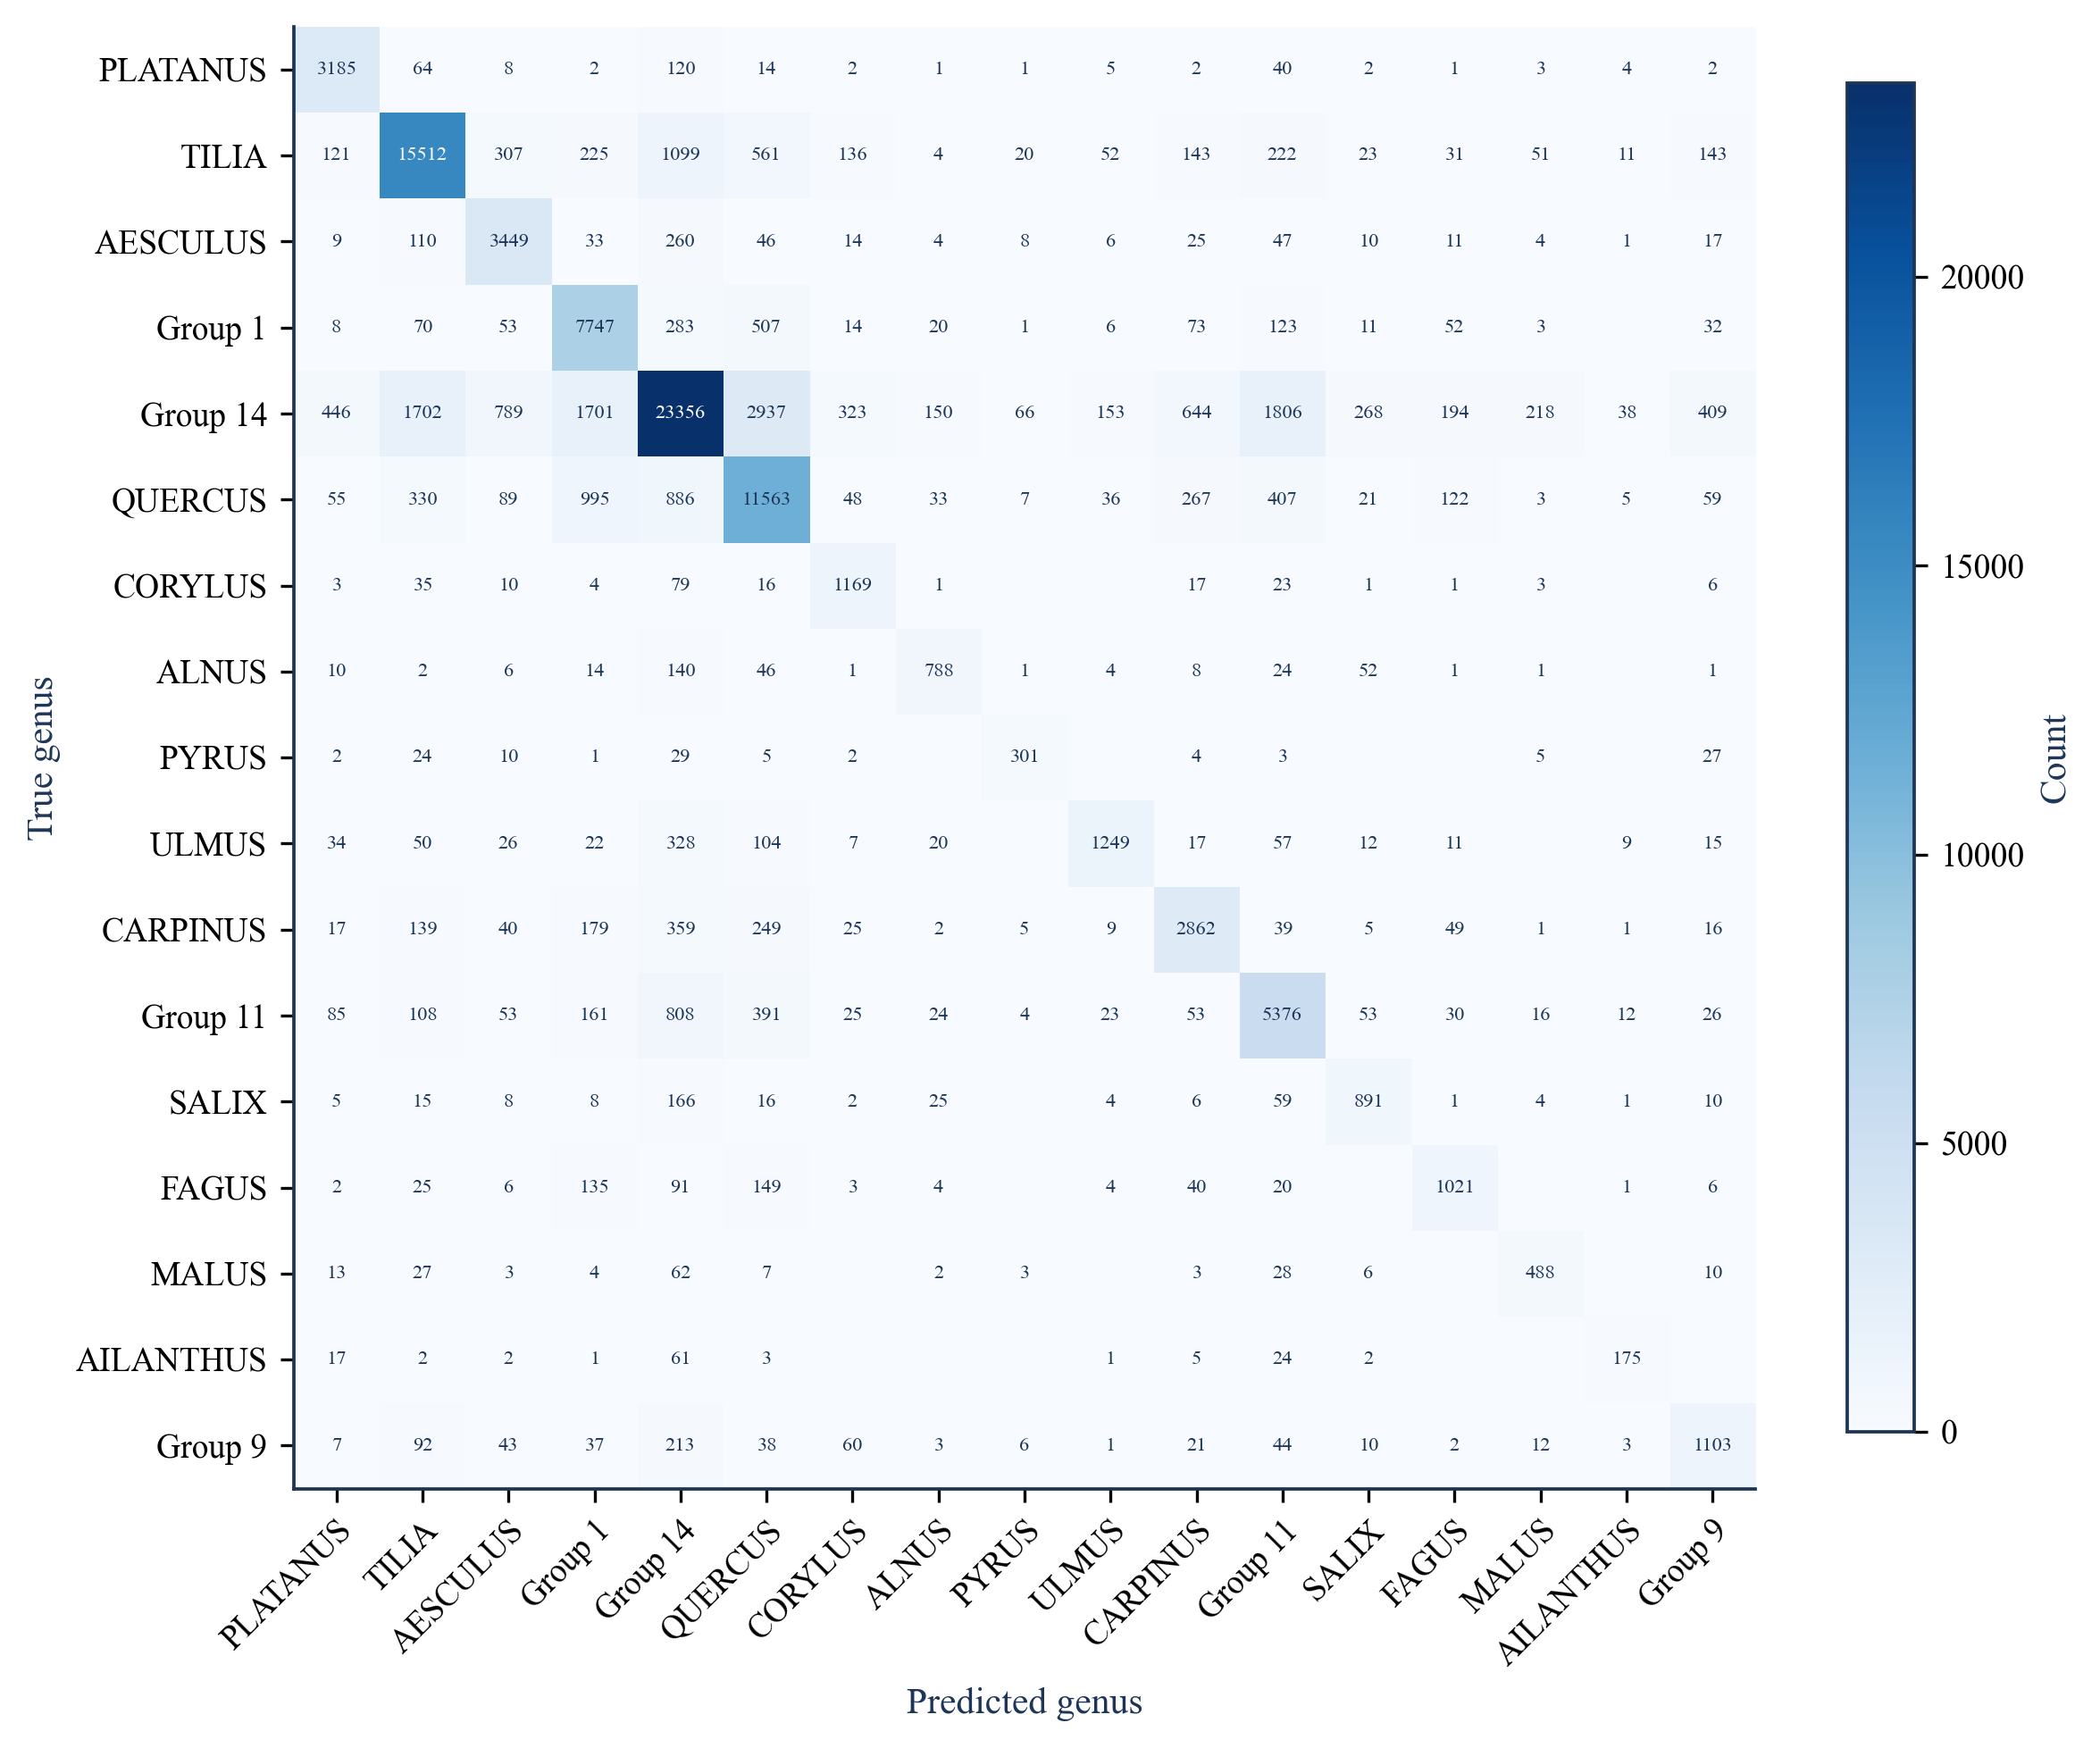
\includegraphics[width=0.90\linewidth,height=0.62\textheight,keepaspectratio]{figures/fig-confusion-berlin.png}
  \caption{Berlin confusion matrix in absolute counts (17 classes), ordered by per-class Berlin F1.}
  \label{fig:fig-confusion-berlin}
\end{figure}

\begin{figure}[!htbp]
  \centering
  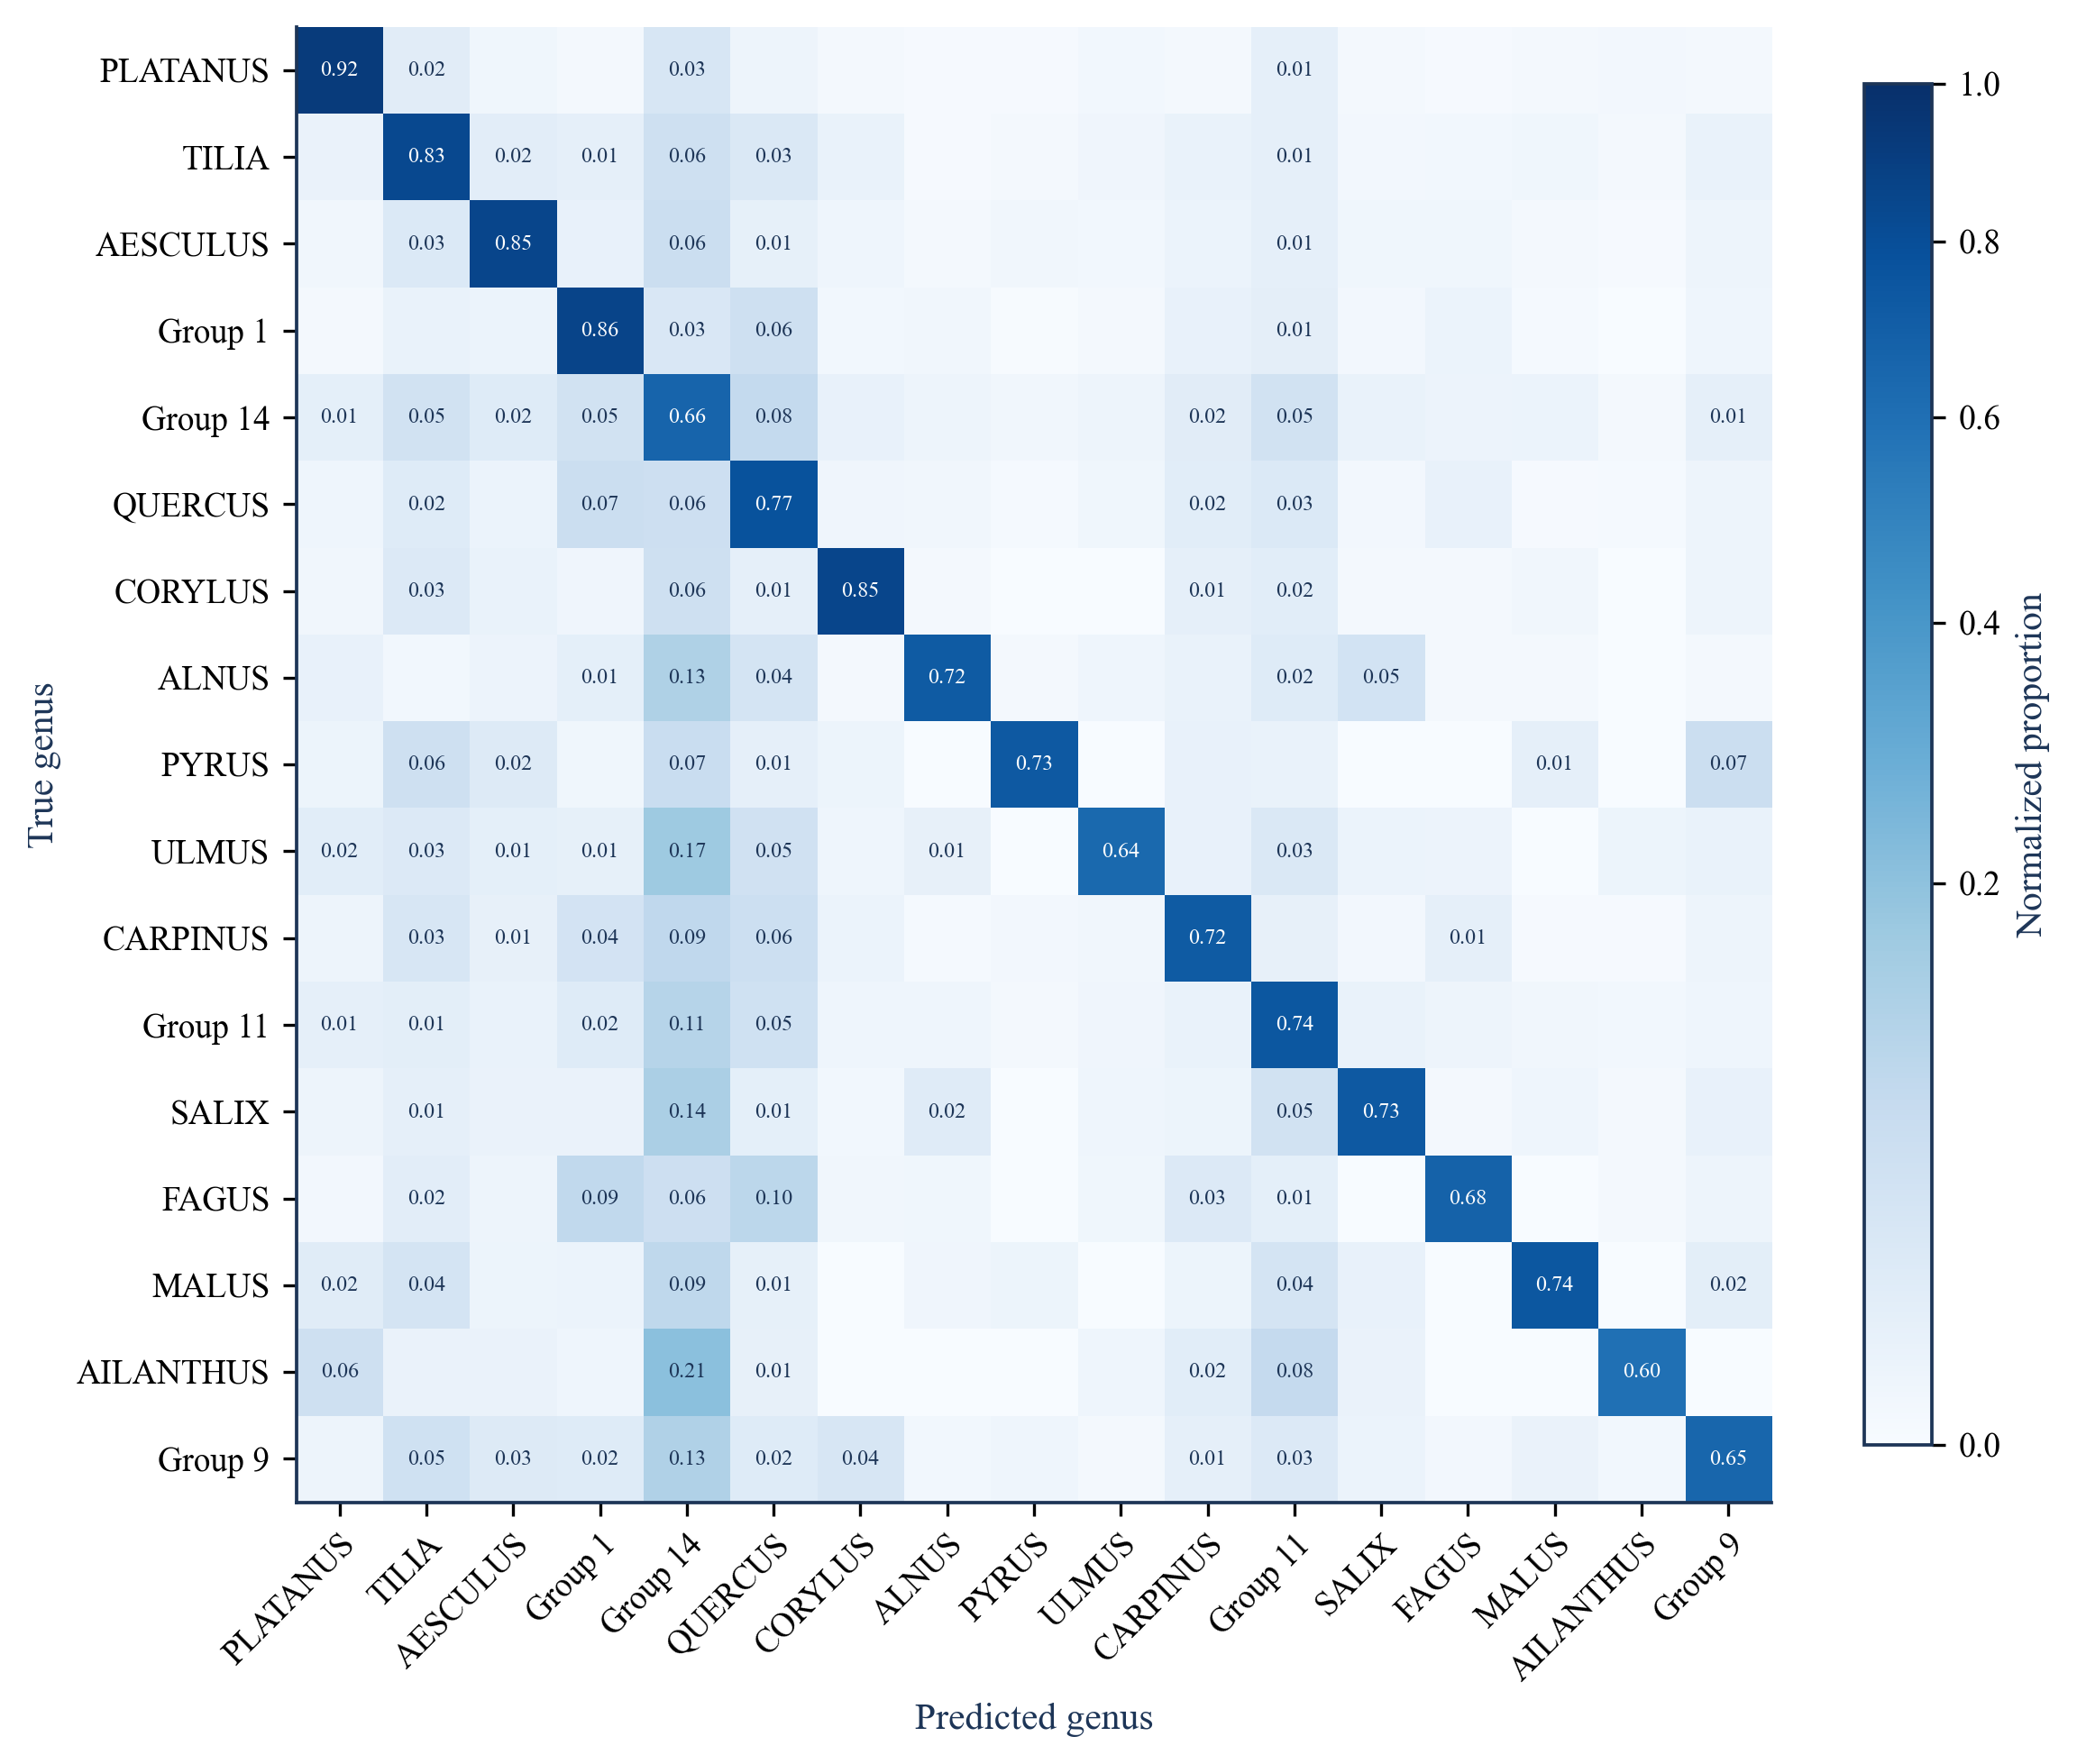
\includegraphics[width=0.95\linewidth,height=0.70\textheight,keepaspectratio]{figures/fig-confusion-berlin-xgb.png}
  \caption{Appendix A.2 normalized confusion matrix for Berlin XGBoost.}
  \label{fig:fig-confusion-berlin-xgb}
\end{figure}

\begin{figure}[!htbp]
  \centering
  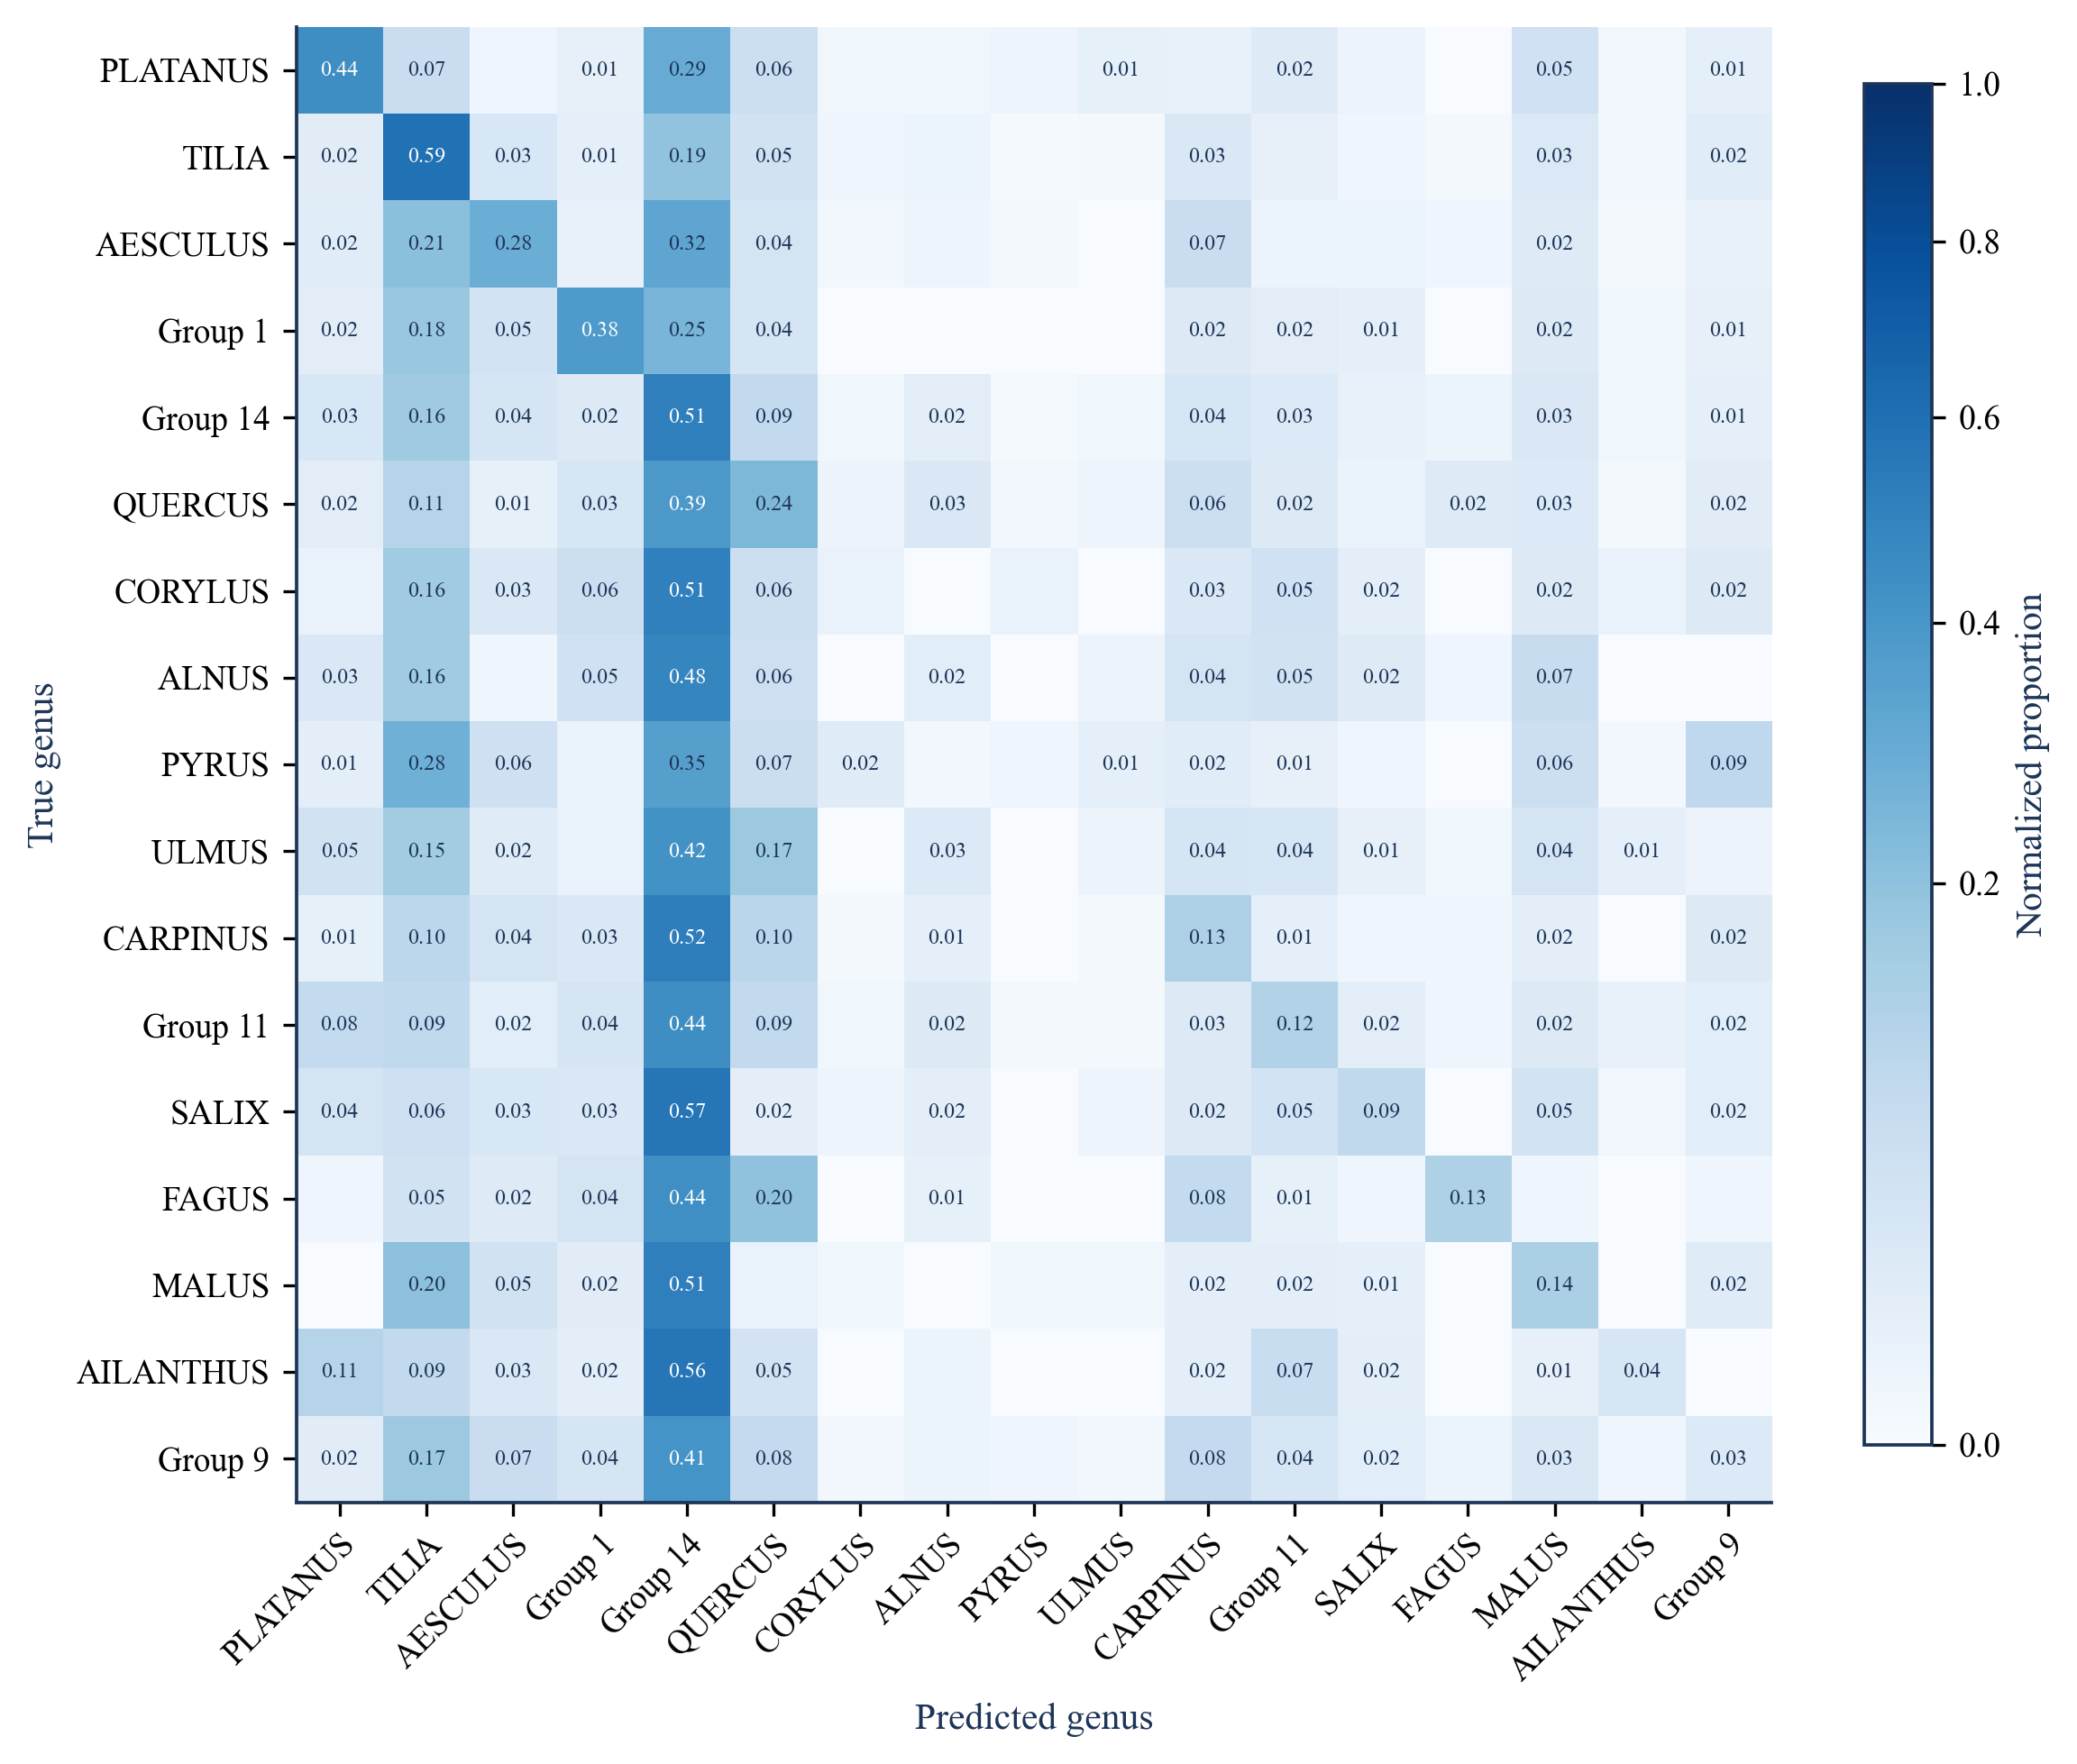
\includegraphics[width=0.95\linewidth,height=0.70\textheight,keepaspectratio]{figures/fig-confusion-leipzig-zeroshot.png}
  \caption{Appendix A.3 normalized confusion matrix for Leipzig zero-shot XGBoost.}
  \label{fig:fig-confusion-leipzig-zeroshot}
\end{figure}

\FloatBarrier
\clearpage

\subsection{Hyperparameter
Configurations}\label{hyperparameter-configurations}

\emph{XGBoost (Optuna, Tree-structured Parzen Estimator (TPE) sampler,
MedianPruner, 40 trials on 100k subset):}

\begin{table}[!htbp]
  \centering
  \small
  \caption{Final XGBoost hyperparameter configuration selected from Optuna tuning.}
  \label{tbl:tbl-hyperparams-xgboost}
  \begin{adjustbox}{max width=\linewidth}
  \begin{tabularx}{\linewidth}{>{\raggedright\arraybackslash}X>{\raggedright\arraybackslash}X}
  \toprule
  Parameter & Value \\
  \midrule
  max\_depth & 12 \\
  learning\_rate & 0.0542 \\
  n\_estimators & 358 \\
  subsample & 0.851 \\
  colsample\_bytree & 0.905 \\
  min\_child\_weight & 2 \\
  reg\_alpha & 0.0765 \\
  reg\_lambda & 1.358 \\
  \bottomrule
  \end{tabularx}
  \end{adjustbox}
\end{table}

\emph{1D-CNN (Optuna, 20 trials on 100k subset):}

\begin{table}[!htbp]
  \centering
  \small
  \caption{Final 1D-CNN training and optimisation configuration selected from Optuna tuning.}
  \label{tbl:tbl-hyperparams-cnn}
  \begin{adjustbox}{max width=\linewidth}
  \begin{tabularx}{\linewidth}{>{\raggedright\arraybackslash}X>{\raggedright\arraybackslash}X}
  \toprule
  Parameter & Value \\
  \midrule
  learning\_rate & 0.00120 \\
  dropout\_rate & 0.419 \\
  batch\_size & 64 \\
  optimizer & Adam \\
  input\_features & 144 (18 variables × 8 months) \\
  conv\_layers & 3 (64, 128, 128 filters; kernel size 5) \\
  dense\_layers & 2 (128, 64 units) \\
  early\_stopping & patience = 8 (validation weighted F1) \\
  \bottomrule
  \end{tabularx}
  \end{adjustbox}
\end{table}

\clearpage
\protect\phantomsection\label{refs}
\begin{CSLReferences}{1}{1}
\bibitem{ref-akiba2019}
Akiba, Takuya, Shotaro Sano, Toshihiko Yanase, Takeru Ohta, and Masanori
Koyama. 2019. {``Optuna: A Next-Generation Hyperparameter Optimization
Framework.''} \emph{Proceedings of the 25th ACM SIGKDD International
Conference on Knowledge Discovery \& Data Mining}, 2623--31.
\url{https://doi.org/10.1145/3292500.3330701}.

\bibitem{ref-arik2021}
Arik, Sercan "O., and Tomas Pfister. 2021. {``TabNet: Attentive
Interpretable Tabular Learning.''} \emph{Proceedings of the AAAI
Conference on Artificial Intelligence} 35 (8): 6679--87.
\url{https://doi.org/10.1609/aaai.v35i8.16826}.

\bibitem{ref-belgiu2016}
Belgiu, Mariana, and Lucian Drăguţ. 2016. {``Random Forest in Remote
Sensing: A Review of Applications and Future Directions.''} \emph{ISPRS
Journal of Photogrammetry and Remote Sensing} 114: 24--31.
\url{https://doi.org/10.1016/j.isprsjprs.2016.01.011}.

\bibitem{ref-chen2016}
Chen, Tianqi, and Carlos Guestrin. 2016. {``XGBoost: A Scalable Tree
Boosting System.''} \emph{Proceedings of the 22nd ACM SIGKDD
International Conference on Knowledge Discovery and Data Mining},
785--94. \url{https://doi.org/10.1145/2939672.2939785}.

\bibitem{ref-chuine2010}
Chuine, Isabelle, Xavier Morin, and Harald Bugmann. 2010. {``Warming,
Photoperiods, and Tree Phenology.''} \emph{Science} 329 (5989): 277--78.
\url{https://doi.org/10.1126/science.329.5989.277-e}.

\bibitem{ref-fassnacht2016}
Fassnacht, Fabian E., Hamid Latifi, Krzysztof Stereńczak, et al. 2016.
{``Review of Studies on Tree Species Classification from Remotely Sensed
Data.''} \emph{Remote Sensing of Environment} 186: 64--87.
\url{https://doi.org/10.1016/j.rse.2016.08.013}.

\bibitem{ref-esa2021}
Google for Developers. 2021. \emph{Harmonized Sentinel-2 MSI:
MultiSpectral Instrument, Level-2A (SR)
(COPERNICUS/S2\_SR\_HARMONIZED)}. Google Earth Engine data catalog.
\url{https://developers.google.com/earth-engine/datasets/catalog/COPERNICUS_S2_SR_HARMONIZED}.

\bibitem{ref-gorelick2017}
Gorelick, Noel, Matt Hancher, Mike Dixon, Simon Ilyushchenko, David
Thau, and Rebecca Moore. 2017. {``Google Earth Engine: Planetary-Scale
Geospatial Analysis for Everyone.''} \emph{Remote Sensing of
Environment} 202: 18--27.
\url{https://doi.org/10.1016/j.rse.2017.06.031}.

\bibitem{ref-grabska2019}
Grabska, Ewa, Patrick Hostert, Dirk Pflugmacher, and Katarzyna
Ostapowicz. 2019. {``Forest Stand Species Mapping Using the Sentinel-2
Time Series.''} \emph{Remote Sensing} 11 (10): 1197.
\url{https://doi.org/10.3390/rs11101197}.

\bibitem{ref-hemmerling2021}
Hemmerling, Jan, Dirk Pflugmacher, and Patrick Hostert. 2021. {``Mapping
Temperate Forest Tree Species Using Dense Sentinel-2 Time Series.''}
\emph{Remote Sensing of Environment} 267: 112743.
\url{https://doi.org/10.1016/j.rse.2021.112743}.

\bibitem{ref-hughes1968}
Hughes, Gordon F. 1968. {``On the Mean Accuracy of Statistical Pattern
Recognizers.''} \emph{IEEE Transactions on Information Theory} 14 (1):
55--63. \url{https://doi.org/10.1109/TIT.1968.1054102}.

\bibitem{ref-hunt1989}
Hunt, E. Raymond, and B. Normand Rock. 1989. {``Detection of Changes in
Leaf Water Content Using Near- and Middle-Infrared Reflectances.''}
\emph{Remote Sensing of Environment} 30 (1): 43--54.
\url{https://doi.org/10.1016/0034-4257(89)90046-1}.

\bibitem{ref-immitzer2019}
Immitzer, Markus, Martin Neuwirth, Stefan Böck, Helmut Brenner,
Francesco Vuolo, and Clement Atzberger. 2019. {``Optimal Input Features
for Tree Species Classification in Central Europe Based on
Multi-Temporal Sentinel-2 Data.''} \emph{Remote Sensing} 11 (22): 2599.
\url{https://doi.org/10.3390/rs11222599}.

\bibitem{ref-jiang2025}
Jiang, Y., X. Li, L. Peng, C. Li, and T. Song. 2025. {``Assessing the
Potential of Multi-Seasonal Sentinel-2 Satellite Imagery Combined with
Airborne LiDAR for Urban Tree Species Identification.''}
\emph{Scientific Reports} 15 (1): 25107.
\url{https://doi.org/10.1038/s41598-025-10971-6}.

\bibitem{ref-kattenborn2021}
Kattenborn, Teja, Jens Leitloff, Felix Schiefer, and Stefan Hinz. 2021.
{``Review on Convolutional Neural Networks (CNN) in Vegetation Remote
Sensing.''} \emph{ISPRS Journal of Photogrammetry and Remote Sensing}
173: 24--49. \url{https://doi.org/10.1016/j.isprsjprs.2020.12.010}.

\bibitem{ref-kirkpatrick2017}
Kirkpatrick, James, Razvan Pascanu, Neil Rabinowitz, et al. 2017.
{``Overcoming Catastrophic Forgetting in Neural Networks.''}
\emph{Proceedings of the National Academy of Sciences} 114 (13):
3521--26. \url{https://doi.org/10.1073/pnas.1611835114}.

\bibitem{ref-kollert2021}
Kollert, Anne, Matthias Bremer, Markus Löw, and Martin Rutzinger. 2021.
{``Exploring the Potential of Land Surface Phenology and Seasonal Cloud
Free Composites of One Year of Sentinel-2 Imagery for Tree Species
Mapping in a Mountainous Region.''} \emph{International Journal of
Applied Earth Observation and Geoinformation} 94: 102208.
\url{https://doi.org/10.1016/j.jag.2020.102208}.

\bibitem{ref-geosn2022}
Landesamt für Geobasisinformation Sachsen (GeoSN). 2022. \emph{H{ö}hen-
Und 3D-Stadtmodelle}. Geobasisinformation, Freistaat Sachsen.
\url{https://www.landesvermessung.sachsen.de/hoehen-und-3d-stadtmodelle-8641.html}.

\bibitem{ref-latil2025}
Latil, Mathilde, Romain Wenger, Delphine Michéa, Germain Forestier, and
Agnès Puissant. 2025. {``Urban Trees Species Classification Using
Sentinel-2 and Planetscope Satellite Image Time Series.''} \emph{2025
Joint Urban Remote Sensing Event (JURSE)}, 1--4.
\url{https://doi.org/10.1109/JURSE60372.2025.11076039}.

\bibitem{ref-ledoit2004}
Ledoit, Olivier, and Michael Wolf. 2004. {``A Well-Conditioned Estimator
for Large-Dimensional Covariance Matrices.''} \emph{Journal of
Multivariate Analysis} 88 (2): 365--411.
\url{https://doi.org/10.1016/S0047-259X(03)00096-4}.

\bibitem{ref-moran1950}
Moran, P. A. P. 1950. {``Notes on Continuous Stochastic Phenomena.''}
\emph{Biometrika} 37 (1/2): 17. \url{https://doi.org/10.2307/2332142}.

\bibitem{ref-peel2007}
Peel, M. C., B. L. Finlayson, and T. A. McMahon. 2007. {``Updated World
Map of the k{ö}ppen-Geiger Climate Classification.''} \emph{Hydrology
and Earth System Sciences} 11 (5): 1633--44.
\url{https://doi.org/10.5194/hess-11-1633-2007}.

\bibitem{ref-pelletier2019}
Pelletier, Charlotte, Geoffrey I. Webb, and François Petitjean. 2019.
{``Temporal Convolutional Neural Network for the Classification of
Satellite Image Time Series.''} \emph{Remote Sensing} 11 (5): 523.
\url{https://doi.org/10.3390/rs11050523}.

\bibitem{ref-persson2018}
Persson, Mattias, Eva Lindberg, and Heather Reese. 2018. {``Tree Species
Classification with Multi-Temporal Sentinel-2 Data.''} \emph{Remote
Sensing} 10 (11): 1794. \url{https://doi.org/10.3390/rs10111794}.

\bibitem{ref-recanatesi2025}
Recanatesi, Francesco, Alessandro De Santis, Luisa Gatti, et al. 2025.
{``A Comparative Analysis of Spatial Resolution Sentinel-2 and Pleiades
Imagery for Mapping Urban Tree Species.''} \emph{Land} 14 (1): 106.
\url{https://doi.org/10.3390/land14010106}.

\bibitem{ref-richards2006}
Richards, John A., and Xiuping Jia. 2006. \emph{Remote Sensing Digital
Image Analysis: An Introduction}. 4th ed. Springer.
\url{https://doi.org/10.1007/3-540-29711-1}.

\bibitem{ref-roberts2017}
Roberts, David R., Volker Bahn, Simone Ciuti, et al. 2017.
{``Cross-Validation Strategies for Data with Temporal, Spatial,
Hierarchical, or Phylogenetic Structure.''} \emph{Ecography} 40 (8):
913--29. \url{https://doi.org/10.1111/ecog.02881}.

\bibitem{ref-russwurm2020}
Rußwurm, Marc, and Marco Körner. 2020. {``Self-Attention for Raw Optical
Satellite Time Series Classification.''} \emph{ISPRS Journal of
Photogrammetry and Remote Sensing} 169: 421--35.
\url{https://doi.org/10.1016/j.isprsjprs.2020.06.006}.

\bibitem{ref-senatsverwaltung2021}
Senatsverwaltung für Stadtentwicklung, Bauen und Wohnen Berlin. 2021a.
\emph{Baumbestand Berlin {[}WFS{]}}. GDI Berlin.
\url{https://gdi.berlin.de/services/wfs/baumbestand?service=WFS&request=GetCapabilities}.

\bibitem{ref-senatsverwaltung2021b}
Senatsverwaltung für Stadtentwicklung, Bauen und Wohnen Berlin. 2021b.
\emph{DOM - Digitales Oberfl{ä}chenmodell; ATKIS DGM (1m-Rasterweite)
{[}Atom Feeds{]}}. GDI Berlin.
\url{https://gdi.berlin.de/data/dom/atom/}.

\bibitem{ref-stadtleipzig2021}
Stadt Leipzig, Amt für Stadtgrün und Gewässer. 2021. \emph{Baumkataster,
Stadt Leipzig}. Open Data-Portal der Stadt Leipzig.
\url{https://opendata.leipzig.de/dataset/baumkataster-stadt-leipzig1}.

\bibitem{ref-tan2025}
Tan, J., J. Li, T. Ma, X. Yan, and Z. Huo. 2025. {``Leveraging
Sentinel-1/2 Time Series and Deep Learning for Accurate Forest Tree
Species Mapping.''} \emph{Frontiers in Forests and Global Change} 8:
1599510. \url{https://doi.org/10.3389/ffgc.2025.1599510}.

\bibitem{ref-tong2019}
Tong, Xin-Yun, Gui-Song Xia, Qikai Lu, et al. 2020. {``Land-Cover
Classification with High-Resolution Remote Sensing Images Using
Transferable Deep Models.''} \emph{Remote Sensing of Environment} 237:
111322. \url{https://doi.org/10.1016/j.rse.2019.111322}.

\bibitem{ref-tuia2016}
Tuia, Devis, Claudio Persello, and Lorenzo Bruzzone. 2016. {``Domain
Adaptation for the Classification of Remote Sensing Data: An Overview of
Recent Advances.''} \emph{IEEE Geoscience and Remote Sensing Magazine} 4
(2): 41--57. \url{https://doi.org/10.1109/MGRS.2016.2548504}.

\bibitem{ref-velasquez2021}
{Velasquez-Camacho, Laura, Adrián Cardil, Matam Mohan, Mario Etxegarai,
Gaston Anzaldi, and Sergio de-Miguel}. 2021. {``Remotely Sensed Tree
Characterization in Urban Areas: A Review.''} \emph{Remote Sensing} 13
(23): 4889. \url{https://doi.org/10.3390/rs13234889}.

\bibitem{ref-wenger2024}
Wenger, Romain, Céline Bressant, Leonie Roettele, Germain Forestier, and
Agnès Puissant. 2024. {``Improving Urban Tree Species Classification
with High Resolution Satellite Imagery and Machine Learning.''}
\emph{2024 IEEE International Geoscience and Remote Sensing Symposium
(IGARSS)}, 4679--82.
\url{https://doi.org/10.1109/IGARSS53475.2024.10642787}.

\bibitem{ref-xi2021}
Xi, Yuan, Cheng Ren, Qijian Tian, Yanhua Ren, Xiaoyu Dong, and Zhaofei
Zhang. 2021. {``Exploitation of Time Series Sentinel-2 Data and
Different Machine Learning Algorithms for Detailed Tree Species
Classification.''} \emph{IEEE Journal of Selected Topics in Applied
Earth Observations and Remote Sensing} 14: 7589--603.
\url{https://doi.org/10.1109/JSTARS.2021.3098817}.

\bibitem{ref-yao2025}
Yao, Y., X. Wang, H. Qin, W. Wang, and W. Zhou. 2025. {``Mapping Urban
Tree Species by Integrating Canopy Height Model with Multi-Temporal
Sentinel-2 Data.''} \emph{Remote Sensing} 17 (5): 790.
\url{https://doi.org/10.3390/rs17050790}.

\bibitem{ref-zhang2023}
Zhang, X., L. Yu, Q. Zhou, D. Wu, L. Ren, and Y. Luo. 2023. {``Detection
of Tree Species in Beijing Plain Afforestation Project Using Satellite
Sensors and Machine Learning Algorithms.''} \emph{Forests} 14 (9): 1889.
\url{https://doi.org/10.3390/f14091889}.

\end{CSLReferences}

\end{document}
